

This chapter presents a number of illustrative examples.
%
The  main  aim  is  simple:  present  Real  ESSI  Simulator  features (available
elements,  algorithms, domain specific langauge (DSL), \&c.) through a number of
simple  examples. It is noted that all presented elements and algorithms work in
sequential  and  parallel  mode. However, presented examples are very small, and
parallel mode will not bring any benefits.














%%%%%%%%%%%%%%%%%%%%%%%%%%%%%%%%%%%%%%%%%%%%%%%%%%%%%%%%%%%%%%%%%%%%%%%%%%%%%%%%
%%%%%%%%%%%%%%%%%%%%%%%%%%%%%%%%%%%%%%%%%%%%%%%%%%%%%%%%%%%%%%%%%%%%%%%%%%%%%%%%
%%%%%%%%%%%%%%%%%%%%%%%%%%%%%%%%%%%%%%%%%%%%%%%%%%%%%%%%%%%%%%%%%%%%%%%%%%%%%%%%
%%%%%%%%%%%%%%%%%%%%%%%%%%%%%%%%%%%%%%%%%%%%%%%%%%%%%%%%%%%%%%%%%%%%%%%%%%%%%%%%
%%%%%%%%%%%%%%%%%%%%%%%%%%%%%%%%%%%%%%%%%%%%%%%%%%%%%%%%%%%%%%%%%%%%%%%%%%%%%%%%
%%%%%%%%%%%%%%%%%%%%%%%%%%%%%%%%%%%%%%%%%%%%%%%%%%%%%%%%%%%%%%%%%%%%
%%%%%%%%%%%%%%%%%%%%%%%%%%%%%%%%%%%%%%%%%%%%%%%%%%%%%%%%%%%%%%%%%%%%
\section{Elastic Beam Element for a Simple Frame Structure}



%%%%%%%%%%%%%%%%%%%%%%%%%%%%%%%%%%%%%%%%%%%%%%%%%%%%%%%%%%%%%%%%%%%%
\paragraph{Problem Description} ~ 


\begin{itemize} 

\item Dimensions: hidth=$6m$, height=$6m$, force=$100N$

\item Element dimensions: length=$6$m,   
                    cross section width=$1$m,   
                    cross section height=$1$m,  
                    mass density $\rho=0.0 {\rm kN/m^3}$,  
                    Young's modulus $E=1E8~{\rm Pa}$,  
                    Poisson's ratio $\nu=0.0$.
\end{itemize}


\begin{figure}[!htb]
  \centering
  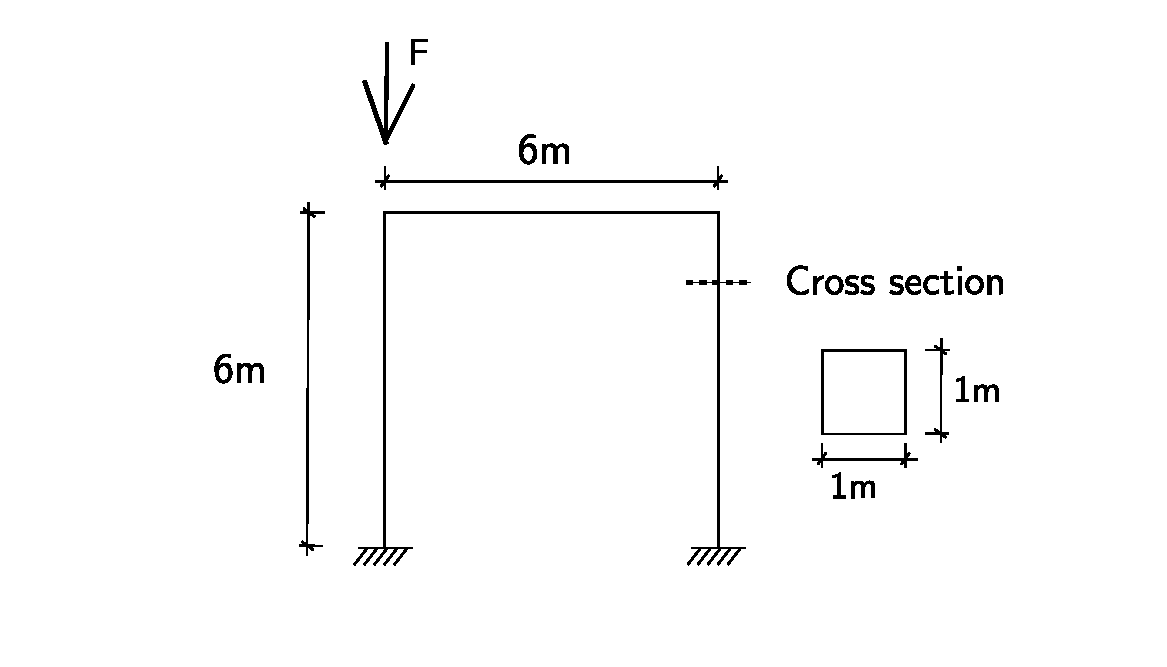
\includegraphics[width=10cm]{./Figure-files/_Chapter_Appendix_Illustrative_Examples/beam_elastic_frame_descrip.pdf}
  \caption{Elastic frame with \emph{beam\_elastic} elements.}
  \label{fig_frame}
\end{figure}





%%%%%%%%%%%%%%%%%%%%%%%%%%%%%%%%%%%%%%%%%%%%%%%%%%%%%%%%%%%%%%%%%%%%
\paragraph{ESSI model fei file:} ~

%\lstinputlisting[frame=single]{../Figure-files/1beam_elastic_presentation.fei}
\begin{lstlisting}
model name "beam_element_presentation" ;

add node # 1 at ( 0.00*m, 0.00*m, 0.00*m) with 6 dofs;
add node # 2 at ( 0.00*m, 0.00*m, 6.00*m) with 6 dofs;
add node # 3 at ( 6.00*m, 0.00*m, 6.00*m) with 6 dofs;
add node # 4 at ( 6.00*m, 0.00*m, 0.00*m) with 6 dofs;

elastic_constant  = 1e8*N/m^2; 
b=1*m;
h=1*m;
rho   = 0*kg/m^3;     // Mass density

add element # 1 type beam_elastic with nodes (1, 2) 
 cross_section =  b*h   elastic_modulus =  elastic_constant
 shear_modulus =  elastic_constant/2
 torsion_Jx =  0.33*b*h^3  bending_Iy =  b*h^3/12  bending_Iz =  h*b^3/12
 mass_density =   rho  xz_plane_vector = (1, 0, 1 ) 
   joint_1_offset = (0*m, 0*m, 0*m )  joint_2_offset = (0*m, 0*m, 0*m );

add element # 2 type beam_elastic with nodes (2,3) 
 cross_section =  b*h  elastic_modulus =  elastic_constant
 shear_modulus =  elastic_constant/2
 torsion_Jx =  0.33*b*h^3  bending_Iy =  b*h^3/12  bending_Iz =  h*b^3/12
 mass_density =   rho  xz_plane_vector = (1, 0, 1 ) 
   joint_1_offset = (0*m, 0*m, 0*m ) joint_2_offset = (0*m, 0*m, 0*m );

add element # 3 type beam_elastic with nodes (3,4) 
 cross_section =  b*h  elastic_modulus =  elastic_constant
 shear_modulus =  elastic_constant/2
 torsion_Jx =  0.33*b*h^3 bending_Iy =  b*h^3/12  bending_Iz =  h*b^3/12
 mass_density =   rho  xz_plane_vector = (1, 0, 1 ) 
   joint_1_offset = (0*m, 0*m, 0*m ) joint_2_offset = (0*m, 0*m, 0*m );

fix node #1 dofs all;
fix node #4 dofs all;

new loading stage "Fz";

add load # 1 to node # 2 type linear Fz=50*N;

define algorithm With_no_convergence_check;
define solver ProfileSPD;
define load factor increment 1;
simulate 1 steps using static algorithm;

bye;
\end{lstlisting}

The    ESSI   model   fei   files   for   this   example   can   be   downloaded
\href{https://github.com/BorisJeremic/Real-ESSI-Examples/blob/master/model_fei_file/beam_elastic_presentation_example/beam_elastic_presentation_example.tgz?raw=true}{here}.











%%%%%%%%%%%%%%%%%%%%%%%%%%%%%%%%%%%%%%%%%%%%%%%%%%%%%%%%%%%%%%%%%%%%%%%%%%%%%%%%
%%%%%%%%%%%%%%%%%%%%%%%%%%%%%%%%%%%%%%%%%%%%%%%%%%%%%%%%%%%%%%%%%%%%%%%%%%%%%%%%
%%%%%%%%%%%%%%%%%%%%%%%%%%%%%%%%%%%%%%%%%%%%%%%%%%%%%%%%%%%%%%%%%%%%%%%%%%%%%%%%
%%%%%%%%%%%%%%%%%%%%%%%%%%%%%%%%%%%%%%%%%%%%%%%%%%%%%%%%%%%%%%%%%%%%%%%%%%%%%%%%
%%%%%%%%%%%%%%%%%%%%%%%%%%%%%%%%%%%%%%%%%%%%%%%%%%%%%%%%%%%%%%%%%%%%%%%%%%%%%%%%
%%%%%%%%%%%%%%%%%%%%%%%%%%%%%%%%%%%%%%%%%%%%%%%%%%%%%%%%%%%%%%%%%%%%
\section{27NodeBrick Cantilever Beam for the static load}

%%%%%%%%%%%%%%%%%%%%%%%%%%%%%%%%%%%%%%%%%%%%%%%%%%%%%%%%%%%%%%%%%%%%
\paragraph{Problem description: } ~

Length=6m, Width=1m, Height=1m, Force=100N, E=1E8Pa, $\nu=0.0$.
The force direction is shown in Figure (\ref{fig Problem description for cantilever beams of different Poisson's 27}). 

\begin{figure}[!htb]
  \centering
  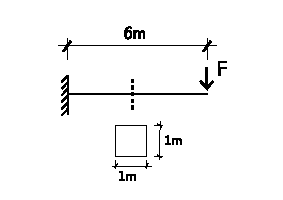
\includegraphics[width=7cm]{./Figure-files/_Chapter_Appendix_Illustrative_Examples/cantilever_6.pdf}
  \caption{Problem description for cantilever beam.}
  \label{fig Problem description for cantilever beams of different Poisson's 27}
\end{figure}

%%%%%%%%%%%%%%%%%%%%%%%%%%%%%%%%%%%%%%%%%%%%%%%%%%%%%%%%%%%%%%%%%%%%
\paragraph{Numerical model:} ~

The  27NodeBrick  elements  for  cantilever  beams  is shown in Figure (\ref{fig 27NodeBrick elements for cantilever beams of different Poisson's ratios}):

\begin{figure}[!htb]
  \centering
  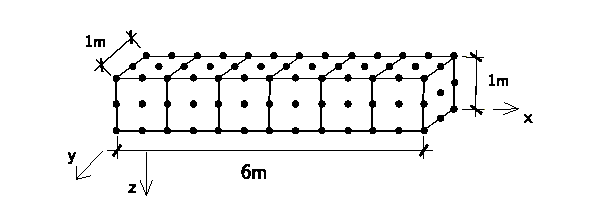
\includegraphics[width=9cm]{./Figure-files/_Chapter_Appendix_Illustrative_Examples/beam_27brick_6div.pdf}
  \caption{27NodeBrick elements for cantilever beams made of solid elements.}
  \label{fig 27NodeBrick elements for cantilever beams of different Poisson's ratios}
\end{figure}

%%%%%%%%%%%%%%%%%%%%%%%%%%%%%%%%%%%%%%%%%%%%%%%%%%%%%%%%%%%%%%%%%%%%
\paragraph{ESSI model fei file: } ~


%\lstinputlisting[frame=single]{../Figure-files/5_27NodeBrick.fei}
\begin{lstlisting}
model name "6meter_cantilever_27brick" ;

add material # 1 type linear_elastic_isotropic_3d
  mass_density = 0*kg/m^3
  elastic_modulus = 1e8*N/m^2
  poisson_ratio = 0.0;

add node #  1 at (   0.00 *m,   1.00 *m,  0.00 *m) with 3 dofs;
add node #  2 at (   0.00 *m,   0.00 *m,  0.00 *m) with 3 dofs;
add node #  3 at (   6.00 *m,   1.00 *m,  0.00 *m) with 3 dofs;
add node #  4 at (   5.00 *m,   1.00 *m,  0.00 *m) with 3 dofs;
add node #  5 at (   4.00 *m,   1.00 *m,  0.00 *m) with 3 dofs;
add node #  6 at (   3.00 *m,   1.00 *m,  0.00 *m) with 3 dofs;
...
...
add node #117 at (   5.50 *m,   0.50 *m,  1.00 *m) with 3 dofs;

add element #  1 type 27NodeBrickLT with nodes(   2,  10,  8,  1,  15,  17,  28,  23,  29,  30,  31,  32,  33,  34,  35,  36,  37,  38,  39,  40,  41,  42,  43,  44,  45,  46,  47) use material #  1; 
add element #  2 type 27NodeBrickLT with nodes(  10,  11,  7,  8,  17,  18,  27,  28,  48,  49,  50,  30,  51,  52,  53,  34,  38,  54,  55,  39,  56,  57,  58,  59,  43,  60,  61) use material #  1; 
add element #  3 type 27NodeBrickLT with nodes(  11,  12,  6,  7,  18,  19,  26,  27,  62,  63,  64,  49,  65,  66,  67,  52,  54,  68,  69,  55,  70,  71,  72,  73,  58,  74,  75) use material #  1; 
add element #  4 type 27NodeBrickLT with nodes(  12,  13,  5,  6,  19,  20,  25,  26,  76,  77,  78,  63,  79,  80,  81,  66,  68,  82,  83,  69,  84,  85,  86,  87,  72,  88,  89) use material #  1; 
add element #  5 type 27NodeBrickLT with nodes(  13,  14,  4,  5,  20,  21,  24,  25,  90,  91,  92,  77,  93,  94,  95,  80,  82,  96,  97,  83,  98,  99, 100, 101,  86, 102, 103) use material #  1; 
add element #  6 type 27NodeBrickLT with nodes(  14,  9,   3,  4,  21,  16,  22,  24, 104, 105, 106,  91, 107, 108, 109,  94,  96, 110, 111,  97, 112, 113, 114, 115, 100, 116, 117) use material #  1; 

fix node # 1 dofs all;
fix node # 2 dofs all;
fix node # 15 dofs all;
fix node # 23 dofs all;
fix node # 32 dofs all;
fix node # 36 dofs all;
fix node # 37 dofs all;
fix node # 40 dofs all;
fix node # 45 dofs all;

new loading stage "Fz";
add load # 1 to node # 13 type linear Fz=2.777778*N; 
add load # 2 to node # 24 type linear Fz=2.777778*N; 
add load # 3 to node # 3 type linear Fz=2.777778*N; 
add load # 4 to node # 34 type linear Fz=2.777778*N; 
add load # 5 to node # 182 type linear Fz=11.111111*N; 
add load # 6 to node # 177 type linear Fz=11.111111*N; 
add load # 7 to node # 180 type linear Fz=11.111111*N; 
add load # 8 to node # 183 type linear Fz=11.111111*N; 
add load # 9 to node # 186 type linear Fz=44.444444*N; 

define algorithm With_no_convergence_check ;
define solver UMFPack;
define load factor increment 1;
simulate 1 steps using static algorithm;

bye;
\end{lstlisting}

The ESSI model fei files for this example can be downloaded 
\href{https://github.com/BorisJeremic/Real-ESSI-Examples/blob/master/model_fei_file/27NodeBrick_static/27NodeBrick_static.tgz?raw=true}{here}.









%%%%%%%%%%%%%%%%%%%%%%%%%%%%%%%%%%%%%%%%%%%%%%%%%%%%%%%%%%%%%%%%%%%%















%%%%%%%%%%%%%%%%%%%%%%%%%%%%%%%%%%%%%%%%%%%%%%%%%%%%%%%%%%%%%%%%%%%%%%%%%%%%%%%%
%%%%%%%%%%%%%%%%%%%%%%%%%%%%%%%%%%%%%%%%%%%%%%%%%%%%%%%%%%%%%%%%%%%%%%%%%%%%%%%%
%%%%%%%%%%%%%%%%%%%%%%%%%%%%%%%%%%%%%%%%%%%%%%%%%%%%%%%%%%%%%%%%%%%%%%%%%%%%%%%%
%%%%%%%%%%%%%%%%%%%%%%%%%%%%%%%%%%%%%%%%%%%%%%%%%%%%%%%%%%%%%%%%%%%%%%%%%%%%%%%%
%%%%%%%%%%%%%%%%%%%%%%%%%%%%%%%%%%%%%%%%%%%%%%%%%%%%%%%%%%%%%%%%%%%%%%%%%%%%%%%%
%%%%%%%%%%%%%%%%%%%%%%%%%%%%%%%%%%%%%%%%%%%%%%%%%%%%%%%%%%%%%%%%%%%%
%%%%%%%%%%%%%%%%%%%%%%%%%%%%%%%%%%%%%%%%%%%%%%%%%%%%%%%%%%%%%%%%%%%%
\section{4NodeANDES Cantilever Beams Under the Force Perpendicular to Plane}

%%%%%%%%%%%%%%%%%%%%%%%%%%%%%%%%%%%%%%%%%%%%%%%%%%%%%%%%%%%%%%%%%%%%
\paragraph{Problem description:} ~

Length=6m, Width=1m, Height=1m, Force=100N, E=1E8Pa, $\nu=0.0$. 

\begin{figure}[!htb]
  \centering
  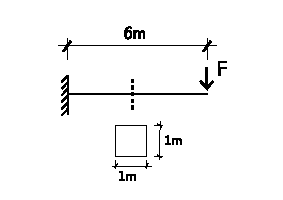
\includegraphics[width=7cm]{./Figure-files/_Chapter_Appendix_Illustrative_Examples/cantilever_6.pdf}
  \caption{Cantilever beams}
  \label{fig Problem description for cantilever 4}
\end{figure}


%%%%%%%%%%%%%%%%%%%%%%%%%%%%%%%%%%%%%%%%%%%%%%%%%%%%%%%%%%%%%%%%%%%%
\paragraph{Numerical model:} ~

\vskip 12pt

For a force  direction  perpendicular  to  the  plane, only the bending
deformation is present.


The  model is shown  in Figure (\ref{fig 4NodeANDES elements for
cantilever beams under force perpendicular to plane}).

\begin{figure}[!htb]
  \centering
%  \begin{subfigure}{0.5\textwidth}
    \centering
    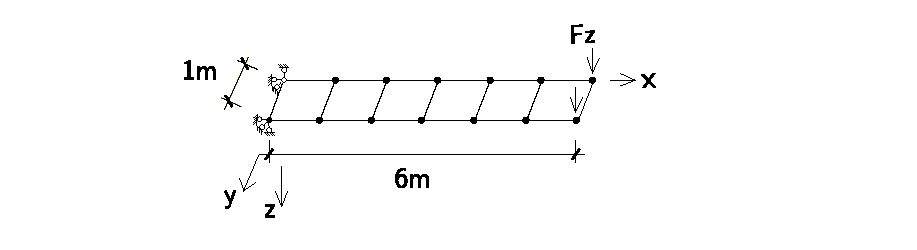
\includegraphics[width=10cm]{./Figure-files/_Chapter_Appendix_Illustrative_Examples/beam_ANDES_xy_bending_6div.pdf}
%    % \caption{Six 4NodeANDES elements}
%  \end{subfigure}
%  \captionsetup{justification=centering,margin=3cm}
  \caption{4NodeANDES elements for cantilever beams under force perpendicular to
  plane.}
  \label{fig 4NodeANDES elements for cantilever beams under force perpendicular to plane}
\end{figure}


%%%%%%%%%%%%%%%%%%%%%%%%%%%%%%%%%%%%%%%%%%%%%%%%%%%%%%%%%%%%%%%%%%%%
\paragraph{ESSI model fei file: } ~

%\lstinputlisting[frame=single]{../Figure-files/3_perpend_ANDES.fei}
\begin{lstlisting}
 model name "6meter_cantilever_4NodeANDES" ;
      
add material # 1 type linear_elastic_isotropic_3d
  mass_density = 0*kg/m^3
  elastic_modulus = 1e8*N/m^2
  poisson_ratio = 0.0;

add node #  1 at ( 0.0*m, 0.0*m, 0.0*m) with 6 dofs;
add node #  2 at ( 6.0*m, 0.0*m, 0.0*m) with 6 dofs;
add node #  3 at ( 1.0*m, 0.0*m, 0.0*m) with 6 dofs;
add node #  4 at ( 2.0*m, 0.0*m, 0.0*m) with 6 dofs;
add node #  5 at ( 3.0*m, 0.0*m, 0.0*m) with 6 dofs;
add node #  6 at ( 4.0*m, 0.0*m, 0.0*m) with 6 dofs;
add node #  7 at ( 5.0*m, 0.0*m, 0.0*m) with 6 dofs;
add node #  8 at ( 6.0*m, 1.0*m, 0.0*m) with 6 dofs;
add node #  9 at ( 0.0*m, 1.0*m, 0.0*m) with 6 dofs;
add node # 10 at ( 5.0*m, 1.0*m, 0.0*m) with 6 dofs;
add node # 11 at ( 4.0*m, 1.0*m, 0.0*m) with 6 dofs;
add node # 12 at ( 3.0*m, 1.0*m, 0.0*m) with 6 dofs;
add node # 13 at ( 2.0*m, 1.0*m, 0.0*m) with 6 dofs;
add node # 14 at ( 1.0*m, 1.0*m, 0.0*m) with 6 dofs;

h = 1*m; 
add element # 1 type 4NodeShell_ANDES with nodes (1,3,14,9) use material # 1 thickness = h ; 
add element # 2 type 4NodeShell_ANDES with nodes (3,4,13,14) use material # 1 thickness = h ; 
add element # 3 type 4NodeShell_ANDES with nodes (4,5,12,13) use material # 1 thickness = h ; 
add element # 4 type 4NodeShell_ANDES with nodes (5,6,11,12) use material # 1 thickness = h ; 
add element # 5 type 4NodeShell_ANDES with nodes (6,7,10,11) use material # 1 thickness = h ; 
add element # 6 type 4NodeShell_ANDES with nodes (7,2,8,10) use material # 1 thickness = h ; 

fix node #  1 dofs all    ;
fix node #  9 dofs all    ;

new loading stage "Fz";
add load # 1 to node # 8 type linear Fz=50*N;
add load # 2 to node # 2 type linear Fz=50*N;

define algorithm With_no_convergence_check ;
define solver ProfileSPD;
define load factor increment 1;
simulate 1 steps using static algorithm;

bye;
\end{lstlisting}

The ESSI model fei files for this example can be downloaded 
\href{https://github.com/BorisJeremic/Real-ESSI-Examples/blob/master/model_fei_file/ANDESshell_cantilever_perpendicular_to_plane/ANDESshell_cantilever_perpendicular_to_plane.tgz?raw=true}{here}.








%%%%%%%%%%%%%%%%%%%%%%%%%%%%%%%%%%%%%%%%%%%%%%%%%%%%%%%%%%%%%%%%%%%%













%%%%%%%%%%%%%%%%%%%%%%%%%%%%%%%%%%%%%%%%%%%%%%%%%%%%%%%%%%%%%%%%%%%%%%%%%%%%%%%%
%%%%%%%%%%%%%%%%%%%%%%%%%%%%%%%%%%%%%%%%%%%%%%%%%%%%%%%%%%%%%%%%%%%%%%%%%%%%%%%%
%%%%%%%%%%%%%%%%%%%%%%%%%%%%%%%%%%%%%%%%%%%%%%%%%%%%%%%%%%%%%%%%%%%%%%%%%%%%%%%%
%%%%%%%%%%%%%%%%%%%%%%%%%%%%%%%%%%%%%%%%%%%%%%%%%%%%%%%%%%%%%%%%%%%%%%%%%%%%%%%%
%%%%%%%%%%%%%%%%%%%%%%%%%%%%%%%%%%%%%%%%%%%%%%%%%%%%%%%%%%%%%%%%%%%%%%%%%%%%%%%%
%%%%%%%%%%%%%%%%%%%%%%%%%%%%%%%%%%%%%%%%%%%%%%%%%%%%%%%%%%%%%%%%%%%
\section{4NodeANDES Cantilever Beams under the In-Plane Force}

%%%%%%%%%%%%%%%%%%%%%%%%%%%%%%%%%%%%%%%%%%%%%%%%%%%%%%%%%%%%%%%%%%%%
\paragraph{Problem description:} ~

Length=6m, Width=1m, Height=1m, Force=100N, E=1E8Pa, $\nu=0.0$. 

\begin{figure}[!htb]
  \centering
  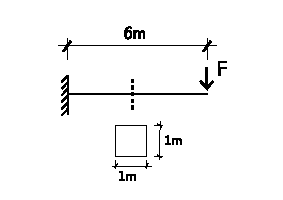
\includegraphics[width=7cm]{./Figure-files/_Chapter_Appendix_Illustrative_Examples/cantilever_6.pdf}
  \caption{Problem description for cantilever beams with in plane force}
  \label{fig Problem description for cantilever 4 2}
\end{figure}

%%%%%%%%%%%%%%%%%%%%%%%%%%%%%%%%%%%%%%%%%%%%%%%%%%%%%%%%%%%%%%%%%%%%
\paragraph{Numerical model:} ~

%When the force direction is inplane, both the bending and shear deformation are calculated in 4NodeANDES elements. 
\begin{lstlisting}

\end{lstlisting}

The 4NodeANDES elements under in-plane force is shown in Figure (\ref{fig 4NodeANDES elements for cantilever beams under inplane force}).

\begin{figure}[!htb]
  \centering
  \vskip 8pt
%  \begin{subfigure}{0.5\textwidth}
    \centering
    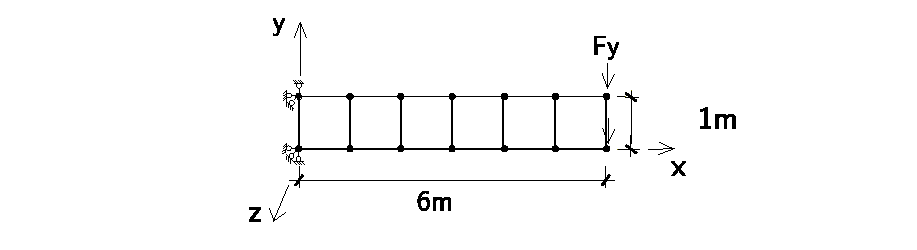
\includegraphics[width=10cm]{./Figure-files/_Chapter_Appendix_Illustrative_Examples/beam_ANDES_yz_inPlane_6div.pdf}
%  \end{subfigure}
%  \captionsetup{justification=centering,margin=3cm}
  \caption{4NodeANDES elements for cantilever beams under in-plane force}
  \label{fig 4NodeANDES elements for cantilever beams under inplane force}
\end{figure}


%%%%%%%%%%%%%%%%%%%%%%%%%%%%%%%%%%%%%%%%%%%%%%%%%%%%%%%%%%%%%%%%%%%%
\paragraph{ESSI model fei file: } ~

%\lstinputlisting[frame=single]{../Figure-files/4_inplane_ANDES.fei}
\begin{lstlisting}
model name "6meter_cantilever_4NodeANDES" ;

add material # 1 type linear_elastic_isotropic_3d
  mass_density = 0*kg/m^3
  elastic_modulus = 1e8*N/m^2
  poisson_ratio = 0.0;

add node #   1 at ( 0.00*m, 0.00*m, 0.00*m) with 6 dofs;
add node #   2 at ( 6.00*m, 0.00*m, 0.00*m) with 6 dofs;
add node #   3 at ( 1.00*m, 0.00*m, 0.00*m) with 6 dofs;
add node #   4 at ( 2.00*m, 0.00*m, 0.00*m) with 6 dofs;
add node #   5 at ( 3.00*m, 0.00*m, 0.00*m) with 6 dofs;
add node #   6 at ( 4.00*m, 0.00*m, 0.00*m) with 6 dofs;
add node #   7 at ( 5.00*m, 0.00*m, 0.00*m) with 6 dofs;
add node #   8 at ( 6.00*m, 1.00*m, 0.00*m) with 6 dofs;
add node #   9 at ( 0.00*m, 1.00*m, 0.00*m) with 6 dofs;
add node #  10 at ( 5.00*m, 1.00*m, 0.00*m) with 6 dofs;
add node #  11 at ( 4.00*m, 1.00*m, 0.00*m) with 6 dofs;
add node #  12 at ( 3.00*m, 1.00*m, 0.00*m) with 6 dofs;
add node #  13 at ( 2.00*m, 1.00*m, 0.00*m) with 6 dofs;
add node #  14 at ( 1.00*m, 1.00*m, 0.00*m) with 6 dofs;

h     = 1*m;  
add element # 1 type 4NodeShell_ANDES with nodes (1,3,14,9) use material # 1 thickness = h ; 
add element # 2 type 4NodeShell_ANDES with nodes (3,4,13,14) use material # 1 thickness = h ; 
add element # 3 type 4NodeShell_ANDES with nodes (4,5,12,13) use material # 1 thickness = h ; 
add element # 4 type 4NodeShell_ANDES with nodes (5,6,11,12) use material # 1 thickness = h ; 
add element # 5 type 4NodeShell_ANDES with nodes (6,7,10,11) use material # 1 thickness = h ; 
add element # 6 type 4NodeShell_ANDES with nodes (7,2,8,10) use material # 1 thickness = h ; 

fix node #  1 dofs all;
fix node #  9 dofs all;

new loading stage "Fy";
add load # 1 to node # 8 type linear Fy=50*N;
add load # 2 to node # 2 type linear Fy=50*N;

define algorithm With_no_convergence_check ;
define solver ProfileSPD;
define load factor increment 1;
simulate 1 steps using static algorithm;

bye;
\end{lstlisting}


The ESSI model fei files for this example can be downloaded 
\href{https://github.com/BorisJeremic/Real-ESSI-Examples/blob/master/model_fei_file/ANDESshell_cantilever_inplane/ANDESshell_cantilever_inplane.tgz?raw=true}{here}.








%%%%%%%%%%%%%%%%%%%%%%%%%%%%%%%%%%%%%%%%%%%%%%%%%%%%%%%%%%%%%%%%%%%%
























%%%%%%%%%%%%%%%%%%%%%%%%%%%%%%%%%%%%%%%%%%%%%%%%%%%%%%%%%%%%%%%%%%%%%%%%%%%%%%%%
%%%%%%%%%%%%%%%%%%%%%%%%%%%%%%%%%%%%%%%%%%%%%%%%%%%%%%%%%%%%%%%%%%%%%%%%%%%%%%%%
%%%%%%%%%%%%%%%%%%%%%%%%%%%%%%%%%%%%%%%%%%%%%%%%%%%%%%%%%%%%%%%%%%%%%%%%%%%%%%%%
%%%%%%%%%%%%%%%%%%%%%%%%%%%%%%%%%%%%%%%%%%%%%%%%%%%%%%%%%%%%%%%%%%%%%%%%%%%%%%%%
%%%%%%%%%%%%%%%%%%%%%%%%%%%%%%%%%%%%%%%%%%%%%%%%%%%%%%%%%%%%%%%%%%%%%%%%%%%%%%%%
%%%%%%%%%%%%%%%%%%%%%%%%%%%%%%%%%%%%%%%%%%%%%%%%%%%%%%%%%%%%%%%%%%%%
\section{27NodeBrick Cantilever Beams for Dynamic Loading}



%%%%%%%%%%%%%%%%%%%%%%%%%%%%%%%%%%%%%%%%%%%%%%%%%%%%%%%%%%%%%%%%%%%%
\paragraph{Problem description:} ~



Length=20m, Width=1m, Height=1m, E=504MPa, $\nu=0.4$. 

All degree of freedoms at the bottom nodes are fixed. 

The load is a self weight with a dynamic displacement of supports.


\begin{figure}[!htb]
  \centering
  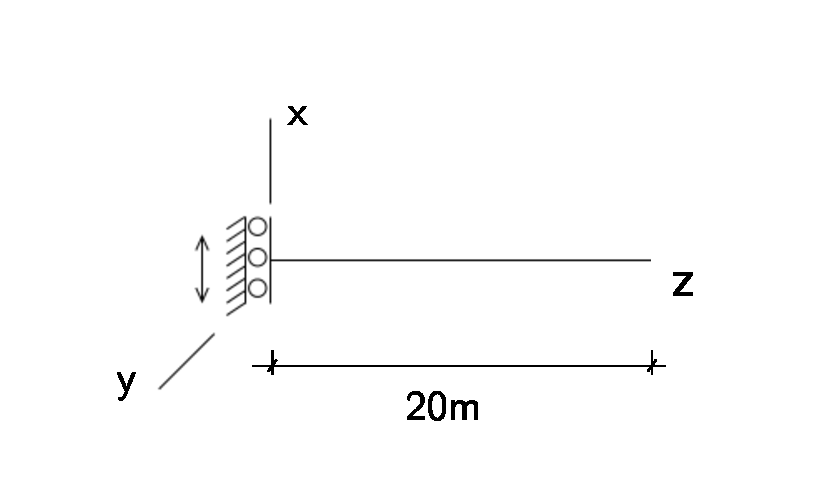
\includegraphics[width=8cm]{./Figure-files/_Chapter_Appendix_Illustrative_Examples/dynamic_example_diagram.pdf}
  \caption{Problem description for one simple dynamic example}
  \label{fig Problem description for one simple dynamic example}
\end{figure}



%%%%%%%%%%%%%%%%%%%%%%%%%%%%%%%%%%%%%%%%%%%%%%%%%%%%%%%%%%%%%%%%%%%%
\paragraph{Numerical model:} ~

The numerical model applied 27NodeBrick to simulate the 1D motion. 

\begin{figure}[!htb]
  \centering
  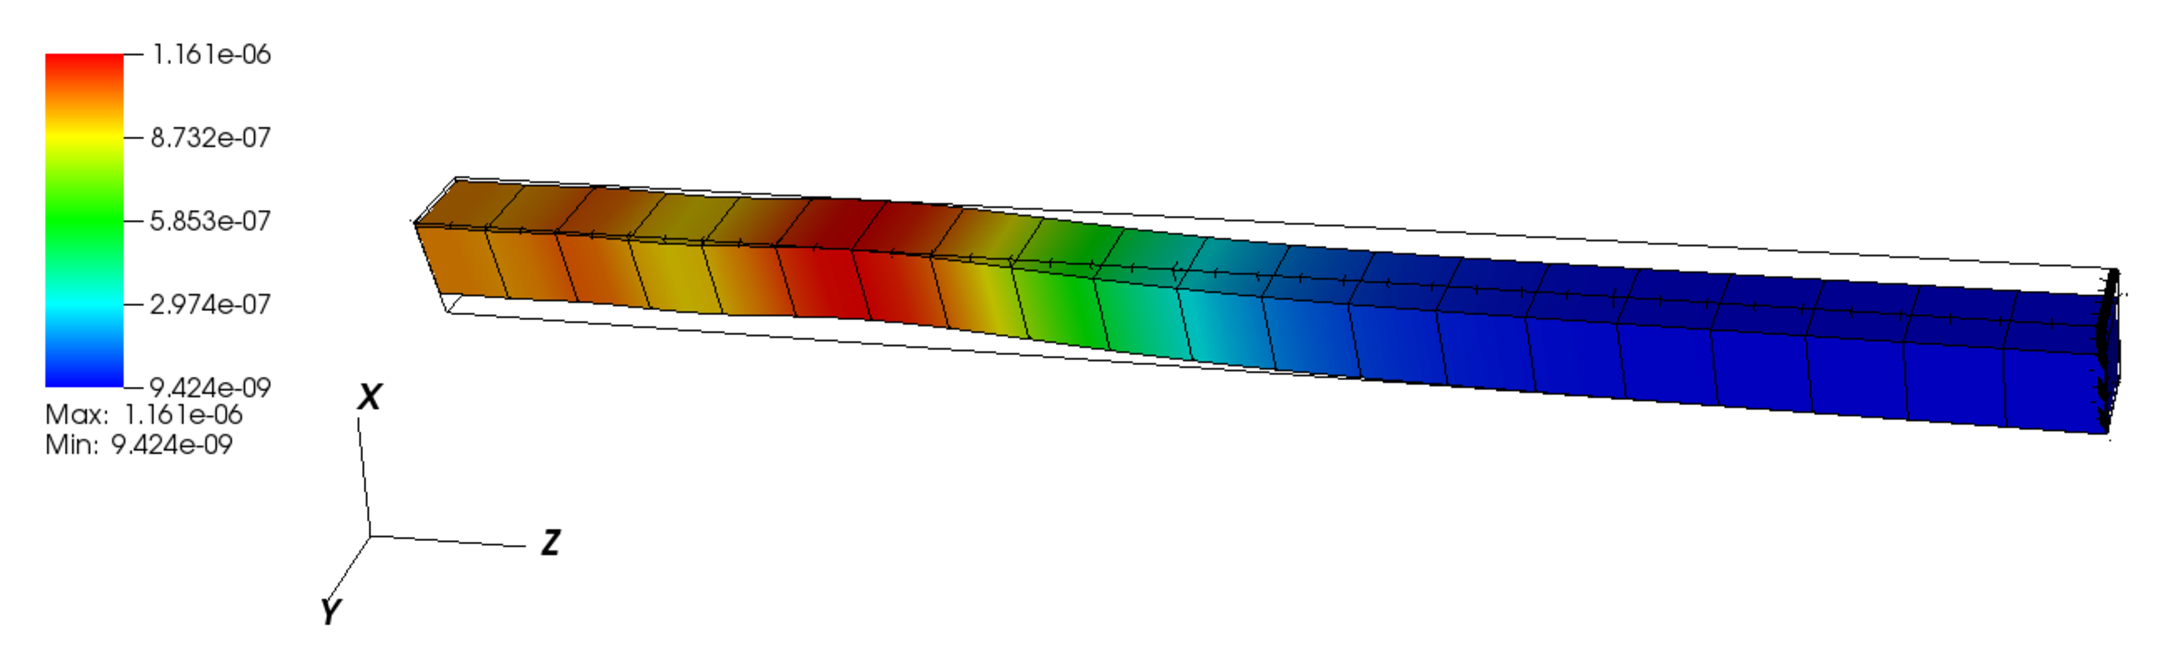
\includegraphics[width=16cm]{./Figure-files/_Chapter_Appendix_Illustrative_Examples/dynamic_example_numerical.pdf}
  \caption{Numerical model for one simple dynamic example}
  \label{fig Numerical model for one simple dynamic example}
\end{figure}

%%%%%%%%%%%%%%%%%%%%%%%%%%%%%%%%%%%%%%%%%%%%%%%%%%%%%%%%%%%%%%%%%%%%
\paragraph{ESSI model fei file: } ~

%\lstinputlisting[frame=single]{../Figure-files/6dynamic_example.fei}
\begin{lstlisting}
model name "dynamic_example";

add material # 1 type linear_elastic_isotropic_3d_LT
 mass_density    = 2000*kg/m^3
 elastic_modulus = 504000000.00*Pa
 poisson_ratio   = 0.4;

add node No 1 at (0*m, 0*m, 0*m) with 3 dofs;
add node No 2 at (0*m, 0.5*m, 0*m) with 3 dofs;
add node No 3 at (0*m, 1*m, 0*m) with 3 dofs;
add node No 4 at (0.5*m, 0*m, 0*m) with 3 dofs;
add node No 5 at (0.5*m, 0.5*m, 0*m) with 3 dofs;
add node No 6 at (0.5*m, 1*m, 0*m) with 3 dofs;
...
...
add node No 369 at (1*m, 1*m, 20*m) with 3 dofs;

add element # 1 type 27NodeBrickLT with nodes (27,21,19,25,9,3,1,7,24,20,22,26,6,2,4,8,18,12,10,16,14,15,11,13,17,23,5) use material # 1 ;
add element # 2 type 27NodeBrickLT with nodes (45,39,37,43,27,21,19,25,42,38,40,44,24,20,22,26,36,30,28,34,32,33,29,31,35,41,23) use material # 1 ;
add element # 3 type 27NodeBrickLT with nodes (63,57,55,61,45,39,37,43,60,56,58,62,42,38,40,44,54,48,46,52,50,51,47,49,53,59,41) use material # 1 ;
add element # 4 type 27NodeBrickLT with nodes (81,75,73,79,63,57,55,61,78,74,76,80,60,56,58,62,72,66,64,70,68,69,65,67,71,77,59) use material # 1 ;
add element # 5 type 27NodeBrickLT with nodes (99,93,91,97,81,75,73,79,96,92,94,98,78,74,76,80,90,84,82,88,86,87,83,85,89,95,77) use material # 1 ;
...
...
add element # 20 type 27NodeBrickLT with nodes (369,363,361,367,351,345,343,349,366,362,364,368,348,
 344,346,350,360,354,352,358,356,357,353,355,359,365,347) use material # 1 ;

add acceleration field # 1 ax = 0*g ay = 0*g az = -1*g ;
add load # 1 to element # 1 type self_weight use acceleration field # 1;
add load # 2 to element # 2 type self_weight use acceleration field # 1;
add load # 3 to element # 3 type self_weight use acceleration field # 1;
add load # 4 to element # 4 type self_weight use acceleration field # 1;
add load # 5 to element # 5 type self_weight use acceleration field # 1;
add load # 6 to element # 6 type self_weight use acceleration field # 1;
...
...
add load # 20 to element # 20 type self_weight use acceleration field # 1;

fix node No 1 dofs    uy uz;
fix node No 2 dofs    uy uz;
fix node No 3 dofs    uy uz;
fix node No 4 dofs    uy uz;
fix node No 5 dofs    uy uz;
fix node No 6 dofs    uy uz;
...
...
fix node No 369 dofs    uy uz;

zeta = 0.0166667;
fq1  = 3.75;
fq2  = 11.25;
omega1 = 2*pi*fq1;
omega2 = 2*pi*fq2;
zeta1 = zeta;
zeta2 = zeta;
alpha1 = 2*omega1*omega2*(zeta1*omega2-zeta2*omega1)/(omega2*omega2-omega1*omega1);
beta1  = 2*              (zeta2*omega2-zeta1*omega1)/(omega2*omega2-omega1*omega1);
add damping # 1 
   type Rayleigh 
   with 
   a0 = alpha1/s 
   a1 = beta1*s 
   stiffness_to_use = Initial_Stiffness;

add damping # 1 to element # 1;
add damping # 1 to element # 2;
add damping # 1 to element # 3;
add damping # 1 to element # 4;
add damping # 1 to element # 5;
add damping # 1 to element # 6;
...
...
add damping # 1 to element # 20;

new loading stage "impose_motion";

add imposed motion # 1001 to node # 1 dof ux 
 displacement_scale_unit = 1*m       displacement_file    = "dis.txt" 
 velocity_scale_unit     = 1*m/s     velocity_file        = "vel.txt" 
 acceleration_scale_unit = 1*m/s^2   acceleration_file    = "acc.txt";

add imposed motion # 1002 to node # 2 dof ux 
 displacement_scale_unit = 1*m         displacement_file    = "dis.txt" 
 velocity_scale_unit     = 1*m/s       velocity_file        = "vel.txt" 
 acceleration_scale_unit = 1*m/s^2     acceleration_file    = "acc.txt";

add imposed motion # 1003 to node # 3 dof ux 
 displacement_scale_unit = 1*m         displacement_file   = "dis.txt" 
 velocity_scale_unit     = 1*m/s       velocity_file       = "vel.txt" 
 acceleration_scale_unit = 1*m/s^2     acceleration_file   = "acc.txt";
...
...
add imposed motion # 1009 to node # 9 dof ux 
 displacement_scale_unit = 1*m        displacement_file   = "dis.txt" 
 velocity_scale_unit     = 1*m/s      velocity_file       = "vel.txt" 
 acceleration_scale_unit = 1*m/s^2    acceleration_file   = "acc.txt";

define dynamic integrator Newmark with gamma = 0.5 beta = 0.25;
define algorithm With_no_convergence_check;
define solver ProfileSPD;
simulate 50 steps using transient algorithm time_step = 0.005*s;
         
bye;
\end{lstlisting}


The ESSI model fei files for this example can be downloaded 
\href{https://github.com/BorisJeremic/Real-ESSI-Examples/blob/master/model_fei_file/27NodeBrick_dynamic_impose_motion/27NodeBrick_dynamic_impose_motion.tgz?raw=true}{here}.











%%%%%%%%%%%%%%%%%%%%%%%%%%%%%%%%%%%%%%%%%%%%%%%%%%%%%%%%%%%%%%%%%%%%













%%%%%%%%%%%%%%%%%%%%%%%%%%%%%%%%%%%%%%%%%%%%%%%%%%%%%%%%%%%%%%%%%%%%%%%%%%%%%%%%
%%%%%%%%%%%%%%%%%%%%%%%%%%%%%%%%%%%%%%%%%%%%%%%%%%%%%%%%%%%%%%%%%%%%%%%%%%%%%%%%
%%%%%%%%%%%%%%%%%%%%%%%%%%%%%%%%%%%%%%%%%%%%%%%%%%%%%%%%%%%%%%%%%%%%%%%%%%%%%%%%
%%%%%%%%%%%%%%%%%%%%%%%%%%%%%%%%%%%%%%%%%%%%%%%%%%%%%%%%%%%%%%%%%%%%%%%%%%%%%%%%
%%%%%%%%%%%%%%%%%%%%%%%%%%%%%%%%%%%%%%%%%%%%%%%%%%%%%%%%%%%%%%%%%%%%%%%%%%%%%%%%
%%%%%%%%%%%%%%%%%%%%%%%%%%%%%%%%%%%%%%%%%%%%%%%%%%%%%%%%%%%%%%%%%%%%
\section{4NodeANDES Square Plate with Four Edges Clamped}



%%%%%%%%%%%%%%%%%%%%%%%%%%%%%%%%%%%%%%%%%%%%%%%%%%%%%%%%%%%%%%%%%%%%
\paragraph{Problem description:} ~



Length=20m, Width=20m, Height=1m, Force=100N, E=1E8Pa, $\nu=0.3$. 

The four edges are \textbf{clamped}. 

The load is a self weight.


\begin{figure}[!htb]
  \centering
  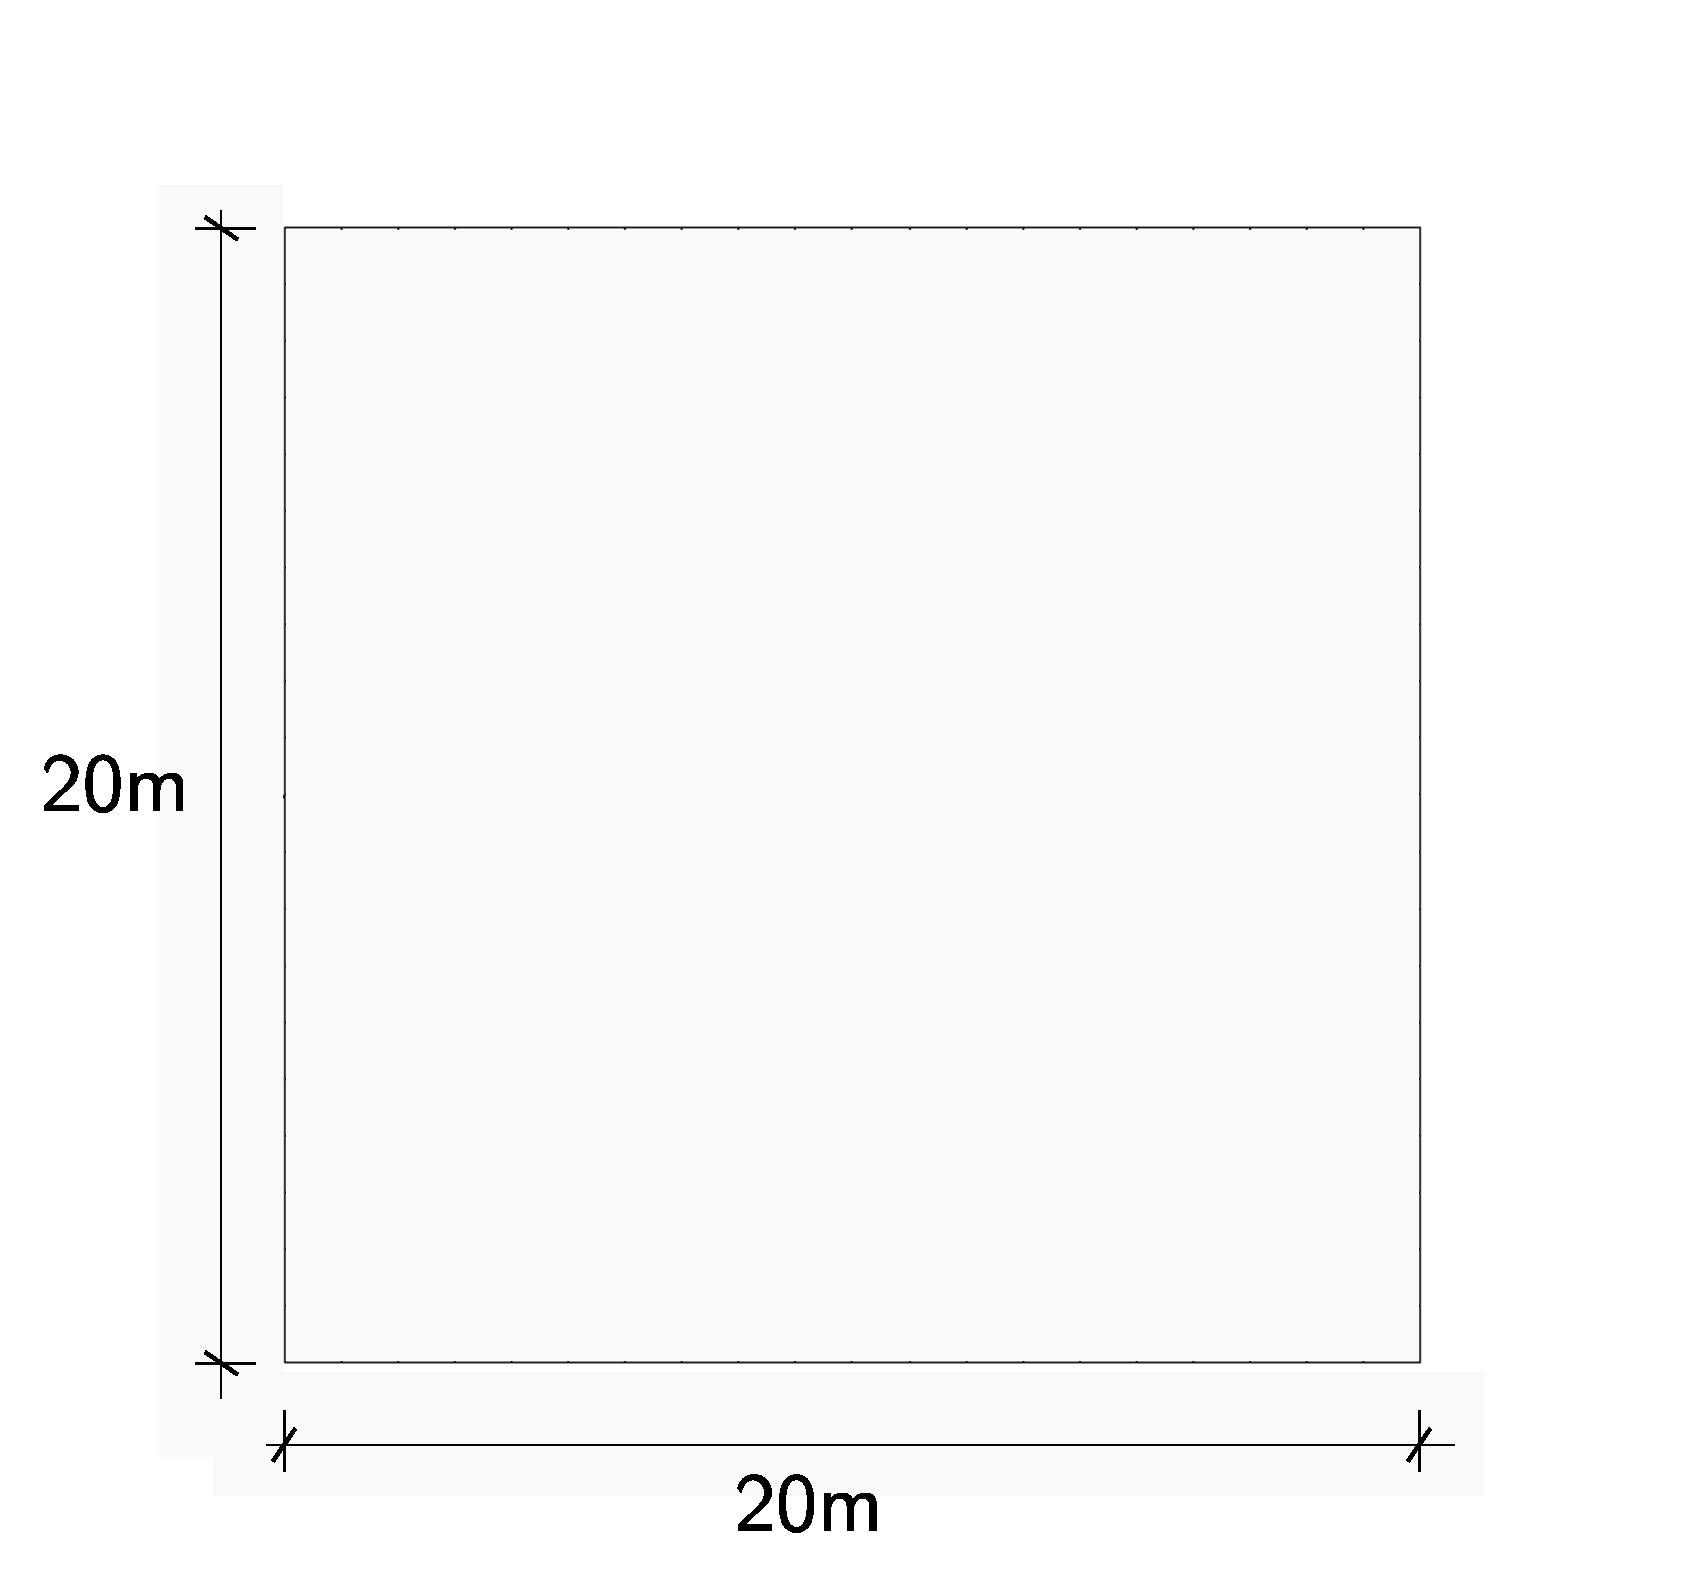
\includegraphics[width=10cm]{./Figure-files/_Chapter_Appendix_Illustrative_Examples/square_plate_descrp.pdf}
  \caption{Square plate with four edges clamped }
  \label{fig 4NodeANDES edges clamped square plate with element side length for program description }
\end{figure}


\clearpage
%%%%%%%%%%%%%%%%%%%%%%%%%%%%%%%%%%%%%%%%%%%%%%%%%%%%%%%%%%%%%%%%%%%%
\paragraph{Numerical model:} ~

The element side length is 1 meter. 


\begin{figure}[!htb]
  \centering
  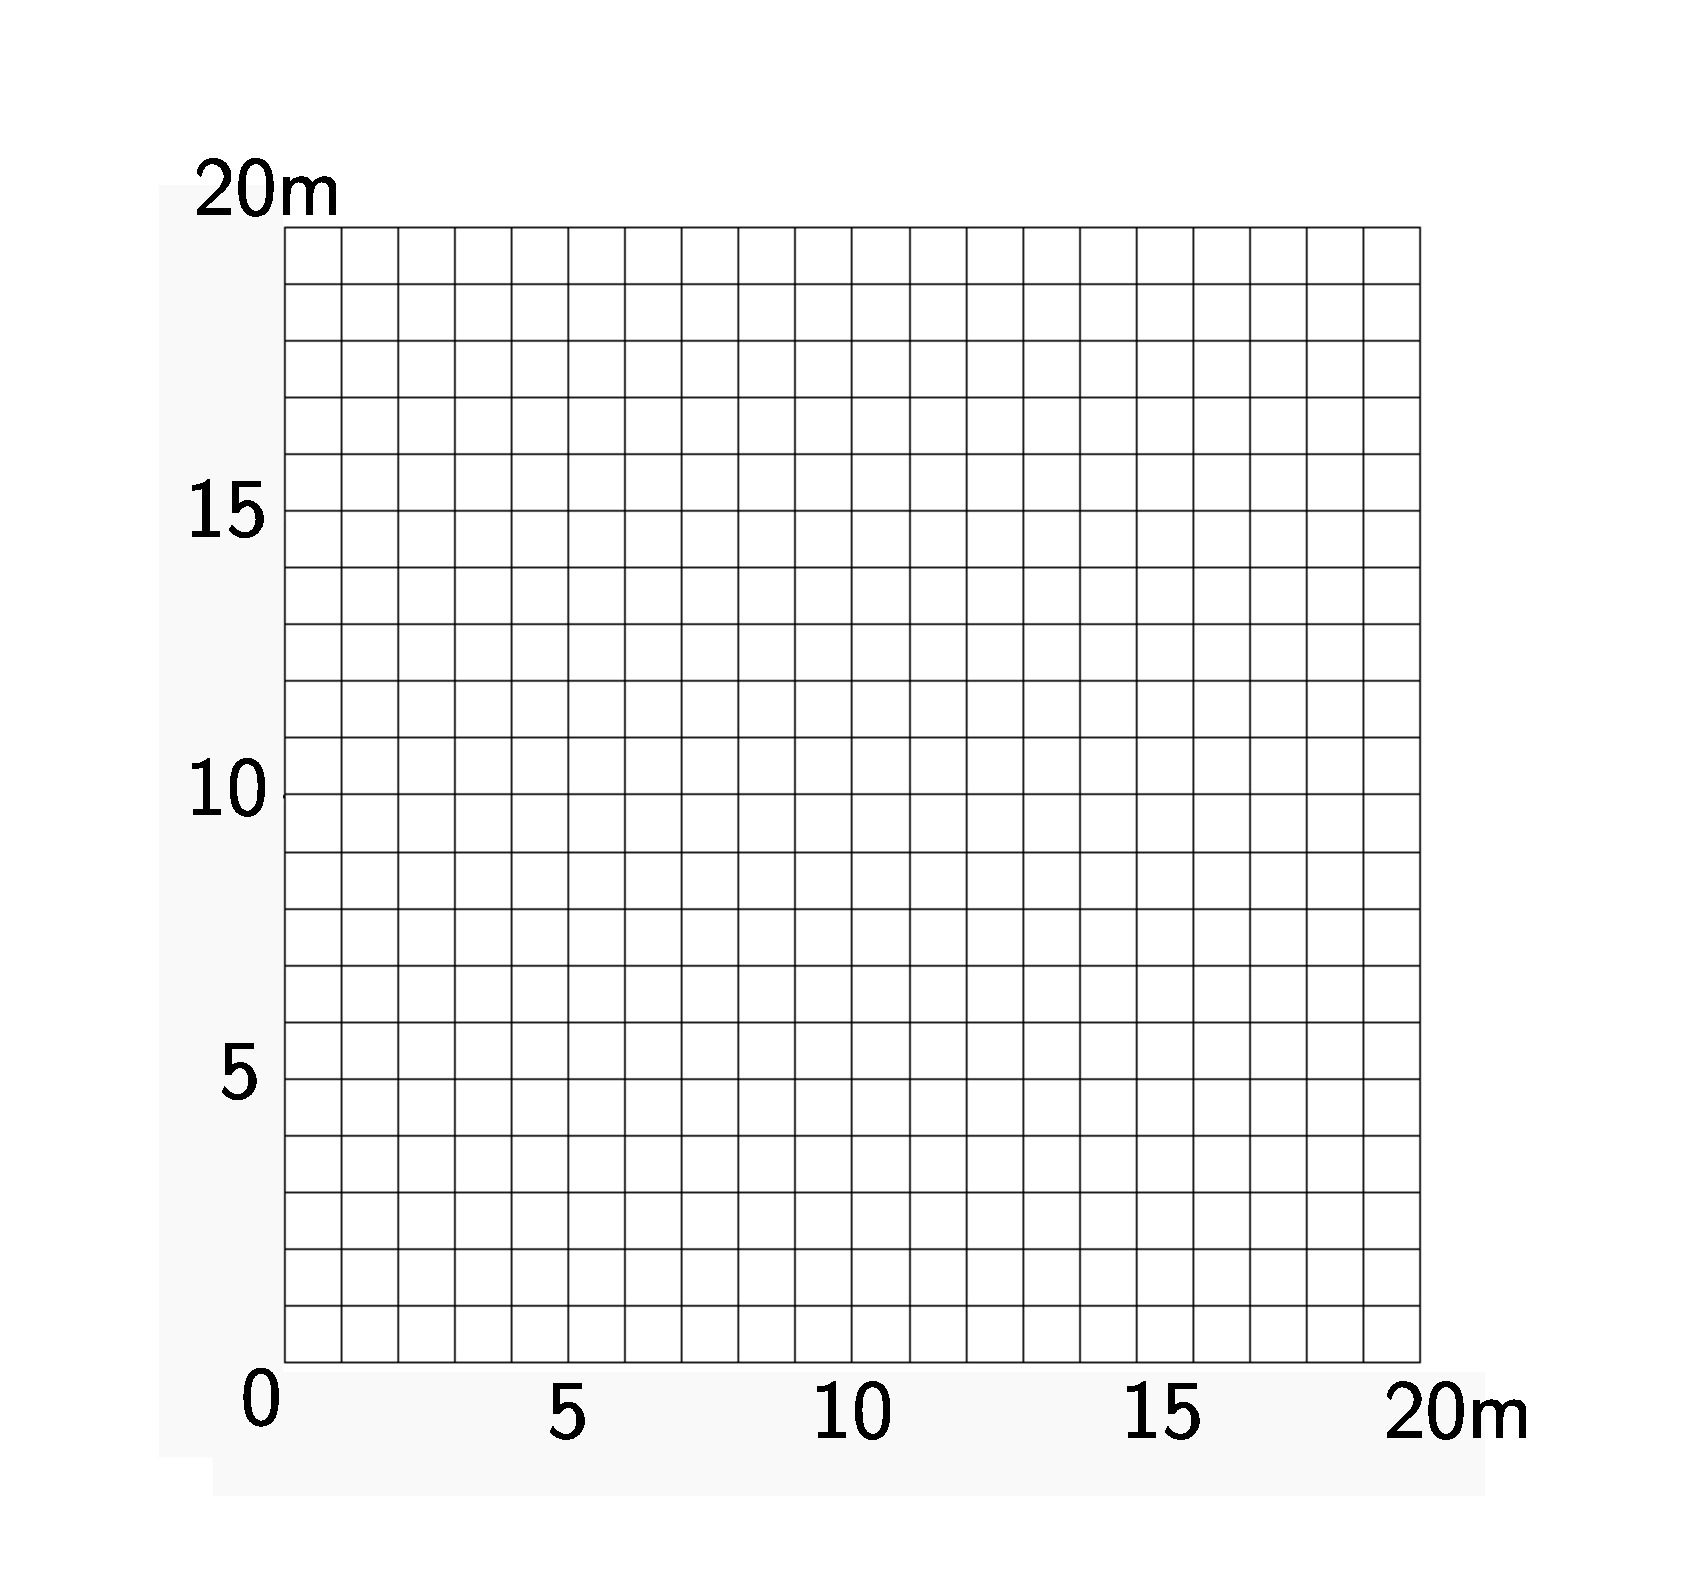
\includegraphics[width=10cm]{./Figure-files/_Chapter_Appendix_Illustrative_Examples/square_plate4_2.pdf}
  \caption{4NodeANDES edge clamped square plate with element side length 1m }
  \label{fig 4NodeANDES edges clamped square plate with element side length 1m }
\end{figure}


%%%%%%%%%%%%%%%%%%%%%%%%%%%%%%%%%%%%%%%%%%%%%%%%%%%%%%%%%%%%%%%%%%%%
\paragraph{ESSI model fei file: } ~


%\lstinputlisting[frame=single]{../Figure-files/7shell.fei}
\begin{lstlisting}
model name "square_plate" ;

add material # 1 type linear_elastic_isotropic_3d
  mass_density = 1e2*kg/m^3   elastic_modulus = 1e8*N/m^2   poisson_ratio = 0.3;

add node #  1 at (   0.00*m, 0.00*m, 0.00*m) with 6 dofs;
add node #  2 at (  20.00*m, 0.00*m, 0.00*m) with 6 dofs;
add node #  3 at (   1.00*m, 0.00*m, 0.00*m) with 6 dofs;
add node #  4 at (   2.00*m, 0.00*m, 0.00*m) with 6 dofs;
add node #  5 at (   3.00*m, 0.00*m, 0.00*m) with 6 dofs;
add node #  6 at (   4.00*m, 0.00*m, 0.00*m) with 6 dofs;
...
...
add node #  441 at ( 19.00*m, 19.00*m, 0.00*m) with 6 dofs;

h     = 1*m;       
add element #       1 type 4NodeShell_ANDES with nodes(  1,  3,   81,  80) use material #   1 thickness=h;
add element #       2 type 4NodeShell_ANDES with nodes(  3,  4,  100,  81) use material #   1 thickness=h;
add element #       3 type 4NodeShell_ANDES with nodes(  4,  5,  119, 100) use material #   1 thickness=h;
add element #       4 type 4NodeShell_ANDES with nodes(  5,  6,  138, 119) use material #   1 thickness=h;
add element #       5 type 4NodeShell_ANDES with nodes(  6,  7,  157, 138) use material #   1 thickness=h;
add element #       6 type 4NodeShell_ANDES with nodes(  7,  8,  176, 157) use material #   1 thickness=h;
...
...
add element #     400 type 4NodeShell_ANDES with nodes(  441, 41, 22,  43) use material #   1 thickness=h;


fix node #      1 dofs all    ;
fix node #      2 dofs all    ;
fix node #      3 dofs all    ;
fix node #      4 dofs all    ;
fix node #      5 dofs all    ;
fix node #      6 dofs all    ;
...
...
fix node #     80 dofs all    ;


new loading stage "self_weight";
add acceleration field # 1   ax =  0*g   ay =  0*g   az =  1*m/s^2;
add load # 1 to element # 1 type self_weight use acceleration field # 1;
add load # 2 to element # 2 type self_weight use acceleration field # 1;
add load # 3 to element # 3 type self_weight use acceleration field # 1;
add load # 4 to element # 4 type self_weight use acceleration field # 1;
add load # 5 to element # 5 type self_weight use acceleration field # 1;
add load # 6 to element # 6 type self_weight use acceleration field # 1;
...
...
add load # 400 to element # 400 type self_weight use acceleration field # 1;


define algorithm With_no_convergence_check ;
define solver ProfileSPD;
define load factor increment 1;
simulate 1 steps using static algorithm;

bye;
\end{lstlisting}


The ESSI model fei files for this example can be downloaded 
\href{https://github.com/BorisJeremic/Real-ESSI-Examples/blob/master/model_fei_file/ANDESshell_square_plate/ANDESshell_square_plate.tgz?raw=true}{here}.




















%%%%%%%%%%%%%%%%%%%%%%%%%%%%%%%%%%%%%%%%%%%%%%%%%%%%%%%%%%%%%%%%%%%%













%%%%%%%%%%%%%%%%%%%%%%%%%%%%%%%%%%%%%%%%%%%%%%%%%%%%%%%%%%%%%%%%%%%%%%%%%%%%%%%%
%%%%%%%%%%%%%%%%%%%%%%%%%%%%%%%%%%%%%%%%%%%%%%%%%%%%%%%%%%%%%%%%%%%%%%%%%%%%%%%%
%%%%%%%%%%%%%%%%%%%%%%%%%%%%%%%%%%%%%%%%%%%%%%%%%%%%%%%%%%%%%%%%%%%%%%%%%%%%%%%%
%%%%%%%%%%%%%%%%%%%%%%%%%%%%%%%%%%%%%%%%%%%%%%%%%%%%%%%%%%%%%%%%%%%%%%%%%%%%%%%%
%%%%%%%%%%%%%%%%%%%%%%%%%%%%%%%%%%%%%%%%%%%%%%%%%%%%%%%%%%%%%%%%%%%%%%%%%%%%%%%%
%%%%%%%%%%%%%%%%%%%%%%%%%%%%%%%%%%%%%%%%%%%%%%%%%%%%%%%%%%%%%%%%%%%%
\section{One Dimensional DRM Model}



%Domain  Reduction  Method  (DRM)  is  a  finite element methodology for modeling
%earthquake  ground  motion.  Please  look  at the reference\footnote{Bielak, J.,
%Loukakis,  K., Hisada, Y., and Yoshimura, C. (2003). Domain reduction method for
%three-dimensional  earthquake  modeling  in  localized  regions, Part I: Theory.
%Bulletin  of  the  Seismological  Society  of America, 93(2), 817-824.} for more
%information.


%%%%%%%%%%%%%%%%%%%%%%%%%%%%%%%%%%%%%%%%%%%%%%%%%%%%%%%%%%%%%%%%%%%%
\paragraph{Problem description:} ~


A simple 1D DRM model is shown in Fig.(\ref{fig_Program_description_for_the_1D_DRM_model}). 
The "DRM element", "Exterior node" and "Boundary node" are required
to be designated in the DRM HDF5 input. The format and script for the HDF5 input
is available in DSL/input manual.

\begin{figure}[!htb]
  \centering
  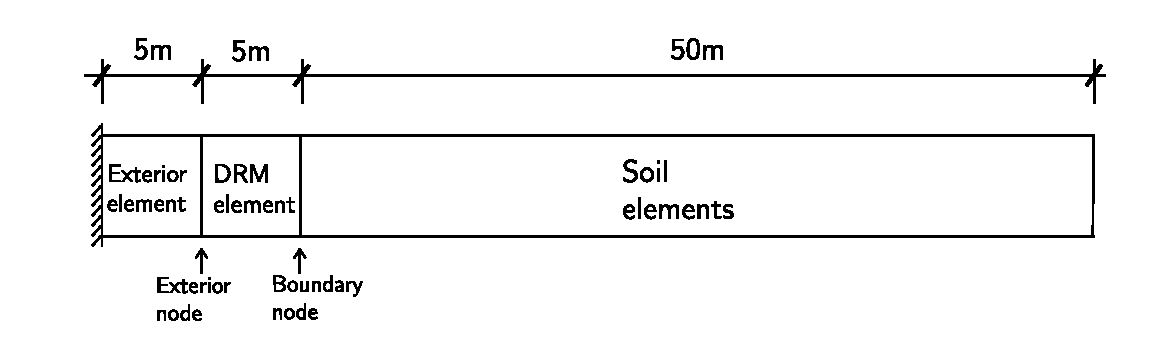
\includegraphics[width=18cm]{./Figure-files/_Chapter_Appendix_Illustrative_Examples/DRM_1D_descrp.pdf}
  \caption{1D DRM model.}
  \label{fig_Program_description_for_the_1D_DRM_model}
\end{figure}




%%%%%%%%%%%%%%%%%%%%%%%%%%%%%%%%%%%%%%%%%%%%%%%%%%%%%%%%%%%%%%%%%%%%
\paragraph{Numerical model:} ~


\begin{figure}[!htb]
  \centering
  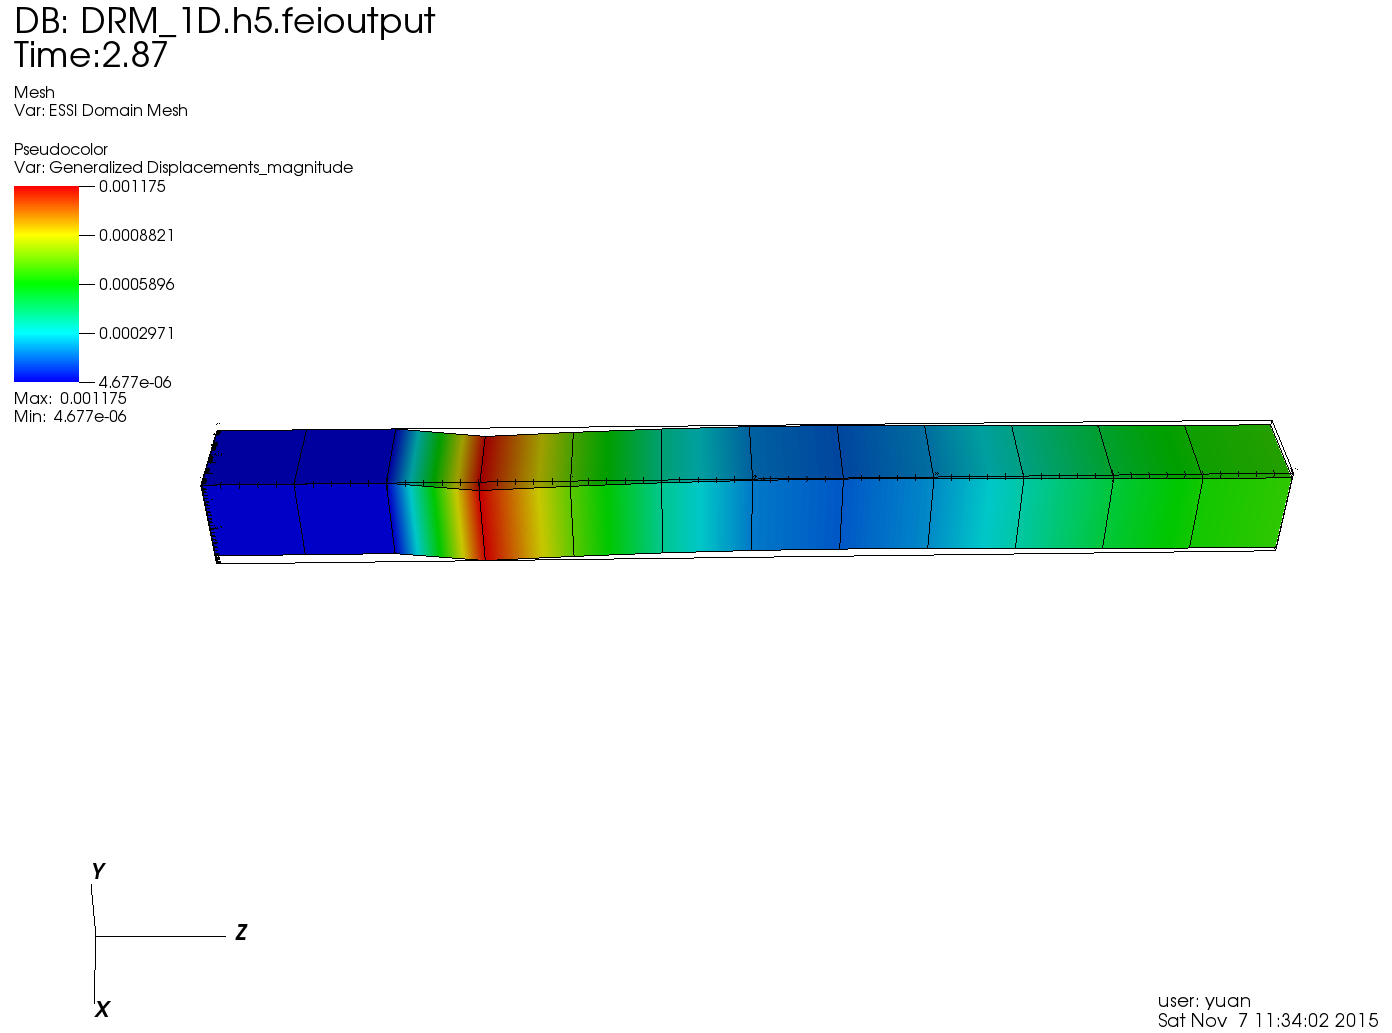
\includegraphics[width=15cm]{./Figure-files/_Chapter_Appendix_Illustrative_Examples/DRM_1D_result41.png}
  \caption{1D DRM model.}
  \label{fig Diagram for the 1D DRM model}
\end{figure}




%%%%%%%%%%%%%%%%%%%%%%%%%%%%%%%%%%%%%%%%%%%%%%%%%%%%%%%%%%%%%%%%%%%%
\paragraph{ESSI model fei file: } ~

%\lstinputlisting[frame=single]{../Figure-files/DRM_1D_script.fei}
\begin{lstlisting}
model name "DRM" ;

//Material for soil
add material # 1 type linear_elastic_isotropic_3d_LT
  mass_density = 2000*kg/m^3
  elastic_modulus = 1300*MPa
  poisson_ratio = 0.3;

//Material for DRM layer
add material # 2 type linear_elastic_isotropic_3d_LT
  mass_density = 2000*kg/m^3
  elastic_modulus = 1300*MPa
  poisson_ratio = 0.3;

//Material for exterior layer
add material # 3 type linear_elastic_isotropic_3d_LT
  mass_density = 2000*kg/m^3
  elastic_modulus = 1300*MPa
  poisson_ratio = 0.3;
//
add node # 1 at (  0.00*m,  0.00*m,  0.00*m) with 3 dofs;
add node # 2 at (  5.00*m,  0.00*m,  0.00*m) with 3 dofs;
add node # 3 at (  5.00*m,  5.00*m,  0.00*m) with 3 dofs;
add node # 4 at (  0.00*m,  5.00*m,  0.00*m) with 3 dofs;
add node # 5 at (  5.00*m,  0.00*m, 50.00*m) with 3 dofs;
add node # 6 at (  5.00*m,  0.00*m,  5.00*m) with 3 dofs;
...
...
add node # 52 at (  0.00*m, 5.00*m,  -5.00*m) with 3 dofs;

//
add element #       1 type 8NodeBrickLT with nodes( 1, 4, 3, 2, 24, 44, 34, 6) use material # 1;
add element #       2 type 8NodeBrickLT with nodes( 24, 44, 34, 6, 23, 43, 33, 7) use material # 1;
...
add element #      12 type 8NodeBrickLT with nodes( 48, 47, 45, 46, 52, 51, 49, 50) use material # 3;

//
fix node # 1 dofs uy ;
fix node # 1 dofs uz ;
fix node # 2 dofs uy ;
fix node # 2 dofs uz ;
fix node # 3 dofs uy ;
fix node # 3 dofs uz ;
fix node # 4 dofs uy ;
fix node # 4 dofs uz ;
...
fix node # 51 dofs ux ;


new loading stage "1D";
add domain reduction method loading #  1
  hdf5_file = "input.hdf5";

define algorithm With_no_convergence_check ;
define solver ProfileSPD;
define dynamic integrator Newmark with  gamma = 0.5  beta = 0.25;
simulate 999 steps using transient algorithm time_step = 0.01*s;

bye;
\end{lstlisting}

The ESSI model fei files for this example can be downloaded 
\href{https://github.com/BorisJeremic/Real-ESSI-Examples/blob/master/model_fei_file/8NodeBrick_DRM_1D/8NodeBrick_DRM_1D.tgz?raw=true}{here}.

The same model for this example with 27NodeBrickLT can be downloaded 
\href{https://github.com/BorisJeremic/Real-ESSI-Examples/blob/master/model_fei_file/27NodeBrick_DRM_1D/27NodeBrick_DRM_1D.tgz?raw=true}{here}.








%%%%%%%%%%%%%%%%%%%%%%%%%%%%%%%%%%%%%%%%%%%%%%%%%%%%%%%%%%%%%%%%%%%%
\paragraph{Long 1D DRM model 1000:1 } ~

To show the wave propagation explicitly, a long 1D model (1000:1) similar to the
1D DRM model above was made in this section.

The           model           description           is          same          to
Fig.(\ref{fig_Program_description_for_the_1D_DRM_model})  except  this model use
far more soil elements.

The general view is shown in Fig.(\ref{fig_Long_1D_DRM_model}) below.

\begin{figure}[!htb]
  \centering
  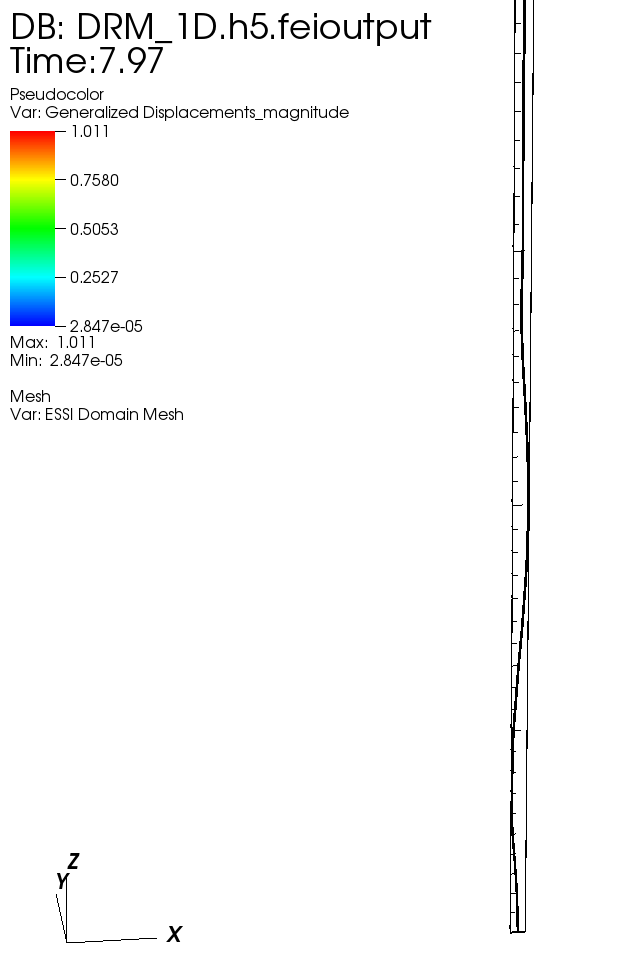
\includegraphics[width=10cm]{./Figure-files/_Chapter_Appendix_Illustrative_Examples/long_DRM_full.png}
  \caption{Long 1D DRM model}
  \label{fig_Long_1D_DRM_model}
\end{figure}

There is still now outgoing waves at the exterior layers, which is shown in Fig(\ref{fig_Long_1D_DRM_model_exterior_layer}).
\begin{figure}[!htb]
  \centering
  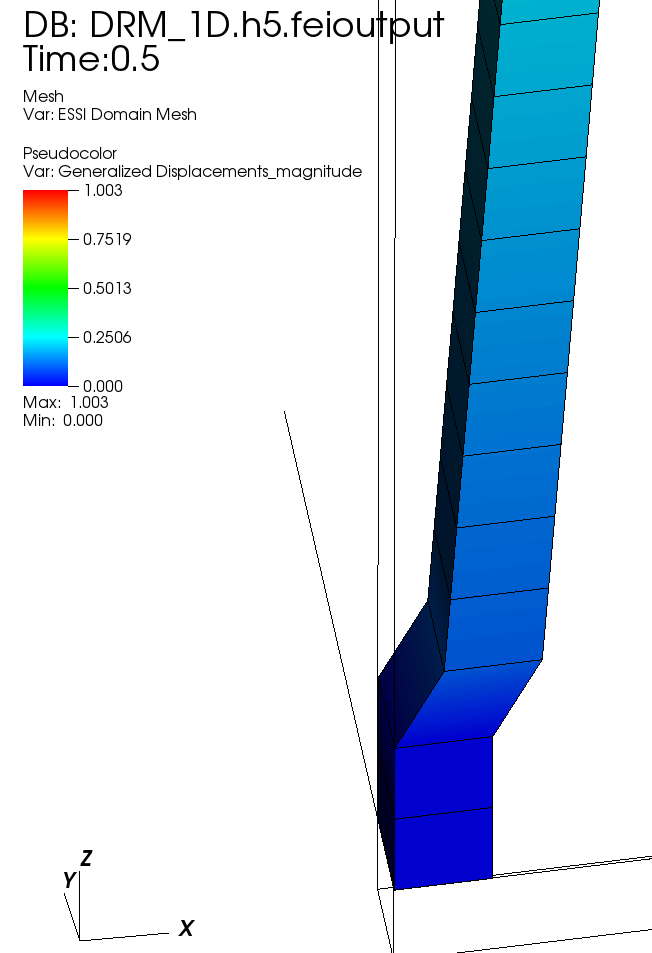
\includegraphics[width=5cm]{./Figure-files/_Chapter_Appendix_Illustrative_Examples/long_DRM_part.png}
  \caption{Long 1D DRM model: exterior layer}
  \label{fig_Long_1D_DRM_model_exterior_layer}
\end{figure}


The ESSI model fei files for this example can be downloaded 
\href{https://github.com/BorisJeremic/Real-ESSI-Examples/blob/master/model_fei_file/8NodeBrick_DRM_1D_long/8NodeBrick_DRM_1D_long.tgz?raw=true}{here}.

The results can also be seen from this 
\href{http://sokocalo.engr.ucdavis.edu/~jeremic/lecture_notes_online_material/_Chapter_Applications_Earthquake_Soil_Structure_Interaction_General_Aspects/Animation_DRM_1D.mp4}{video}.














%%%%%%%%%%%%%%%%%%%%%%%%%%%%%%%%%%%%%%%%%%%%%%%%%%%%%%%%%%%%%%%%%%%%
\clearpage  
% add new page to avoid the figure confusion with previous section
%%%%%%%%%%%%%%%%%%%%%%%%%%%%%%%%%%%%%%%%%%%%%%%%%%%%%%%%%%%%%%%%%%%%












%%%%%%%%%%%%%%%%%%%%%%%%%%%%%%%%%%%%%%%%%%%%%%%%%%%%%%%%%%%%%%%%%%%%%%%%%%%%%%%%
%%%%%%%%%%%%%%%%%%%%%%%%%%%%%%%%%%%%%%%%%%%%%%%%%%%%%%%%%%%%%%%%%%%%%%%%%%%%%%%%
%%%%%%%%%%%%%%%%%%%%%%%%%%%%%%%%%%%%%%%%%%%%%%%%%%%%%%%%%%%%%%%%%%%%%%%%%%%%%%%%
%%%%%%%%%%%%%%%%%%%%%%%%%%%%%%%%%%%%%%%%%%%%%%%%%%%%%%%%%%%%%%%%%%%%%%%%%%%%%%%%
%%%%%%%%%%%%%%%%%%%%%%%%%%%%%%%%%%%%%%%%%%%%%%%%%%%%%%%%%%%%%%%%%%%%%%%%%%%%%%%%
\section{Three Dimensional DRM Model}

%%%%%%%%%%%%%%%%%%%%%%%%%%%%%%%%%%%%%%%%%%%%%%%%%%%%%%%%%%%%%%%%%%%%
\paragraph{Problem description:} ~

As shown in Fig.(\ref{fig The diagram for Domain Reduction Method DRM }), the DRM layer is used to add the earthquake motion. 


\begin{figure}[!htb]
  \centering
  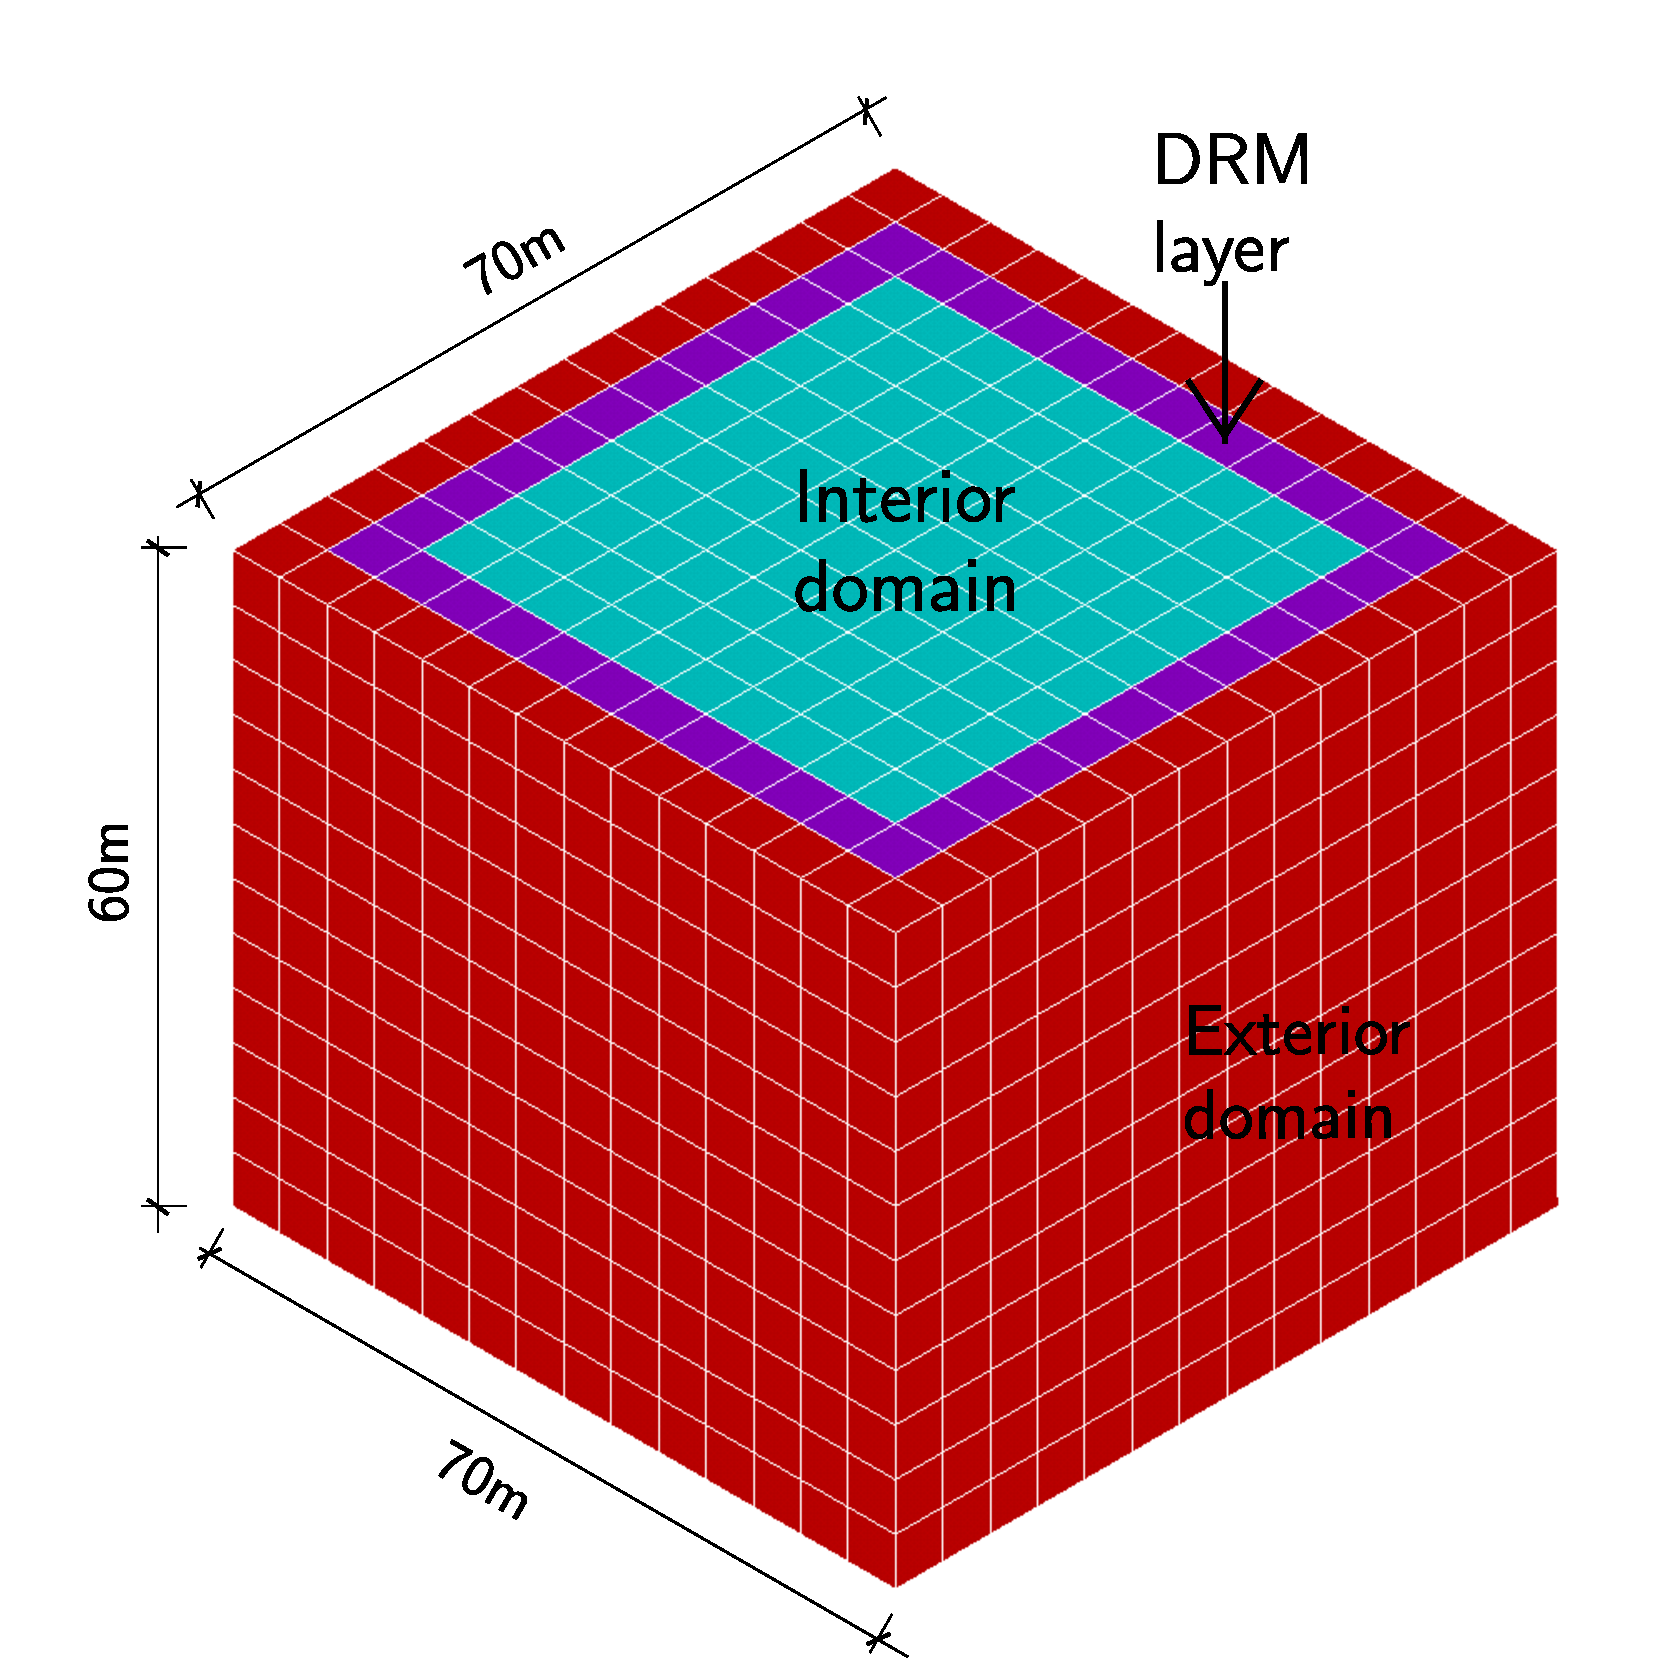
\includegraphics[width=10cm]{./Figure-files/_Chapter_Appendix_Illustrative_Examples/DRM_3D_descp_3.pdf}
  \caption{The diagram for 3D Domain Reduction Method example.}
  \label{fig The diagram for Domain Reduction Method DRM }
\end{figure}


% In 2D, the DRM model is shown in Fig.(\ref{fig The diagram for Domain Reduction Method DRM 2d }). 
% \begin{figure}[!htb]
%   \centering
%   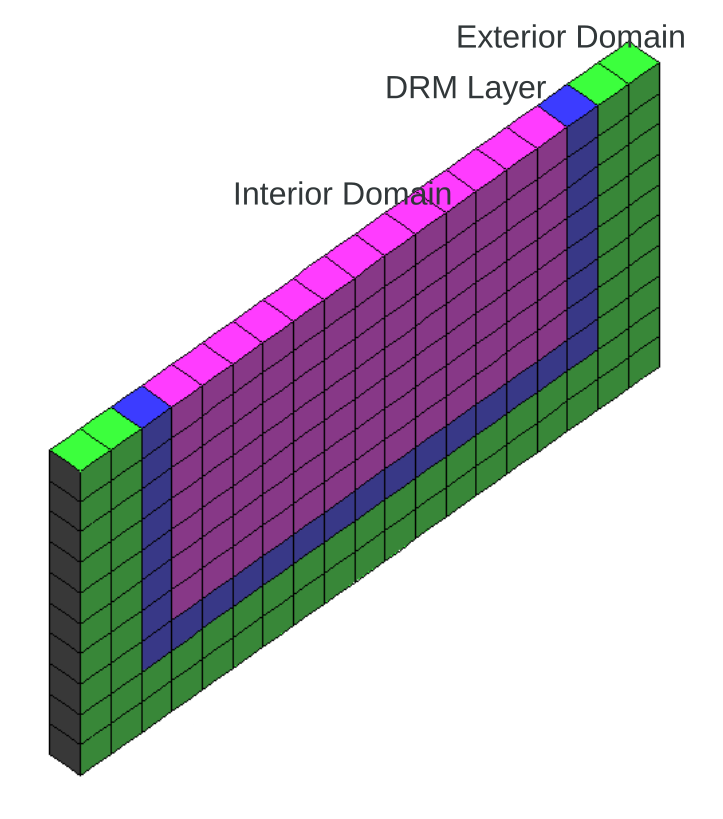
\includegraphics[width=10cm]{../Figure-files/DRM_diagram_2d.png}
%   \caption{The diagram for 2D Domain Reduction Method (DRM) }
%   \label{fig The diagram for Domain Reduction Method DRM 2d }
% \end{figure}




%%%%%%%%%%%%%%%%%%%%%%%%%%%%%%%%%%%%%%%%%%%%%%%%%%%%%%%%%%%%%%%%%%%%
\paragraph{Numerical result:} ~

\begin{figure}[!htb]
  \centering
  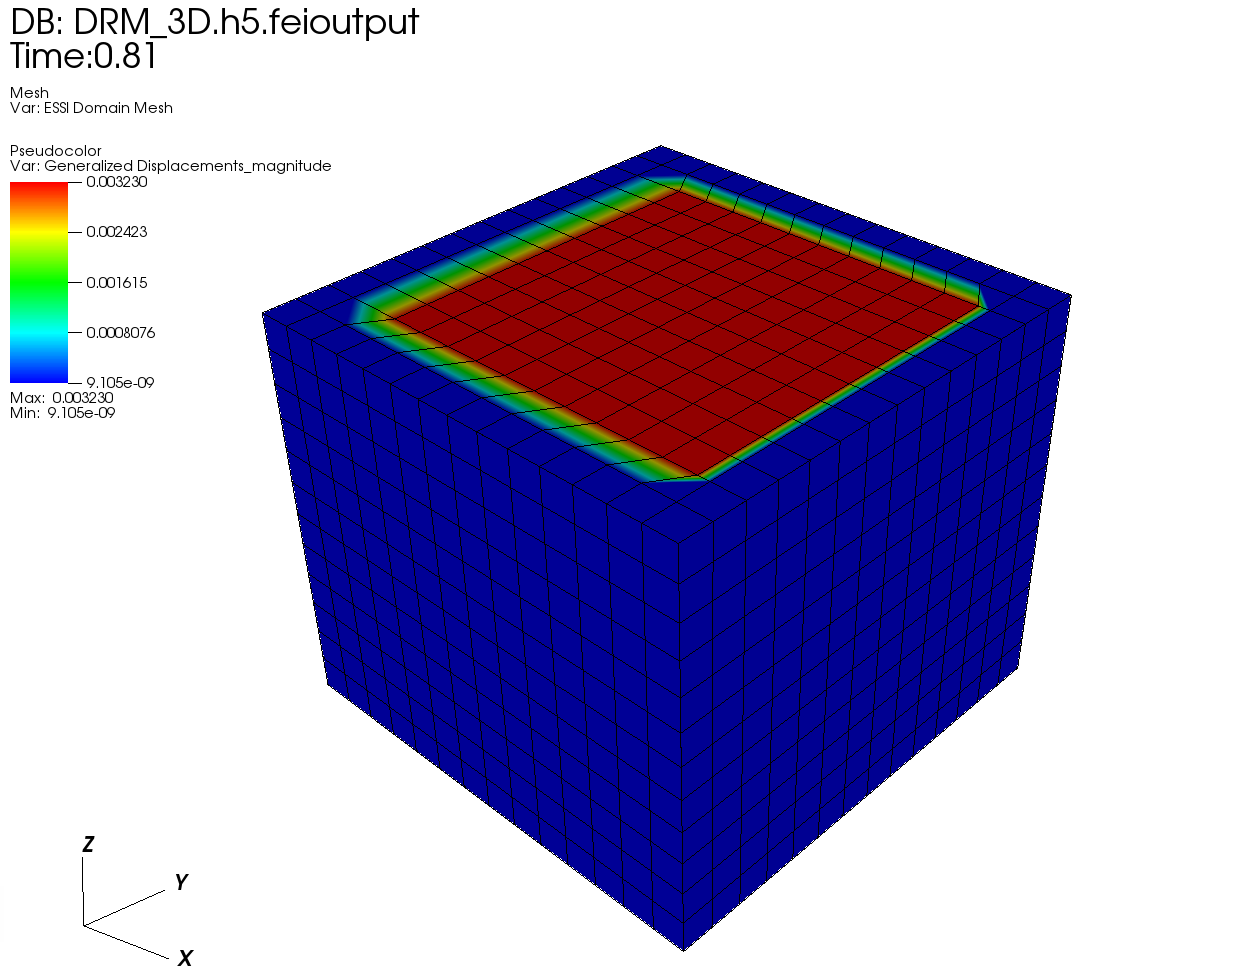
\includegraphics[width=15cm]{./Figure-files/_Chapter_Appendix_Illustrative_Examples/3d_drm_result429.png}
  \caption{Diagram for the 3D DRM model.}
  \label{fig Diagram for the 3D DRM model}
\end{figure}


%%%%%%%%%%%%%%%%%%%%%%%%%%%%%%%%%%%%%%%%%%%%%%%%%%%%%%%%%%%%%%%%%%%%
\paragraph{ESSI model fei file: } ~

%\lstinputlisting[frame=single]{../Figure-files/DRM_3D_script.fei}
\begin{lstlisting}
model name "DRM" ;

//Material for soil
add material # 1 type linear_elastic_isotropic_3d_LT
  mass_density = 2000*kg/m^3
  elastic_modulus = 1300*MPa
  poisson_ratio = 0.3;

//Material for DRM layer
add material # 2 type linear_elastic_isotropic_3d_LT
  mass_density = 2000*kg/m^3
  elastic_modulus = 1300*MPa
  poisson_ratio = 0.3;

//Material for exterior layer
add material # 3 type linear_elastic_isotropic_3d_LT
  mass_density = 2000*kg/m^3
  elastic_modulus = 1300*MPa
  poisson_ratio = 0.3;

//
add node #  1 at (   0.00*m,   0.00*m,   0.00*m) with 3 dofs;
add node #  2 at (   50.00*m,   0.00*m,   0.00*m) with 3 dofs;
add node #  3 at (   5.00*m,   0.00*m,   0.00*m) with 3 dofs;
add node #  4 at (   10.00*m,   0.00*m,   0.00*m) with 3 dofs;
add node #  5 at (   15.00*m,   0.00*m,   0.00*m) with 3 dofs;
add node #  6 at (   20.00*m,   0.00*m,   0.00*m) with 3 dofs;
add node #  7 at (   25.00*m,   0.00*m,   0.00*m) with 3 dofs;
...
...
add node # 2925 at (   55.00*m,   55.00*m,   -5.00*m) with 3 dofs;

//
add element #  1 type 8NodeBrickLT with nodes(  1,  40,  41,  3, 150, 441, 603, 151) use material # 1;
add element #  2 type 8NodeBrickLT with nodes(  3,  41,  50,  4, 151, 603, 684, 160) use material # 1;
...
add element # 2352 type 8NodeBrickLT with nodes( 2925, 2924, 2922, 2923, 2921, 2920, 2918, 2919) use material # 3;

//
fix node #  1332 dofs all  ;
fix node #  1334 dofs all  ;
...
...
fix node #  2924 dofs all  ;

new loading stage "3D";
add domain reduction method loading #  1
  hdf5_file = "input.hdf5";

define algorithm With_no_convergence_check ;
define solver ProfileSPD;
define dynamic integrator Newmark with  gamma = 0.5  beta = 0.25;

simulate 999 steps using transient algorithm  time_step = 0.01*s;

bye;
\end{lstlisting}

The    ESSI   model   fei   files   for   this   example   can   be   downloaded
\href{https://github.com/BorisJeremic/Real-ESSI-Examples/blob/master/model_fei_file/8NodeBrick_DRM_3D/8NodeBrick_DRM_3D.tgz?raw=true}{here}.

The   same   model  for  this  example  with  27NodeBrickLT  can  be  downloaded
\href{https://github.com/BorisJeremic/Real-ESSI-Examples/blob/master/model_fei_file/27NodeBrick_DRM_3D/27NodeBrick_DRM_3D.tgz?raw=true}{here}.






%%%%%%%%%%%%%%%%%%%%%%%%%%%%%%%%%%%%%%%%%%%%%%%%%%%%%%%%%%%%%%%%%%%%%%%%%%%%%%%%
%%%%%%%%%%%%%%%%%%%%%%%%%%%%%%%%%%%%%%%%%%%%%%%%%%%%%%%%%%%%%%%%%%%%%%%%%%%%%%%%
%%%%%%%%%%%%%%%%%%%%%%%%%%%%%%%%%%%%%%%%%%%%%%%%%%%%%%%%%%%%%%%%%%%%%%%%%%%%%%%%
%%%%%%%%%%%%%%%%%%%%%%%%%%%%%%%%%%%%%%%%%%%%%%%%%%%%%%%%%%%%%%%%%%%%%%%%%%%%%%%%
%%%%%%%%%%%%%%%%%%%%%%%%%%%%%%%%%%%%%%%%%%%%%%%%%%%%%%%%%%%%%%%%%%%%%%%%%%%%%%%%
%%%%%%%%%%%%%%%%%%%%%%%%%%%%%%%%%%%%%%%%%%%%%%%%%%%%%%%%%%%%%%%%%%%%
%%%%%%%%%%%%%%%%%%%%%%%%%%%%%%%%%%%%%%%%%%%%%%%%%%%%%%%%%%%%%%%%%%%%
\section{ShearBeam Element for Pisano Materials}

%%%%%%%%%%%%%%%%%%%%%%%%%%%%%%%%%%%%%%%%%%%%%%%%%%%%%%%%%%%%%%%%%%%%
\paragraph{Problem description:} ~

In  the  element  type  "ShearBeamLT",  only  one Gauss point exists. 
ShearBeamLT  element  was used here to test the Pisan{\'o}
material model.

Vertical    force    $F_z$   was used to apply confinement to the element. Then,
cyclic force  $F_x$ is  used to load. 
point.

\begin{figure}[!htb]
  \centering
  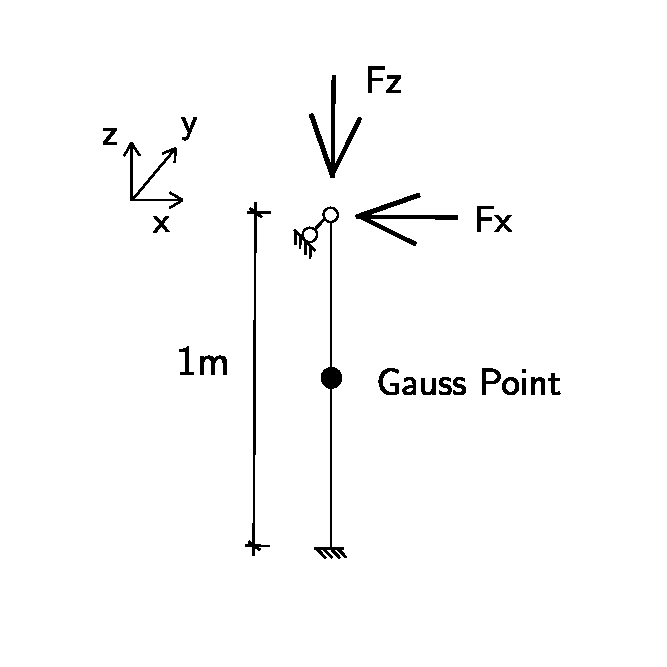
\includegraphics[width=10cm]{./Figure-files/_Chapter_Appendix_Illustrative_Examples/pisano_descrip.pdf}
  \caption{ShearBeam element.}
  \label{fig_ShearBeam}
\end{figure}



%%%%%%%%%%%%%%%%%%%%%%%%%%%%%%%%%%%%%%%%%%%%%%%%%%%%%%%%%%%%%%%%%%%%
\paragraph{Results} ~

Resulting stress-strain relationship is shown in Fig.(\ref{fig_ShearBeam_result}). 

\begin{figure}[!htb]
  \centering
  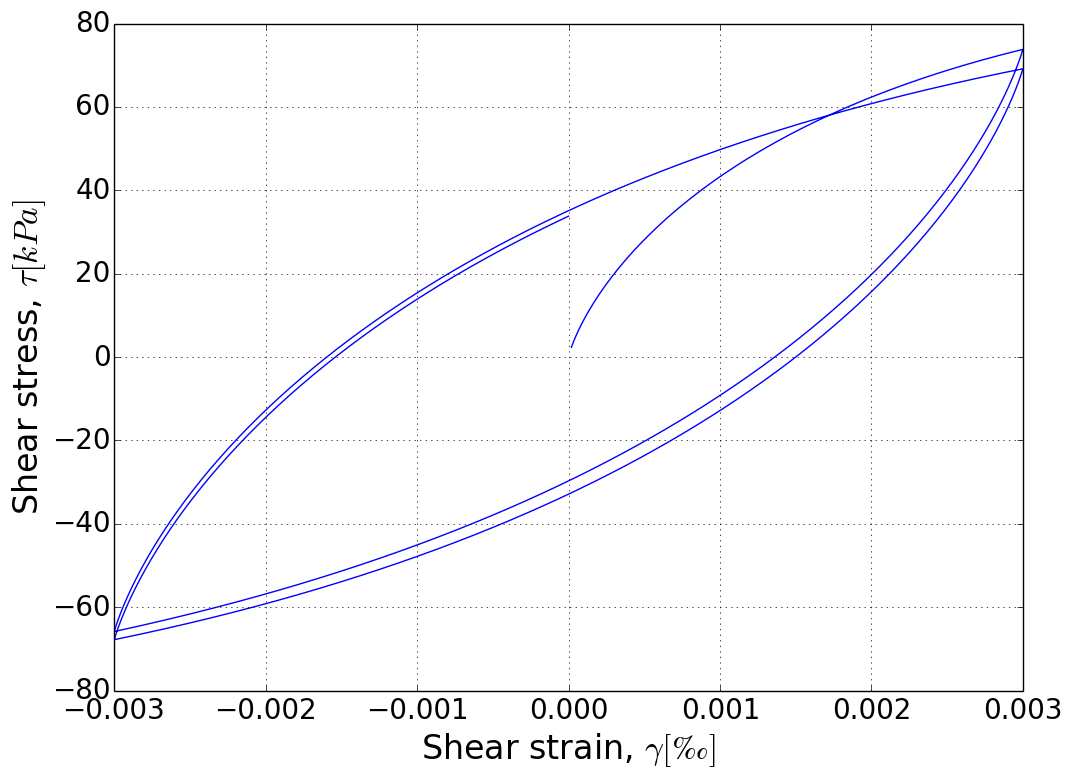
\includegraphics[width=12cm]{./Figure-files/_Chapter_Appendix_Illustrative_Examples/pisanoLT_test01.png}
  \caption{Shear stress-strain response.}
  \label{fig_ShearBeam_result}
\end{figure}

%%%%%%%%%%%%%%%%%%%%%%%%%%%%%%%%%%%%%%%%%%%%%%%%%%%%%%%%%%%%%%%%%%%%
\paragraph{ESSI model fei file: } ~

%\lstinputlisting[frame=single]{../Figure-files/2test_pisano_01.fei}
\begin{lstlisting}
model name "pisanoLT";

add node # 1 at (0*m,0*m,0*m)  with 3 dofs;
add node # 2 at (0*m,0*m,1*m)  with 3 dofs;

fix node # 1 dofs all;
fix node # 2 dofs uy;

add material # 1 type New_PisanoLT
 mass_density = 2000*kg/m^3
 elastic_modulus_1atm =  325*MPa  poisson_ratio =  0.3
 M_in =  1.4   kd_in =  0.0  xi_in =  0.0  h_in =  700  m_in =  0.7
 initial_confining_stress =  0*kPa n_in = 0  a_in = 0.0  eplcum_cr_in = 1e-6;

add element # 1 type ShearBeamLT with nodes (1, 2) \
     cross_section = 1*m^2 use material # 1;

new loading stage "confinement";

add load # 1 to node # 2 type linear Fz = -200*kN;
define load factor increment 0.01;
define algorithm With_no_convergence_check ;
define solver  UMFPack;
simulate 100 steps using static algorithm;

new loading stage "test01";
gamma_max = 3e-3;
add imposed motion # 2 to node # 2 dof ux
 displacement_scale_unit = gamma_max*m displacement_file = "input_sine.txt"
 velocity_scale_unit = gamma_max*m/s velocity_file = "input_sine.txt"
 acceleration_scale_unit = gamma_max*m/s^2 acceleration_file = "input_sine.txt";

define load factor increment 0.0005;
define algorithm With_no_convergence_check;
define solver  UMFPack;
simulate 2000 steps using static algorithm;

bye;
\end{lstlisting}

The    ESSI   model   fei   files   for   this   example   can   be   downloaded
\href{https://github.com/BorisJeremic/Real-ESSI-Examples/blob/master/model_fei_file/shearbeam_pisano_plastic/shearbeam_pisano_plastic.tgz?raw=true}{here}.


























%%%%%%%%%%%%%%%%%%%%%%%%%%%%%%%%%%%%%%%%%%%%%%%%%%%%%%%%%%%%%%%%%%%%%%%%%%%%%%%%
%%%%%%%%%%%%%%%%%%%%%%%%%%%%%%%%%%%%%%%%%%%%%%%%%%%%%%%%%%%%%%%%%%%%%%%%%%%%%%%%
%%%%%%%%%%%%%%%%%%%%%%%%%%%%%%%%%%%%%%%%%%%%%%%%%%%%%%%%%%%%%%%%%%%%%%%%%%%%%%%%
%%%%%%%%%%%%%%%%%%%%%%%%%%%%%%%%%%%%%%%%%%%%%%%%%%%%%%%%%%%%%%%%%%%%%%%%%%%%%%%%
%%%%%%%%%%%%%%%%%%%%%%%%%%%%%%%%%%%%%%%%%%%%%%%%%%%%%%%%%%%%%%%%%%%%%%%%%%%%%%%%
%%%%%%%%%%%%%%%%%%%%%%%%%%%%%%%%%%%%%%%%%%%%%%%%%%%%%%%%%%%%%%%%%%%%
%%%%%%%%%%%%%%%%%%%%%%%%%%%%%%%%%%%%%%%%%%%%%%%%%%%%%%%%%%%%%%%%%%%%
\section{8NodeBrickLT Element for Drucker Prager Armstrong Federick Materials }

%%%%%%%%%%%%%%%%%%%%%%%%%%%%%%%%%%%%%%%%%%%%%%%%%%%%%%%%%%%%%%%%%%%%
\paragraph{Problem description:} ~

This example is used to test the materials properties, such as G/Gmax against strains. The element type is 8NodeBrickLT. And there are two stages of loading. The first loading stage is confinement and the second loading stage is shearing. 

The boundary condition is specially designed such that each Gauss point has the same stress state. 





%%%%%%%%%%%%%%%%%%%%%%%%%%%%%%%%%%%%%%%%%%%%%%%%%%%%%%%%%%%%%%%%%%%%
\paragraph{Results} ~

Resulting stress-strain relationship is shown in Fig.(\ref{fig_8nodebrick_result}). 

\begin{figure}[!htb]
  \centering
  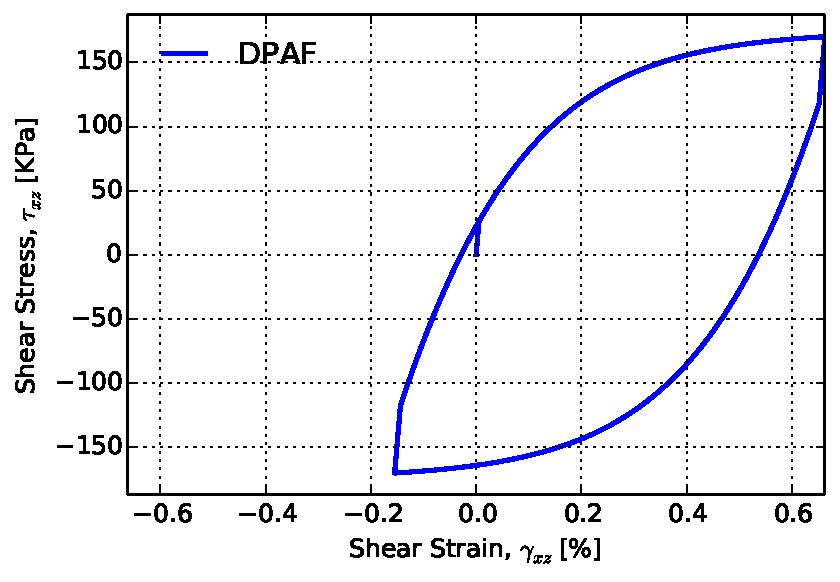
\includegraphics[width=12cm]{./Figure-files/_Chapter_Appendix_Illustrative_Examples/drucker_prager_armstrong_federick.pdf}
  \caption{Shear stress-strain response.}
  \label{fig_8nodebrick_result}
\end{figure}

%%%%%%%%%%%%%%%%%%%%%%%%%%%%%%%%%%%%%%%%%%%%%%%%%%%%%%%%%%%%%%%%%%%%
\paragraph{ESSI model fei file: } ~

%\lstinputlisting[frame=single]{../Figure-files/2test_pisano_01.fei}

\begin{lstlisting}
// Drucker Prager Armstrong Frederick
// This model is created by Jose.
model name "druckeraf";

// Parameters:
phi   = 5;
ha      = 1000;
cr      = 973;
gam        = 0.01;
Ncyc       = 5;
Nsteps     = 1000;
H=1;
vp=1000*m/s;
vs=500*m/s; 
rho=2000*kg/m^3;
p0 = 250*kPa;
G = rho*vs^2;
M = rho*vp^2;

//From wiki (https://en.wikipedia.org/wiki/Elastic_modulus)
E = G*(3*M-4*G)/(M-G);
nu = (M-2*G)/(2*M-2*G);

K0 = 1.0;
phirad = pi*phi/180;
M = 6*sin(phirad)/(3-sin(phirad));

// Define the material:
add material # 1 type DruckerPragerArmstrongFrederickLT
    mass_density = 0*kg/m^3 
    elastic_modulus =  E
    poisson_ratio =  nu
    druckerprager_k = M
    armstrong_frederick_ha = ha*Pa 
    armstrong_frederick_cr = cr*Pa
    isotropic_hardening_rate =  0*E
    initial_confining_stress = 1*Pa;

// define the node:
add node # 1 at (0*m,0*m,1*m)  with 3 dofs;
add node # 2 at (1*m,0*m,1*m)  with 3 dofs;
add node # 3 at (1*m,1*m,1*m)  with 3 dofs;
add node # 4 at (0*m,1*m,1*m)  with 3 dofs;

add node # 5 at (0*m,0*m,0*m)  with 3 dofs;
add node # 6 at (1*m,0*m,0*m)  with 3 dofs;
add node # 7 at (1*m,1*m,0*m)  with 3 dofs;
add node # 8 at (0*m,1*m,0*m)  with 3 dofs;

// add equal degree of freedom in three directions
add constraint equal dof with master node # 2 and slave node # 3 dof to constrain ux;
add constraint equal dof with master node # 2 and slave node # 6 dof to constrain ux;
add constraint equal dof with master node # 2 and slave node # 7 dof to constrain ux;

add constraint equal dof with master node # 3 and slave node # 4 dof to constrain uy;
add constraint equal dof with master node # 3 and slave node # 8 dof to constrain uy;
add constraint equal dof with master node # 3 and slave node # 7 dof to constrain uy;

add constraint equal dof with master node # 1 and slave node # 2 dof to constrain uz;
add constraint equal dof with master node # 1 and slave node # 3 dof to constrain uz;
add constraint equal dof with master node # 1 and slave node # 4 dof to constrain uz;

// Define the element.
add element # 1 type 8NodeBrickLT with nodes (1, 2,3 , 4, 5, 6,7, 8) use material # 1;

new loading stage "confinement";
fix node # 1 dofs ux uy;
fix node # 2 dofs uy;
fix node # 4 dofs ux;

fix node # 5 dofs ux uy uz;
fix node # 6 dofs uy uz;
fix node # 7 dofs uz;
fix node # 8 dofs ux uz;

sigma_z = -3*p0/(1+2*K0);
sigma_x = K0*sigma_z;
sigma_y = K0*sigma_z;

//Z-face
add load # 1 to node # 1 type linear  Fz = sigma_z*m^2/4;
add load # 2 to node # 2 type linear  Fz = sigma_z*m^2/4;
add load # 3 to node # 3 type linear  Fz = sigma_z*m^2/4;
add load # 4 to node # 4 type linear  Fz = sigma_z*m^2/4;

//X-face
add load # 5 to node # 2 type linear  Fx = sigma_x*m^2/4;
add load # 6 to node # 6 type linear  Fx = sigma_x*m^2/4;
add load # 7 to node # 7 type linear  Fx = sigma_x*m^2/4;
add load # 8 to node # 3 type linear  Fx = sigma_x*m^2/4;

add load # 9 to node # 3 type linear   Fy = sigma_y*m^2/4;
add load # 10 to node # 7 type linear  Fy = sigma_y*m^2/4;
add load # 11 to node # 8 type linear  Fy = sigma_y*m^2/4;
add load # 12 to node # 4 type linear  Fy = sigma_y*m^2/4;

Nsteps_static=100;
define load factor increment 1/Nsteps_static;

define solver  UMFPack;
define convergence test Norm_Displacement_Increment  
    tolerance =  1e-6
    maximum_iterations =  100
    verbose_level = 4;
define algorithm Newton ;

define NDMaterialLT constitutive integration algorithm Euler_One_Step
    yield_function_relative_tolerance =  0.002
    stress_relative_tolerance =  0.002
    maximum_iterations = 1000;

simulate Nsteps_static steps using static algorithm;


new loading stage "shearing";
compute reaction forces;
add load # 13 to node # 1 type from_reactions;
add load # 14 to node # 4 type from_reactions;

free node # 1 dofs ux;
free node # 4 dofs ux;
fix node # 3 dofs uy;
fix node # 6 dofs ux;
fix node # 7 dofs ux uy;
fix node # 8 dofs uy;

add constraint equal dof with master node # 1 and slave node # 3 dof to constrain ux;
add constraint equal dof with master node # 1 and slave node # 4 dof to constrain ux;
add constraint equal dof with master node # 1 and slave node # 2 dof to constrain ux;
remove constraint equaldof node # 6;
remove constraint equaldof node # 7;
remove constraint equaldof node # 8;

n = 1;
while(n<=1)
{
    add load # 14+n to node # n type path_time_series 
     Fx = 170.*kN 
     series_file = "path.txt";        
    n+=1;
}

define load factor increment 1/Nsteps;

define solver  UMFPack;
define convergence test Norm_Displacement_Increment  
    tolerance =  1e-5
    maximum_iterations =  100
    verbose_level = 4;
define algorithm Newton ;

define NDMaterialLT constitutive integration algorithm Euler_One_Step
    yield_function_relative_tolerance =  0.0002
    stress_relative_tolerance =  0.002
    maximum_iterations = 1000;

simulate Ncyc*Nsteps steps using static algorithm;

bye;    
\end{lstlisting}

The    ESSI   model   fei   files   for   this   example   can   be   downloaded
\href{https://github.com/BorisJeremic/Real-ESSI-Examples/blob/master/model_fei_file/shearbeam_pisano_plastic8NodeBrickLT_DruckerPragerArmstrongFrederick/8NodeBrickLT_DruckerPragerArmstrongFrederick.tgz?raw=true}{here}.







































%%%%%%%%%%%%%%%%%%%%%%%%%%%%%%%%%%%%%%%%%%%%%%%%%%%%%%%%%%%%%%%%%%%%%%%%%%%%%%%%
%%%%%%%%%%%%%%%%%%%%%%%%%%%%%%%%%%%%%%%%%%%%%%%%%%%%%%%%%%%%%%%%%%%%%%%%%%%%%%%%
%%%%%%%%%%%%%%%%%%%%%%%%%%%%%%%%%%%%%%%%%%%%%%%%%%%%%%%%%%%%%%%%%%%%%%%%%%%%%%%%
%%%%%%%%%%%%%%%%%%%%%%%%%%%%%%%%%%%%%%%%%%%%%%%%%%%%%%%%%%%%%%%%%%%%%%%%%%%%%%%%
%%%%%%%%%%%%%%%%%%%%%%%%%%%%%%%%%%%%%%%%%%%%%%%%%%%%%%%%%%%%%%%%%%%%%%%%%%%%%%%%
%%%%%%%%%%%%%%%%%%%%%%%%%%%%%%%%%%%%%%%%%%%%%%%%%%%%%%%%%%%%%%%%%%%%
%%%%%%%%%%%%%%%%%%%%%%%%%%%%%%%%%%%%%%%%%%%%%%%%%%%%%%%%%%%%%%%%%%%%

\newpage
\section{Elastic Beam Element under Dynamic Loading} ~ 
\subsection{Simulate the cantilever by 1 elastic beam element} 
\paragraph{Problem description:} ~

\begin{itemize}
  \item Structure size

    Structure Length=1m, width=0.2m, height=0.2m.

  \item Element size

    Element length=1m, width=0.2m, height=0.2m.
\end{itemize}

\begin{figure}[!htb]
  \centering
  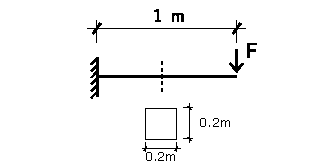
\includegraphics[width=12cm]{./Figure-files/_Chapter_Appendix_Illustrative_Examples/cantilever.pdf}
  \caption{The cantilever model}
  \label{fig-canti_1beam}
\end{figure}


\paragraph{ESSI model fei file: } ~

\begin{lstlisting}
model name "beam_1element" ;

// add node
add node #  1 at (   0.0*m ,    0.0*m,     0.0*m)  with 6 dofs;
add node #  2 at (   1.0*m ,    0.0*m,     0.0*m)  with 6 dofs;
  
// Geometry: width and height
b=0.2*m;
h=0.2*m;

// Materials: properties
natural_period    = 1*s;        
natural_frequency  = 2*pi/natural_period;
elastic_constant  = 1e9*N/m^2; 
I=b*h^3/12.0;
A=b*h;
L=1*m;
rho   = (1.8751)^4*elastic_constant*I/(natural_frequency^2*L^4*A);
possion_ratio=0.3;

// add elements
add element # 1 type beam_elastic with nodes (1,2) 
  cross_section =   b*h 
  elastic_modulus =  elastic_constant
  shear_modulus =  elastic_constant/2/(1+possion_ratio)
  torsion_Jx =  0.33*b*h^3
  bending_Iy =  b*h^3/12
  bending_Iz =  b*h^3/12
  mass_density = rho
  xz_plane_vector = ( 1, 0, 1) 
  joint_1_offset = (0*m, 0*m, 0*m) 
  joint_2_offset = (0*m, 0*m, 0*m);

// add boundary condition
fix node #      1 dofs all;

// // ----------------------------------------------------------------------------
// // --slowLoading---------------------------------------------------------------
// // add the 1 Newton load in 180 seconds. 
// // ----------------------------------------------------------------------------
// new loading stage "slowLoading";
// add load # 1 to node # 2 type path_time_series 
//  Fz =  1.*N
//  series_file = "slowLoading.txt" ;
// define dynamic integrator Newmark with gamma = 0.5 beta = 0.25;
// define algorithm With_no_convergence_check ;
// define solver ProfileSPD;
// simulate 2000 steps using transient algorithm 
//  time_step = 0.1*s;

// // ----------------------------------------------------------------------------
// // --fastLoading---------------------------------------------------------------
// // add the 1 Newton load in 0.6 seconds.
// // ----------------------------------------------------------------------------
// remove load # 1;
// new loading stage "fastLoading";
// add load # 2 to node # 2 type path_time_series 
//  Fz =  1.*N
//  series_file = "fastLoading.txt" ;
// define dynamic integrator Newmark with gamma = 0.5 beta = 0.25;
// define algorithm With_no_convergence_check ;
// define solver ProfileSPD;
// simulate 1000 steps using transient algorithm 
//  time_step = 0.01*s;

// // ----------------------------------------------------------------------------
// // --freeVibration-------------------------------------------------------------
// // add a load and then release to free vibration
// // ----------------------------------------------------------------------------
// remove load # 2;
new loading stage "freeVibration";
add load # 3 to node # 2 type path_time_series 
  Fz =  1.*N
  series_file = "freeVibration.txt" ;
define dynamic integrator Newmark with gamma = 0.5 beta = 0.25;
define algorithm With_no_convergence_check ;
define solver ProfileSPD;
simulate 2000 steps using transient algorithm 
  time_step = 0.01*s;

bye;
\end{lstlisting}

\paragraph{Displacement results against time series} ~

\begin{figure}[!htb]
  \centering
  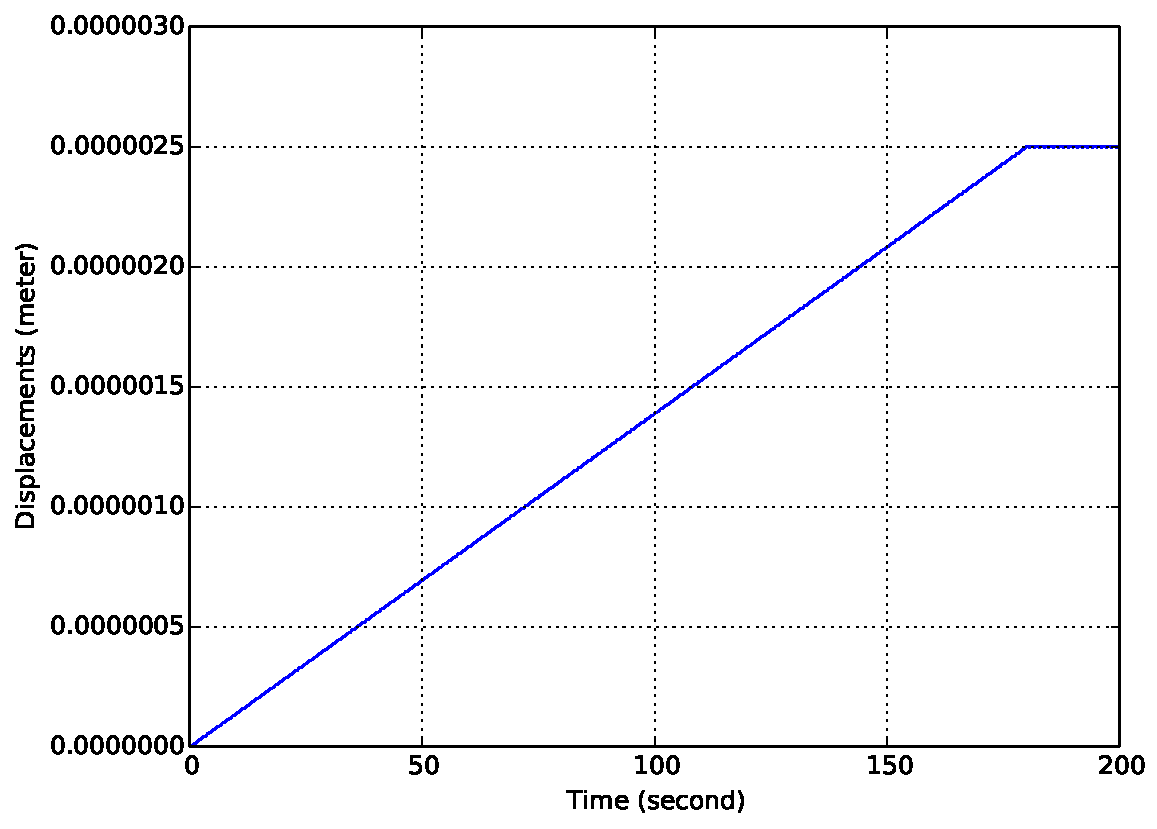
\includegraphics[width=12cm]{./Figure-files/_Chapter_Appendix_Illustrative_Examples/beam-1element-slowLoading.pdf}
  \caption{Simulate the cantilever by 1 elastic beam element under the slow loading}
  \label{fig_beam1_slow}
\end{figure}


\begin{figure}[!htb]
  \centering
  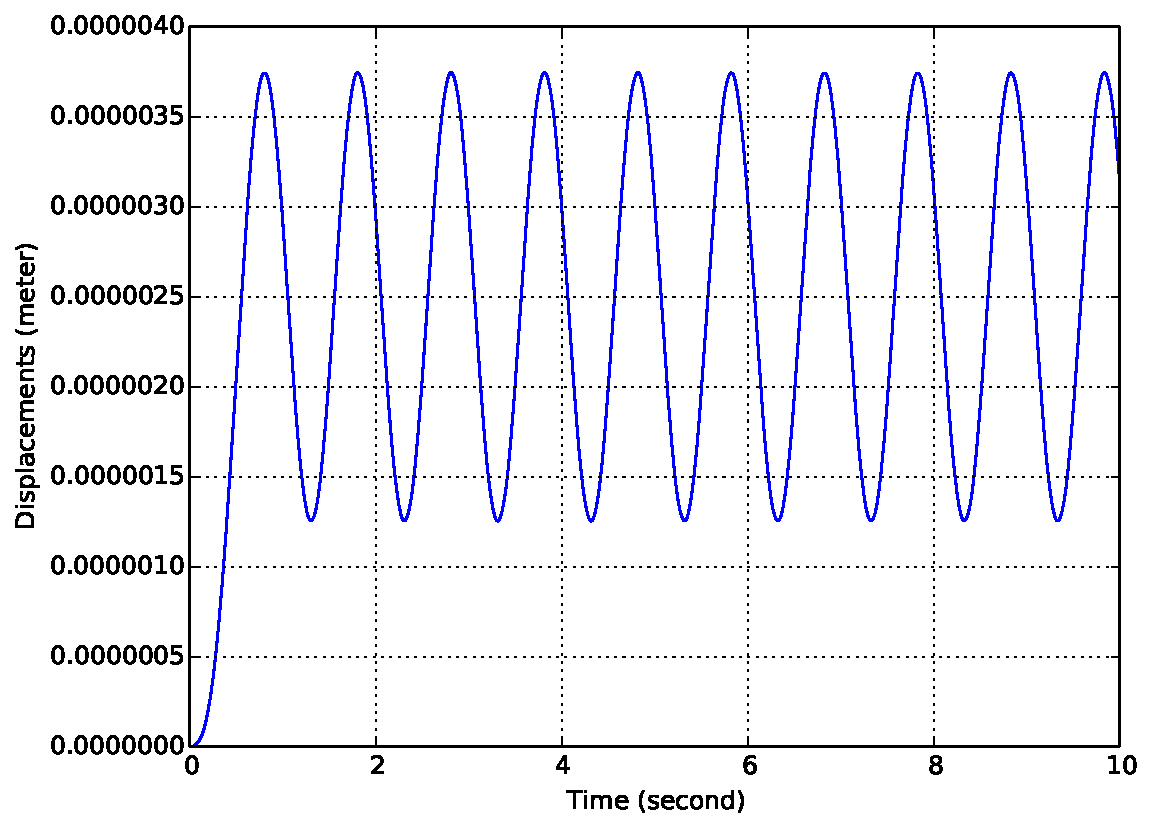
\includegraphics[width=12cm]{./Figure-files/_Chapter_Appendix_Illustrative_Examples/beam-1element-fastLoading.pdf}
  \caption{Simulate the cantilever by 1 elastic beam element under the fast loading}
  \label{fig_beam1_fast}
\end{figure}

\begin{figure}[!htb]
  \centering
  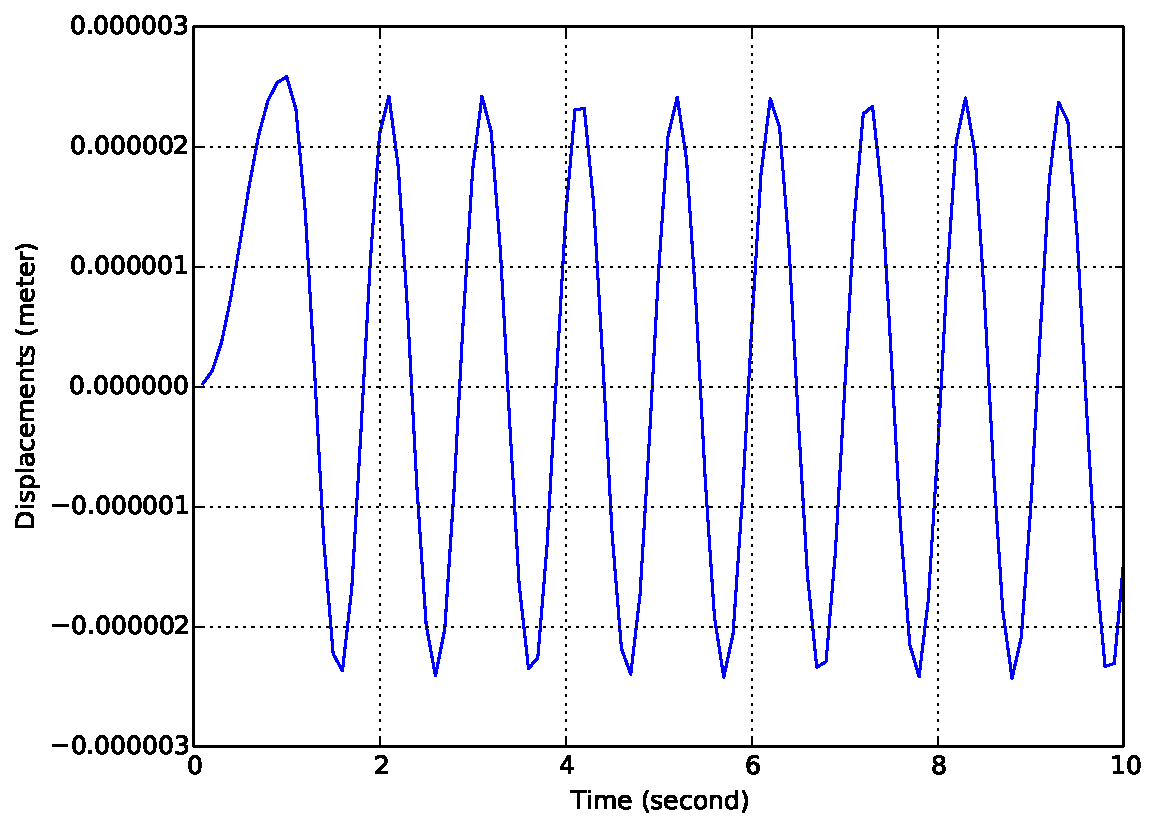
\includegraphics[width=12cm]{./Figure-files/_Chapter_Appendix_Illustrative_Examples/beam-1element-freeVibration.pdf}
  \caption{Simulate the cantilever by 1 elastic beam element under the free vibration}
  \label{fig_beam1_freevib}
\end{figure}



% The    ESSI   model   fei   files   for   this   example   can   be   downloaded
% \href{https://github.com/BorisJeremic/Real-ESSI-Examples/blob/master/model_fei_file/shearbeam_pisano_plastic8NodeBrickLT_DruckerPragerArmstrongFrederick/8NodeBrickLT_DruckerPragerArmstrongFrederick.tgz?raw=true}{here}.






















%%%%%%%%%%%%%%%%%%%%%%%%%%%%%%%%%%%%%%%%%%%%%%%%%%%%%%%%%%%%%%%%%%%%%%%%%%%%%%%%
%%%%%%%%%%%%%%%%%%%%%%%%%%%%%%%%%%%%%%%%%%%%%%%%%%%%%%%%%%%%%%%%%%%%%%%%%%%%%%%%
%%%%%%%%%%%%%%%%%%%%%%%%%%%%%%%%%%%%%%%%%%%%%%%%%%%%%%%%%%%%%%%%%%%%%%%%%%%%%%%%
%%%%%%%%%%%%%%%%%%%%%%%%%%%%%%%%%%%%%%%%%%%%%%%%%%%%%%%%%%%%%%%%%%%%%%%%%%%%%%%%
%%%%%%%%%%%%%%%%%%%%%%%%%%%%%%%%%%%%%%%%%%%%%%%%%%%%%%%%%%%%%%%%%%%%%%%%%%%%%%%%
%%%%%%%%%%%%%%%%%%%%%%%%%%%%%%%%%%%%%%%%%%%%%%%%%%%%%%%%%%%%%%%%%%%%
%%%%%%%%%%%%%%%%%%%%%%%%%%%%%%%%%%%%%%%%%%%%%%%%%%%%%%%%%%%%%%%%%%%%

\newpage
\subsection{Simulate the cantilever by 5 elastic beam element} 
\paragraph{Problem description:} ~

\begin{itemize}
  \item Structure size

    Structure Length=1m, width=0.2m, height=0.2m.

  \item Element size

    Element length=0.2m, width=0.2m, height=0.2m.
\end{itemize}

\begin{figure}[!htb]
  \centering
  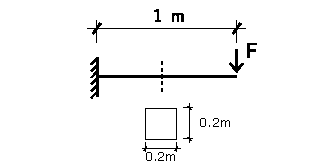
\includegraphics[width=12cm]{./Figure-files/_Chapter_Appendix_Illustrative_Examples/cantilever.pdf}
  \caption{The cantilever model}
  \label{fig_cantilever_m5}
\end{figure}


\paragraph{ESSI model fei file: } ~

\begin{lstlisting}
model name "beam_5element" ;

// add node
add node #  1 at (   0.0*m ,    0.0*m,     0.0*m)  with 6 dofs;
add node #  2 at (   0.2*m ,    0.0*m,     0.0*m)  with 6 dofs;
add node #  3 at (   0.4*m ,    0.0*m,     0.0*m)  with 6 dofs;
add node #  4 at (   0.6*m ,    0.0*m,     0.0*m)  with 6 dofs;
add node #  5 at (   0.8*m ,    0.0*m,     0.0*m)  with 6 dofs;
add node #  6 at (   1.0*m ,    0.0*m,     0.0*m)  with 6 dofs;
  
// Geometry: width and height
b=0.2*m;
h=0.2*m;

// Materials: properties
natural_period    = 1*s;        
natural_frequency  = 2*pi/natural_period;
elastic_constant  = 1e9*N/m^2; 
I=b*h^3/12.0;
A=b*h;
L=1*m;
rho   = (1.8751)^4*elastic_constant*I/(natural_frequency^2*L^4*A);
possion_ratio=0.3;

// add elements
ii=1;
while (ii<6) {
  add element # ii type beam_elastic with nodes (ii,ii+1) 
    cross_section =   b*h 
    elastic_modulus =  elastic_constant
    shear_modulus =  elastic_constant/2/(1+possion_ratio)
    torsion_Jx =  0.33*b*h^3
    bending_Iy =  b*h^3/12
    bending_Iz =  b*h^3/12
    mass_density = rho
    xz_plane_vector = ( 1, 0, 1) 
    joint_1_offset = (0*m, 0*m, 0*m) 
    joint_2_offset = (0*m, 0*m, 0*m);
  ii+=1;
}

// add boundary condition
fix node #      1 dofs all;

// // ----------------------------------------------------------------------------
// // --slowLoading---------------------------------------------------------------
// // add the 1 Newton load in 180 seconds. 
// // ----------------------------------------------------------------------------
// new loading stage "slowLoading";
// add load # 1 to node # 6 type path_time_series 
//  Fz =  1.*N
//  series_file = "slowLoading.txt" ;
// define dynamic integrator Newmark with gamma = 0.5 beta = 0.25;
// define algorithm With_no_convergence_check ;
// define solver ProfileSPD;
// simulate 2000 steps using transient algorithm 
//  time_step = 0.1*s;

// // ----------------------------------------------------------------------------
// // --fastLoading---------------------------------------------------------------
// // add the 1 Newton load in 0.6 seconds.
// // ----------------------------------------------------------------------------
// remove load # 1;
// new loading stage "fastLoading";
// add load # 2 to node # 6 type path_time_series 
//  Fz =  1.*N
//  series_file = "fastLoading.txt" ;
// define dynamic integrator Newmark with gamma = 0.5 beta = 0.25;
// define algorithm With_no_convergence_check ;
// define solver ProfileSPD;
// simulate 1000 steps using transient algorithm 
//  time_step = 0.01*s;

// // ----------------------------------------------------------------------------
// // --freeVibration-------------------------------------------------------------
// // add a load and then release to free vibration
// // ----------------------------------------------------------------------------
// remove load # 2;
new loading stage "freeVibration";
add load # 3 to node # 6 type path_time_series 
  Fz =  1.*N
  series_file = "freeVibration.txt" ;
define dynamic integrator Newmark with gamma = 0.5 beta = 0.25;
define algorithm With_no_convergence_check ;
define solver ProfileSPD;
simulate 100 steps using transient algorithm 
  time_step = 0.1*s;

bye;
\end{lstlisting}

\paragraph{Displacement results against time series} ~

\begin{figure}[!htb]
  \centering
  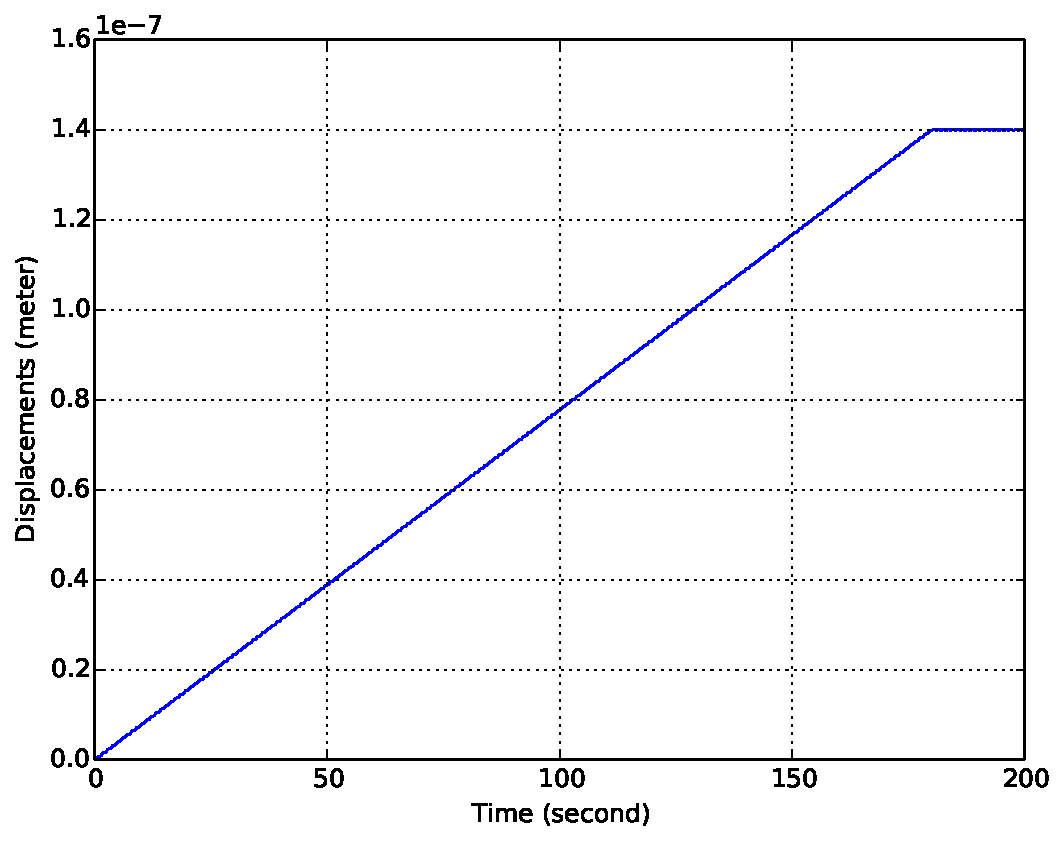
\includegraphics[width=12cm]{./Figure-files/_Chapter_Appendix_Illustrative_Examples/beam-5element-slowLoading.pdf}
  \caption{Simulate the cantilever by 1 elastic beam element under the slow loading}
  \label{fig_beam5_slow}
\end{figure}


\begin{figure}[!htb]
  \centering
  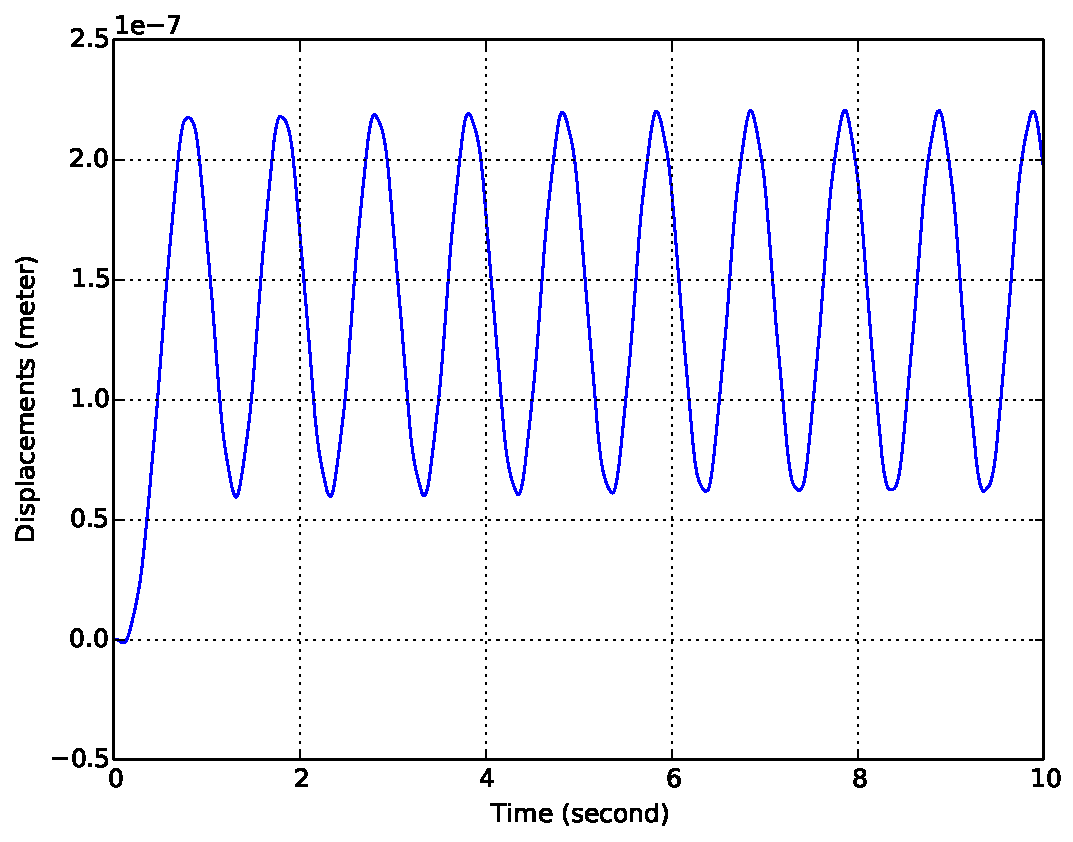
\includegraphics[width=12cm]{./Figure-files/_Chapter_Appendix_Illustrative_Examples/beam-5element-fastLoading.pdf}
  \caption{Simulate the cantilever by 1 elastic beam element under the fast loading}
  \label{fig_beam5_fast}
\end{figure}

\begin{figure}[!htb]
  \centering
  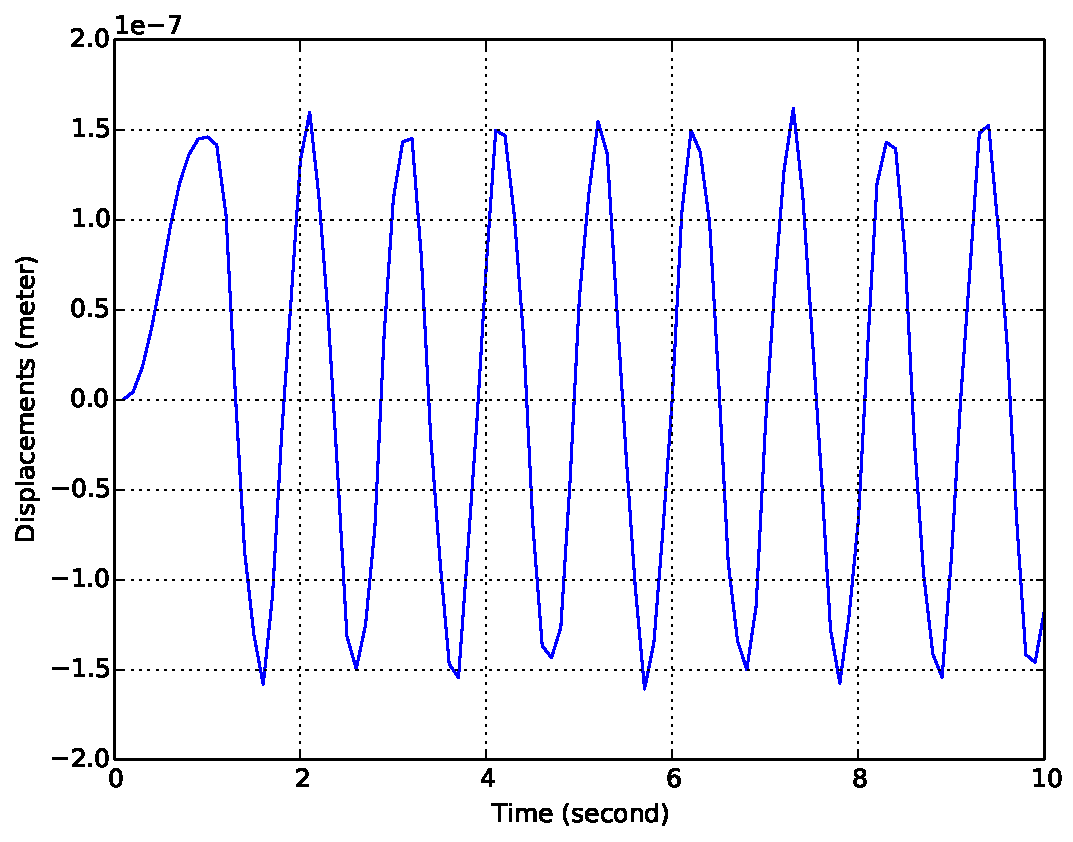
\includegraphics[width=12cm]{./Figure-files/_Chapter_Appendix_Illustrative_Examples/beam-5element-freeVibration.pdf}
  \caption{Simulate the cantilever by 1 elastic beam element under the free vibration}
  \label{fig_beam5_freevibration}
\end{figure}


























%%%%%%%%%%%%%%%%%%%%%%%%%%%%%%%%%%%%%%%%%%%%%%%%%%%%%%%%%%%%%%%%%%%%%%%%%%%%%%%%
%%%%%%%%%%%%%%%%%%%%%%%%%%%%%%%%%%%%%%%%%%%%%%%%%%%%%%%%%%%%%%%%%%%%%%%%%%%%%%%%
%%%%%%%%%%%%%%%%%%%%%%%%%%%%%%%%%%%%%%%%%%%%%%%%%%%%%%%%%%%%%%%%%%%%%%%%%%%%%%%%
%%%%%%%%%%%%%%%%%%%%%%%%%%%%%%%%%%%%%%%%%%%%%%%%%%%%%%%%%%%%%%%%%%%%%%%%%%%%%%%%
%%%%%%%%%%%%%%%%%%%%%%%%%%%%%%%%%%%%%%%%%%%%%%%%%%%%%%%%%%%%%%%%%%%%%%%%%%%%%%%%
%%%%%%%%%%%%%%%%%%%%%%%%%%%%%%%%%%%%%%%%%%%%%%%%%%%%%%%%%%%%%%%%%%%%
%%%%%%%%%%%%%%%%%%%%%%%%%%%%%%%%%%%%%%%%%%%%%%%%%%%%%%%%%%%%%%%%%%%%

\newpage
\section{27NodeBrick Element under Dynamic Loading} ~ 
\subsection{Simulate the cantilever by one 27NodeBrick element} 
\paragraph{Problem description:} ~

\begin{itemize}
  \item Structure size

    Structure Length=1m, width=0.2m, height=0.2m.

  \item Element size

    Element length=1m, width=0.2m, height=0.2m.
\end{itemize}

\begin{figure}[!htb]
  \centering
  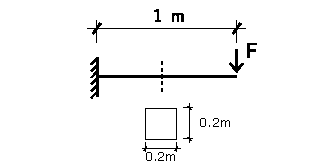
\includegraphics[width=12cm]{./Figure-files/_Chapter_Appendix_Illustrative_Examples/cantilever.pdf}
  \caption{The cantilever model}
  \label{fig_cantilev_1}
\end{figure}


\paragraph{ESSI model fei file: } ~

\begin{lstlisting}
model name "brick_1element" ;

// Geometry: width and height
b=0.2*m;
h=0.2*m;

// Materials: properties
natural_period    = 1*s;        
natural_frequency  = 2*pi/natural_period;
elastic_constant  = 1e9*N/m^2; 
I=b*h^3/12.0;
A=b*h;
L=1*m;
rho   = (1.8751)^4*elastic_constant*I/(natural_frequency^2*L^4*A);
possion_ratio=0.3;


add material # 1 type linear_elastic_isotropic_3d_LT
  mass_density = rho
  elastic_modulus = elastic_constant
  poisson_ratio = possion_ratio;

add node #        1 at (   0.0000 *m,   0.2000 *m,  0.0000 *m) with 3 dofs;
add node #        2 at (   0.0000 *m,   0.0000 *m,  0.0000 *m) with 3 dofs;
add node #        3 at (   1.0000 *m,   0.2000 *m,  0.0000 *m) with 3 dofs;
add node #        4 at (   1.0000 *m,   0.0000 *m,  0.0000 *m) with 3 dofs;
add node #        5 at (   0.0000 *m,   0.0000 *m,  0.2000 *m) with 3 dofs;
add node #        6 at (   1.0000 *m,   0.0000 *m,  0.2000 *m) with 3 dofs;
add node #        7 at (   1.0000 *m,   0.2000 *m,  0.2000 *m) with 3 dofs;
add node #        8 at (   0.0000 *m,   0.2000 *m,  0.2000 *m) with 3 dofs;
add node #        9 at (   0.0000 *m,   0.1000 *m,  0.0000 *m) with 3 dofs;
add node #       10 at (   0.5000 *m,   0.2000 *m,  0.0000 *m) with 3 dofs;
add node #       11 at (   1.0000 *m,   0.1000 *m,  0.0000 *m) with 3 dofs;
add node #       12 at (   0.5000 *m,   0.0000 *m,  0.0000 *m) with 3 dofs;
add node #       13 at (   0.0000 *m,   0.1000 *m,  0.2000 *m) with 3 dofs;
add node #       14 at (   0.5000 *m,   0.2000 *m,  0.2000 *m) with 3 dofs;
add node #       15 at (   1.0000 *m,   0.1000 *m,  0.2000 *m) with 3 dofs;
add node #       16 at (   0.5000 *m,   0.0000 *m,  0.2000 *m) with 3 dofs;
add node #       17 at (   0.0000 *m,   0.0000 *m,  0.1000 *m) with 3 dofs;
add node #       18 at (   0.0000 *m,   0.2000 *m,  0.1000 *m) with 3 dofs;
add node #       19 at (   1.0000 *m,   0.2000 *m,  0.1000 *m) with 3 dofs;
add node #       20 at (   1.0000 *m,   0.0000 *m,  0.1000 *m) with 3 dofs;
add node #       21 at (   0.5000 *m,   0.1000 *m,  0.1000 *m) with 3 dofs;
add node #       22 at (   0.0000 *m,   0.1000 *m,  0.1000 *m) with 3 dofs;
add node #       23 at (   0.5000 *m,   0.2000 *m,  0.1000 *m) with 3 dofs;
add node #       24 at (   1.0000 *m,   0.1000 *m,  0.1000 *m) with 3 dofs;
add node #       25 at (   0.5000 *m,   0.0000 *m,  0.1000 *m) with 3 dofs;
add node #       26 at (   0.5000 *m,   0.1000 *m,  0.0000 *m) with 3 dofs;
add node #       27 at (   0.5000 *m,   0.1000 *m,  0.2000 *m) with 3 dofs;

add element #         1 type 27NodeBrickLT with nodes(       2,       1,       3,       4,       5,       8,       7,       6,       9,      10,      11,      12,      13,      14,      15,      16,      17,      18,      19,      20,      21,      22,      23,      24,      25,      26,      27) use material #        1; 

fix node # 1 dofs all;
fix node # 2 dofs all;
fix node # 5 dofs all;
fix node # 8 dofs all;
fix node # 9 dofs all;
fix node # 13 dofs all;
fix node # 17 dofs all;
fix node # 18 dofs all;
fix node # 22 dofs all;

  
// // ----------------------------------------------------------------------------
// // --slowLoading---------------------------------------------------------------
// // ----------------------------------------------------------------------------
// new loading stage "slowLoading";
// add load # 1 to node # 4 type path_time_series Fz=1/36.0*N series_file = "slowLoading.txt" ; 
// add load # 2 to node # 6 type path_time_series Fz=1/36.0*N series_file = "slowLoading.txt" ; 
// add load # 3 to node # 3 type path_time_series Fz=1/36.0*N series_file = "slowLoading.txt" ; 
// add load # 4 to node # 7 type path_time_series Fz=1/36.0*N series_file = "slowLoading.txt" ; 
// add load # 5 to node # 20 type path_time_series Fz=1/9.0*N series_file = "slowLoading.txt" ; 
// add load # 6 to node # 11 type path_time_series Fz=1/9.0*N series_file = "slowLoading.txt" ; 
// add load # 7 to node # 15 type path_time_series Fz=1/9.0*N series_file = "slowLoading.txt" ; 
// add load # 8 to node # 19 type path_time_series Fz=1/9.0*N series_file = "slowLoading.txt" ; 
// add load # 9 to node # 24 type path_time_series Fz=4/9.0*N series_file = "slowLoading.txt" ; 
// // add algorithm and solver
// define dynamic integrator Newmark with gamma = 0.5 beta = 0.25;
// define algorithm With_no_convergence_check ;
// define solver ProfileSPD;
// simulate 2000 steps using transient algorithm 
//  time_step = 0.1*s;

// // ----------------------------------------------------------------------------
// // --fastLoading---------------------------------------------------------------
// // ----------------------------------------------------------------------------
// new loading stage "fastLoading";
// add load # 101 to node # 4 type path_time_series Fz=1/36.0*N series_file = "fastLoading.txt" ; 
// add load # 102 to node # 6 type path_time_series Fz=1/36.0*N series_file = "fastLoading.txt" ; 
// add load # 103 to node # 3 type path_time_series Fz=1/36.0*N series_file = "fastLoading.txt" ; 
// add load # 104 to node # 7 type path_time_series Fz=1/36.0*N series_file = "fastLoading.txt" ; 
// add load # 105 to node # 20 type path_time_series Fz=1/9.0*N series_file = "fastLoading.txt" ; 
// add load # 106 to node # 11 type path_time_series Fz=1/9.0*N series_file = "fastLoading.txt" ; 
// add load # 107 to node # 15 type path_time_series Fz=1/9.0*N series_file = "fastLoading.txt" ; 
// add load # 108 to node # 19 type path_time_series Fz=1/9.0*N series_file = "fastLoading.txt" ; 
// add load # 109 to node # 24 type path_time_series Fz=4/9.0*N series_file = "fastLoading.txt" ; 
// // add algorithm and solver
// define dynamic integrator Newmark with gamma = 0.5 beta = 0.25;
// define algorithm With_no_convergence_check ;
// define solver ProfileSPD;
// simulate 1000 steps using transient algorithm 
//  time_step = 0.01*s;

// // ----------------------------------------------------------------------------
// // --freeVibration---------------------------------------------------------------
// // ----------------------------------------------------------------------------
new loading stage "freeVibration";
add load # 201 to node # 4 type path_time_series Fz=1/36.0*N series_file = "freeVibration.txt" ; 
add load # 202 to node # 6 type path_time_series Fz=1/36.0*N series_file = "freeVibration.txt" ; 
add load # 203 to node # 3 type path_time_series Fz=1/36.0*N series_file = "freeVibration.txt" ; 
add load # 204 to node # 7 type path_time_series Fz=1/36.0*N series_file = "freeVibration.txt" ; 
add load # 205 to node # 20 type path_time_series Fz=1/9.0*N series_file = "freeVibration.txt" ; 
add load # 206 to node # 11 type path_time_series Fz=1/9.0*N series_file = "freeVibration.txt" ; 
add load # 207 to node # 15 type path_time_series Fz=1/9.0*N series_file = "freeVibration.txt" ; 
add load # 208 to node # 19 type path_time_series Fz=1/9.0*N series_file = "freeVibration.txt" ; 
add load # 209 to node # 24 type path_time_series Fz=4/9.0*N series_file = "freeVibration.txt" ; 
// add algorithm and solver
define dynamic integrator Newmark with gamma = 0.5 beta = 0.25;
define algorithm With_no_convergence_check ;
define solver ProfileSPD;
simulate 10000 steps using transient algorithm 
  time_step = 0.001*s;

// end
bye;
\end{lstlisting}

\paragraph{Displacement results against time series} ~

\begin{figure}[!htb]
  \centering
  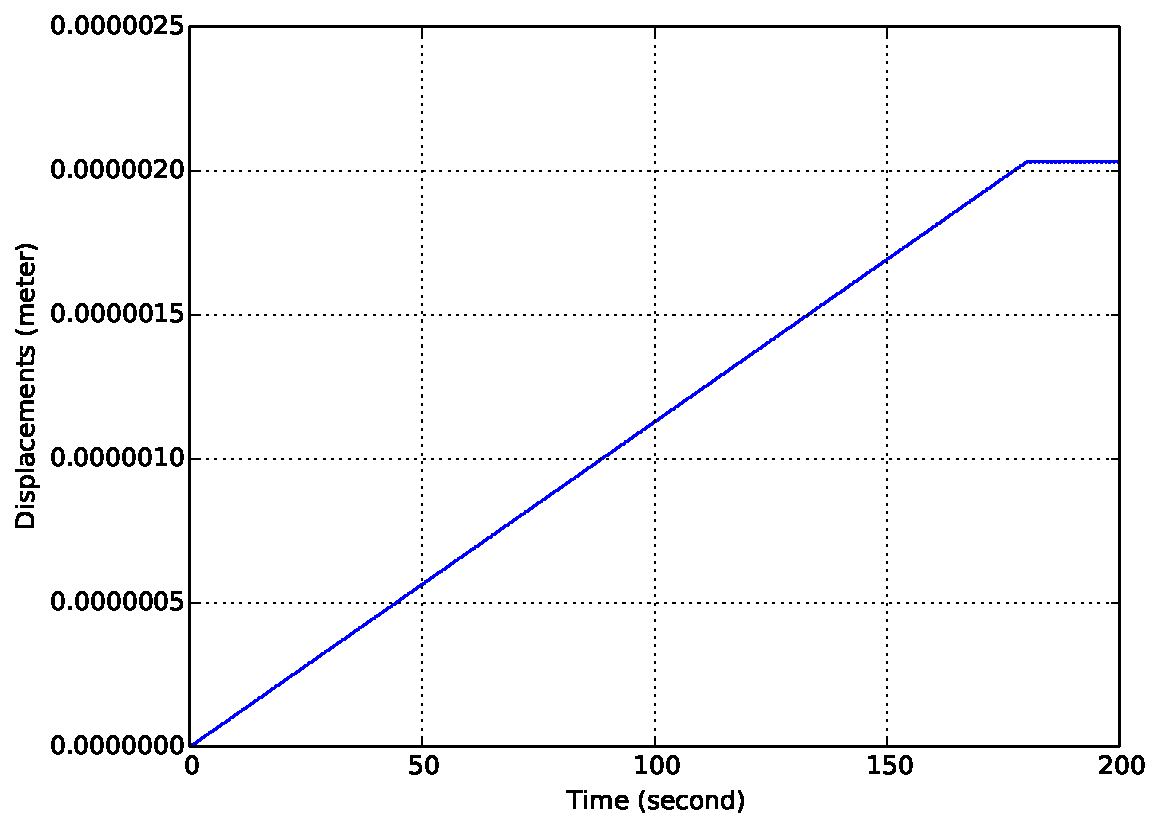
\includegraphics[width=12cm]{./Figure-files/_Chapter_Appendix_Illustrative_Examples/brick-1element-slowLoading.pdf}
  \caption{Simulate the cantilever by one 27NodeBrick element under the slow loading}
  \label{fig_brick1-slow}
\end{figure}


\begin{figure}[!htb]
  \centering
  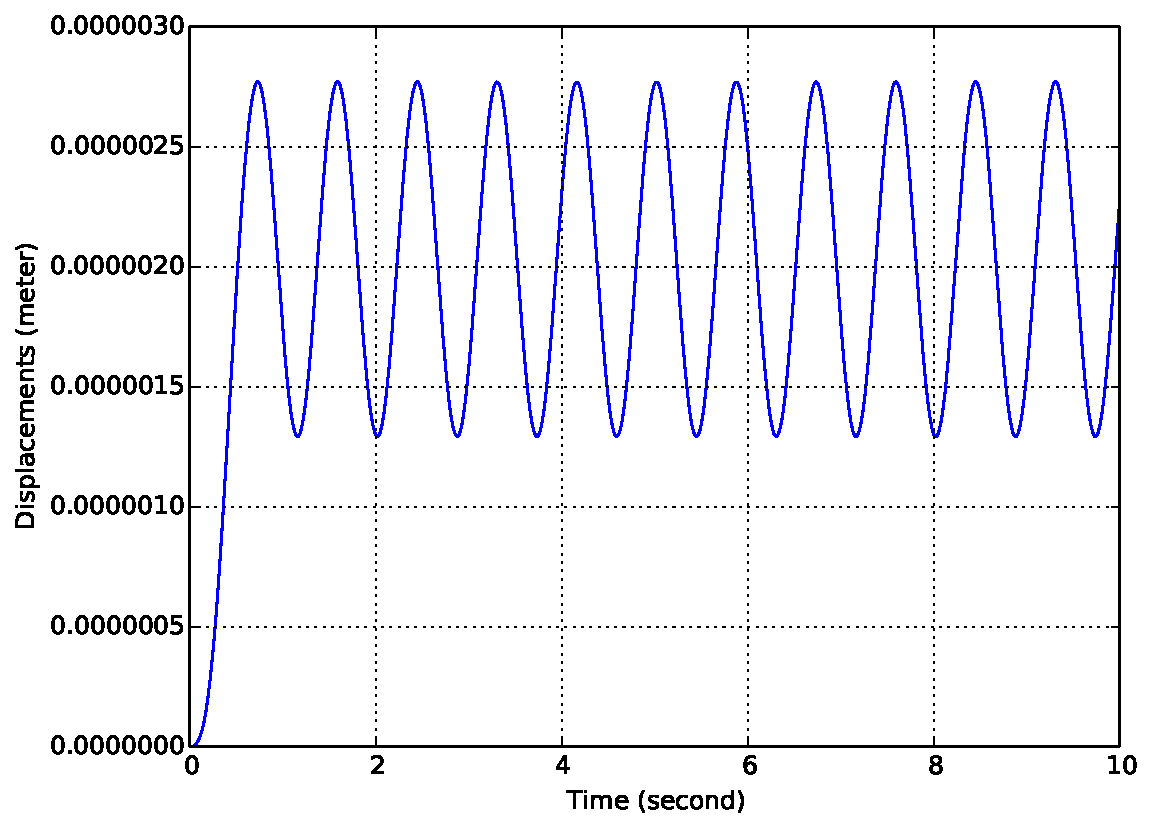
\includegraphics[width=12cm]{./Figure-files/_Chapter_Appendix_Illustrative_Examples/brick-1element-fastLoading.pdf}
  \caption{Simulate the cantilever by one 27NodeBrick element under the fast loading}
  \label{fig_brick1-fast}
\end{figure}

\begin{figure}[!htb]
  \centering
  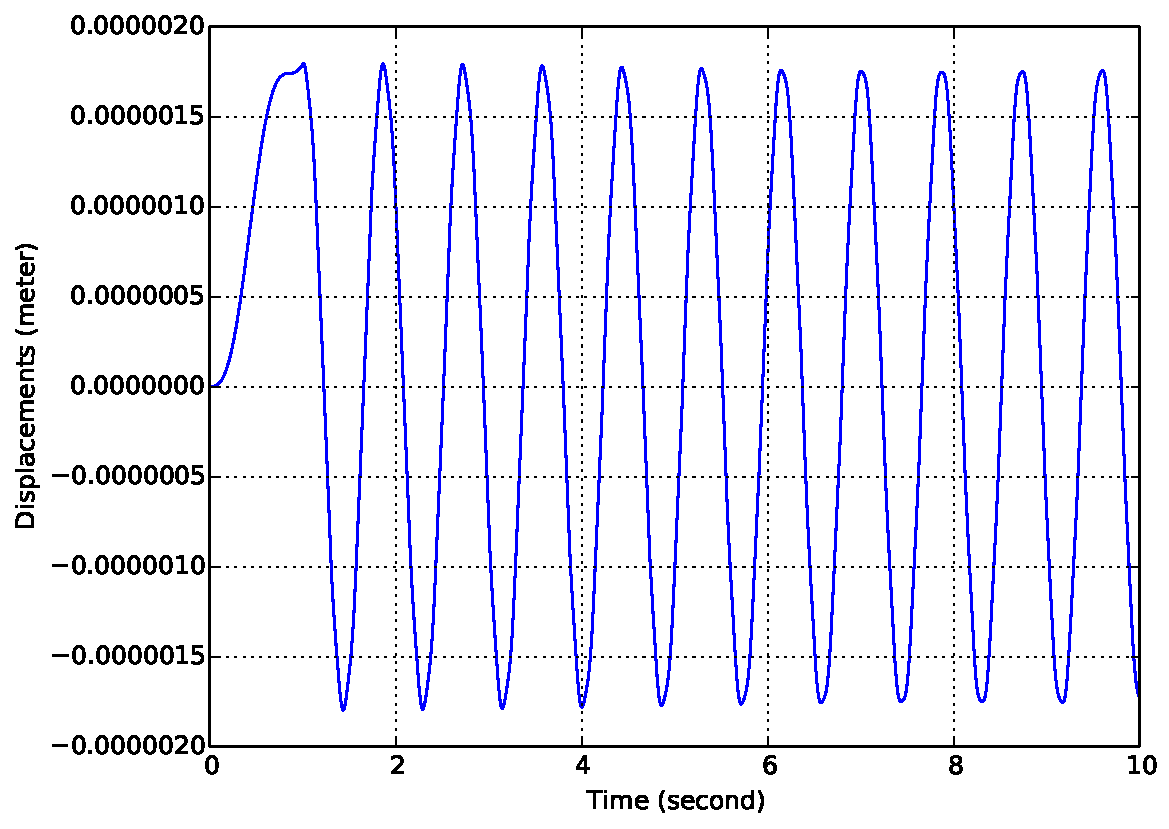
\includegraphics[width=12cm]{./Figure-files/_Chapter_Appendix_Illustrative_Examples/brick-1element-freeVibration.pdf}
  \caption{Simulate the cantilever by one 27NodeBrick element under the free vibration}
  \label{fig_brick1-freevib}
\end{figure}



% The    ESSI   model   fei   files   for   this   example   can   be   downloaded
% \href{https://github.com/BorisJeremic/Real-ESSI-Examples/blob/master/model_fei_file/shearbeam_pisano_plastic8NodeBrickLT_DruckerPragerArmstrongFrederick/8NodeBrickLT_DruckerPragerArmstrongFrederick.tgz?raw=true}{here}.









%%%%%%%%%%%%%%%%%%%%%%%%%%%%%%%%%%%%%%%%%%%%%%%%%%%%%%%%%%%%%%%%%%%%%%%%%%%%%%%%
%%%%%%%%%%%%%%%%%%%%%%%%%%%%%%%%%%%%%%%%%%%%%%%%%%%%%%%%%%%%%%%%%%%%%%%%%%%%%%%%
%%%%%%%%%%%%%%%%%%%%%%%%%%%%%%%%%%%%%%%%%%%%%%%%%%%%%%%%%%%%%%%%%%%%%%%%%%%%%%%%
%%%%%%%%%%%%%%%%%%%%%%%%%%%%%%%%%%%%%%%%%%%%%%%%%%%%%%%%%%%%%%%%%%%%%%%%%%%%%%%%
%%%%%%%%%%%%%%%%%%%%%%%%%%%%%%%%%%%%%%%%%%%%%%%%%%%%%%%%%%%%%%%%%%%%%%%%%%%%%%%%
%%%%%%%%%%%%%%%%%%%%%%%%%%%%%%%%%%%%%%%%%%%%%%%%%%%%%%%%%%%%%%%%%%%%
%%%%%%%%%%%%%%%%%%%%%%%%%%%%%%%%%%%%%%%%%%%%%%%%%%%%%%%%%%%%%%%%%%%%

\newpage
\subsection{Simulate the cantilever by five 27NodeBrick element} 
\paragraph{Problem description:} ~

\begin{itemize}
  \item Structure size

    Structure Length=1m, width=0.2m, height=0.2m.

  \item Element size

    Element length=0.2m, width=0.2m, height=0.2m.
\end{itemize}

\begin{figure}[!htb]
  \centering
  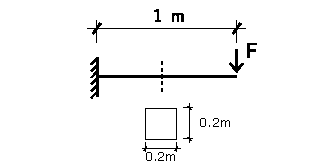
\includegraphics[width=12cm]{./Figure-files/_Chapter_Appendix_Illustrative_Examples/cantilever.pdf}
  \caption{The cantilever model}
  % \label{}
\end{figure}


\paragraph{ESSI model fei file: } ~

\begin{lstlisting}
model name "brick_5element" ;

// Geometry: width and height
b=0.2*m;
h=0.2*m;

// Materials: properties
natural_period    = 1*s;        
natural_frequency  = 2*pi/natural_period;
elastic_constant  = 1e9*N/m^2; 
I=b*h^3/12.0;
A=b*h;
L=1*m;
rho   = (1.8751)^4*elastic_constant*I/(natural_frequency^2*L^4*A);
possion_ratio=0.3;


add material # 1 type linear_elastic_isotropic_3d_LT
  mass_density = rho
  elastic_modulus = elastic_constant
  poisson_ratio = possion_ratio;

add node # 1 at (0.0*m, 0.0*m , 0.0*m) with 3 dofs;
add node # 2 at (0.1*m, 0.0*m , 0.0*m) with 3 dofs;
add node # 3 at (0.2*m, 0.0*m , 0.0*m) with 3 dofs;
add node # 4 at (0.0*m, 0.1*m , 0.0*m) with 3 dofs;
add node # 5 at (0.1*m, 0.1*m , 0.0*m) with 3 dofs;
add node # 6 at (0.2*m, 0.1*m , 0.0*m) with 3 dofs;
add node # 7 at (0.0*m, 0.2*m , 0.0*m) with 3 dofs;
add node # 8 at (0.1*m, 0.2*m , 0.0*m) with 3 dofs;
add node # 9 at (0.2*m, 0.2*m , 0.0*m) with 3 dofs;

fix node No 1 dofs ux uy uz;
fix node No 2 dofs ux uy uz;
fix node No 3 dofs ux uy uz;
fix node No 4 dofs ux uy uz;
fix node No 5 dofs ux uy uz;
fix node No 6 dofs ux uy uz;
fix node No 7 dofs ux uy uz;
fix node No 8 dofs ux uy uz;
fix node No 9 dofs ux uy uz;
e = 0;
hh = 0*m;
NBricks=5;
dz = 0.2*m;
while ( e < NBricks)
{
  hh += dz;
  add node # 10+18*e at (0.0*m, 0.0*m , hh - 0.5*dz) with 3 dofs;
  add node # 11+18*e at (0.1*m, 0.0*m , hh - 0.5*dz) with 3 dofs;
  add node # 12+18*e at (0.2*m, 0.0*m , hh - 0.5*dz) with 3 dofs;
  add node # 13+18*e at (0.0*m, 0.1*m , hh - 0.5*dz) with 3 dofs;
  add node # 14+18*e at (0.1*m, 0.1*m , hh - 0.5*dz) with 3 dofs;
  add node # 15+18*e at (0.2*m, 0.1*m , hh - 0.5*dz) with 3 dofs;
  add node # 16+18*e at (0.0*m, 0.2*m , hh - 0.5*dz) with 3 dofs;
  add node # 17+18*e at (0.1*m, 0.2*m , hh - 0.5*dz) with 3 dofs;
  add node # 18+18*e at (0.2*m, 0.2*m , hh - 0.5*dz) with 3 dofs;
  
  add node # 19+18*e at (0.0*m, 0.0*m , hh) with 3 dofs;
  add node # 20+18*e at (0.1*m, 0.0*m , hh) with 3 dofs;
  add node # 21+18*e at (0.2*m, 0.0*m , hh) with 3 dofs;
  add node # 22+18*e at (0.0*m, 0.1*m , hh) with 3 dofs;
  add node # 23+18*e at (0.1*m, 0.1*m , hh) with 3 dofs;
  add node # 24+18*e at (0.2*m, 0.1*m , hh) with 3 dofs;
  add node # 25+18*e at (0.0*m, 0.2*m , hh) with 3 dofs;
  add node # 26+18*e at (0.1*m, 0.2*m , hh) with 3 dofs;
  add node # 27+18*e at (0.2*m, 0.2*m , hh) with 3 dofs;

  add element # e+1 type 27NodeBrickLT with nodes 
    (
      21+18*e,
      27+18*e,
      25+18*e,
      19+18*e,

       3+18*e,
       9+18*e,
       7+18*e,
       1+18*e,

      24+18*e,
      26+18*e,
      22+18*e,
      20+18*e,

       6+18*e,
       8+18*e,
       4+18*e,
       2+18*e,

      12+18*e,
      18+18*e,
      16+18*e,
      10+18*e,

      14+18*e,
      15+18*e,
      17+18*e,
      13+18*e,
      11+18*e,
      23+18*e,
       5+18*e
    ) 
    use material # 1;

  e += 1;
};


e = e -1;

  
// // ----------------------------------------------------------------------------
// // --slowLoading---------------------------------------------------------------
// // add the 1 Newton load in 180 seconds. 
// // ----------------------------------------------------------------------------
// new loading stage "slowLoading";
// add load # 1 to node # (19+18*e) type path_time_series Fx=1/36.0*N series_file = "slowLoading.txt";
// add load # 2 to node # (20+18*e) type path_time_series Fx=1/9.0*N series_file = "slowLoading.txt";
// add load # 3 to node # (21+18*e) type path_time_series Fx=1/36.0*N series_file = "slowLoading.txt";
// add load # 4 to node # (22+18*e) type path_time_series Fx=1/9.0*N series_file = "slowLoading.txt";
// add load # 5 to node # (23+18*e) type path_time_series Fx=4/9.0*N series_file = "slowLoading.txt";
// add load # 6 to node # (24+18*e) type path_time_series Fx=1/9.0*N series_file = "slowLoading.txt";
// add load # 7 to node # (25+18*e) type path_time_series Fx=1/36.0*N series_file = "slowLoading.txt";
// add load # 8 to node # (26+18*e) type path_time_series Fx=1/9.0*N series_file = "slowLoading.txt";
// add load # 9 to node # (27+18*e) type path_time_series Fx=1/36.0*N series_file = "slowLoading.txt";
// // add algorithm and solver
// define dynamic integrator Newmark with gamma = 0.5 beta = 0.25;
// define algorithm With_no_convergence_check ;
// define solver ProfileSPD;
// simulate 2000 steps using transient algorithm 
//  time_step = 0.1*s;

// // ----------------------------------------------------------------------------
// // --fastLoading---------------------------------------------------------------
// // add the 1 Newton load in 0.6 seconds.
// // ----------------------------------------------------------------------------
// new loading stage "fastLoading";
// add load # 101 to node # (19+18*e) type path_time_series Fx=1/36.0*N series_file = "fastLoading.txt" ; 
// add load # 102 to node # (20+18*e) type path_time_series Fx=1/9.0*N series_file = "fastLoading.txt" ; 
// add load # 103 to node # (21+18*e) type path_time_series Fx=1/36.0*N series_file = "fastLoading.txt" ; 
// add load # 104 to node # (22+18*e) type path_time_series Fx=1/9.0*N series_file = "fastLoading.txt" ; 
// add load # 105 to node # (23+18*e) type path_time_series Fx=4/9.0*N series_file = "fastLoading.txt" ; 
// add load # 106 to node # (24+18*e) type path_time_series Fx=1/9.0*N series_file = "fastLoading.txt" ; 
// add load # 107 to node # (25+18*e) type path_time_series Fx=1/36.0*N series_file = "fastLoading.txt" ; 
// add load # 108 to node # (26+18*e) type path_time_series Fx=1/9.0*N series_file = "fastLoading.txt" ; 
// add load # 109 to node # (27+18*e) type path_time_series Fx=1/36.0*N series_file = "fastLoading.txt" ; 
// // add algorithm and solver
// define dynamic integrator Newmark with gamma = 0.5 beta = 0.25;
// define algorithm With_no_convergence_check ;
// define solver ProfileSPD;
// simulate 1000 steps using transient algorithm 
//  time_step = 0.01*s;

// // ----------------------------------------------------------------------------
// // --freeVibration---------------------------------------------------------------
// // add a load and then release to free vibration
// // ----------------------------------------------------------------------------
new loading stage "freeVibration";
add load # 201 to node # (19+18*e) type path_time_series Fx=1/36.0*N series_file = "freeVibration.txt" ; 
add load # 202 to node # (20+18*e) type path_time_series Fx=1/9.0*N series_file = "freeVibration.txt" ; 
add load # 203 to node # (21+18*e) type path_time_series Fx=1/36.0*N series_file = "freeVibration.txt" ; 
add load # 204 to node # (22+18*e) type path_time_series Fx=1/9.0*N series_file = "freeVibration.txt" ; 
add load # 205 to node # (23+18*e) type path_time_series Fx=4/9.0*N series_file = "freeVibration.txt" ; 
add load # 206 to node # (24+18*e) type path_time_series Fx=1/9.0*N series_file = "freeVibration.txt" ; 
add load # 207 to node # (25+18*e) type path_time_series Fx=1/36.0*N series_file = "freeVibration.txt" ; 
add load # 208 to node # (26+18*e) type path_time_series Fx=1/9.0*N series_file = "freeVibration.txt" ; 
add load # 209 to node # (27+18*e) type path_time_series Fx=1/36.0*N series_file = "freeVibration.txt" ; 
// add algorithm and solver
define dynamic integrator Newmark with gamma = 0.5 beta = 0.25;
define algorithm With_no_convergence_check ;
define solver ProfileSPD;
simulate 100 steps using transient algorithm 
  time_step = 0.1*s;

// end
bye;
\end{lstlisting}

\paragraph{Displacement results against time series} ~

\begin{figure}[!htb]
  \centering
  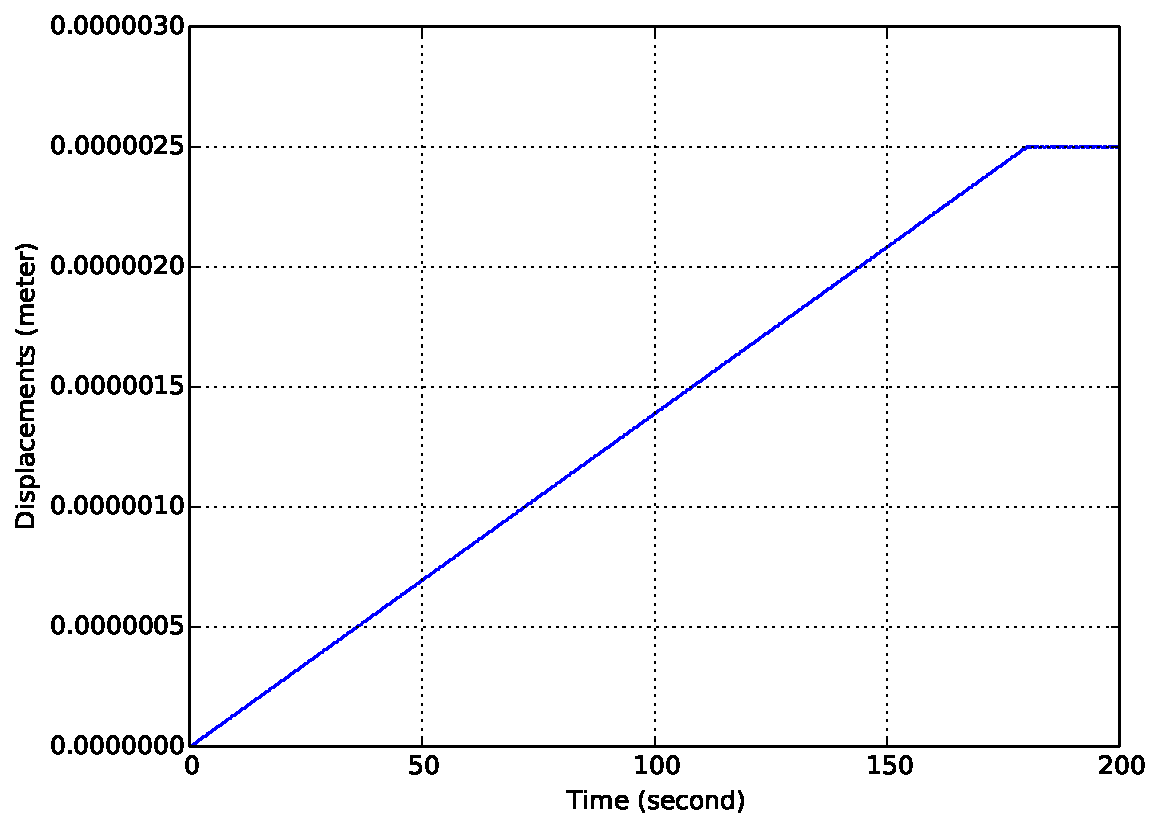
\includegraphics[width=12cm]{./Figure-files/_Chapter_Appendix_Illustrative_Examples/brick-5element-slowLoading.pdf}
  \caption{Simulate the cantilever by five 27NodeBrick elements under the slow loading}
  \label{fig_brick5-slow}
\end{figure}


\begin{figure}[!htb]
  \centering
  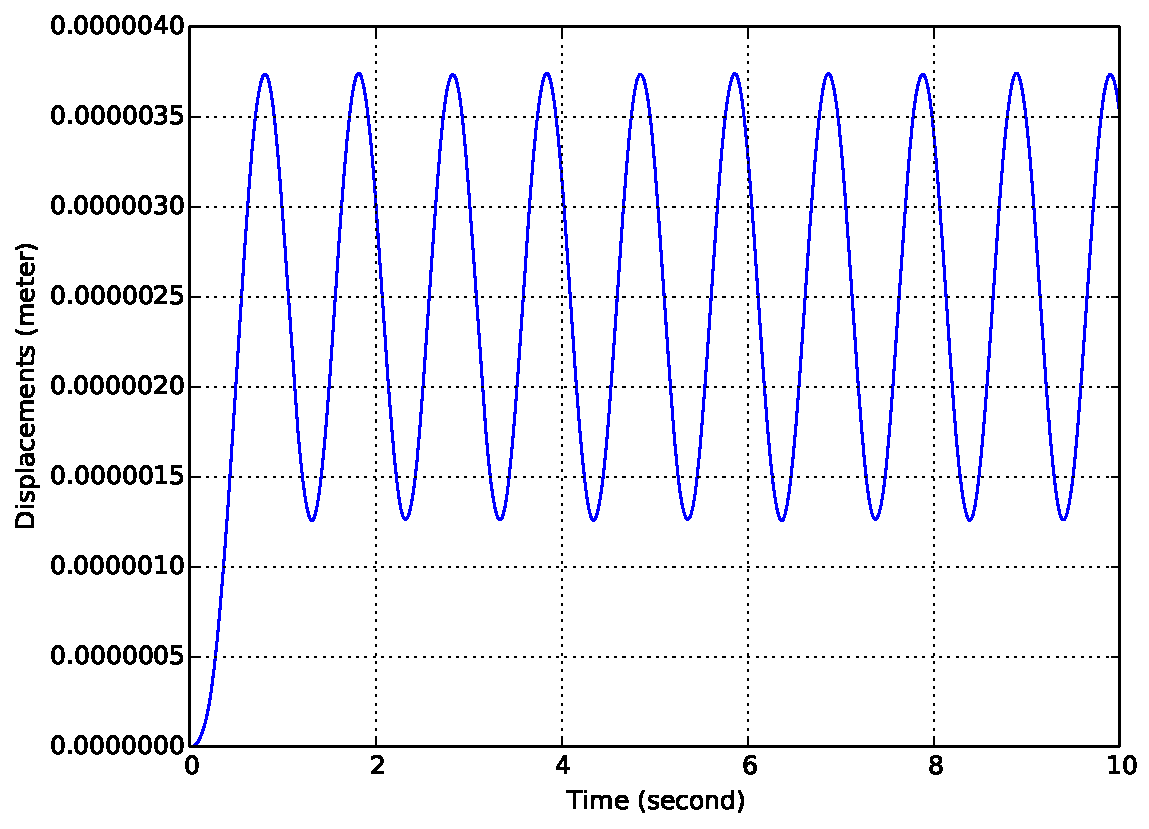
\includegraphics[width=12cm]{./Figure-files/_Chapter_Appendix_Illustrative_Examples/brick-5element-fastLoading.pdf}
  \caption{Simulate the cantilever by five 27NodeBrick elements under the fast loading}
  \label{fig_brick5-fast}
\end{figure}

\begin{figure}[!htb]
  \centering
  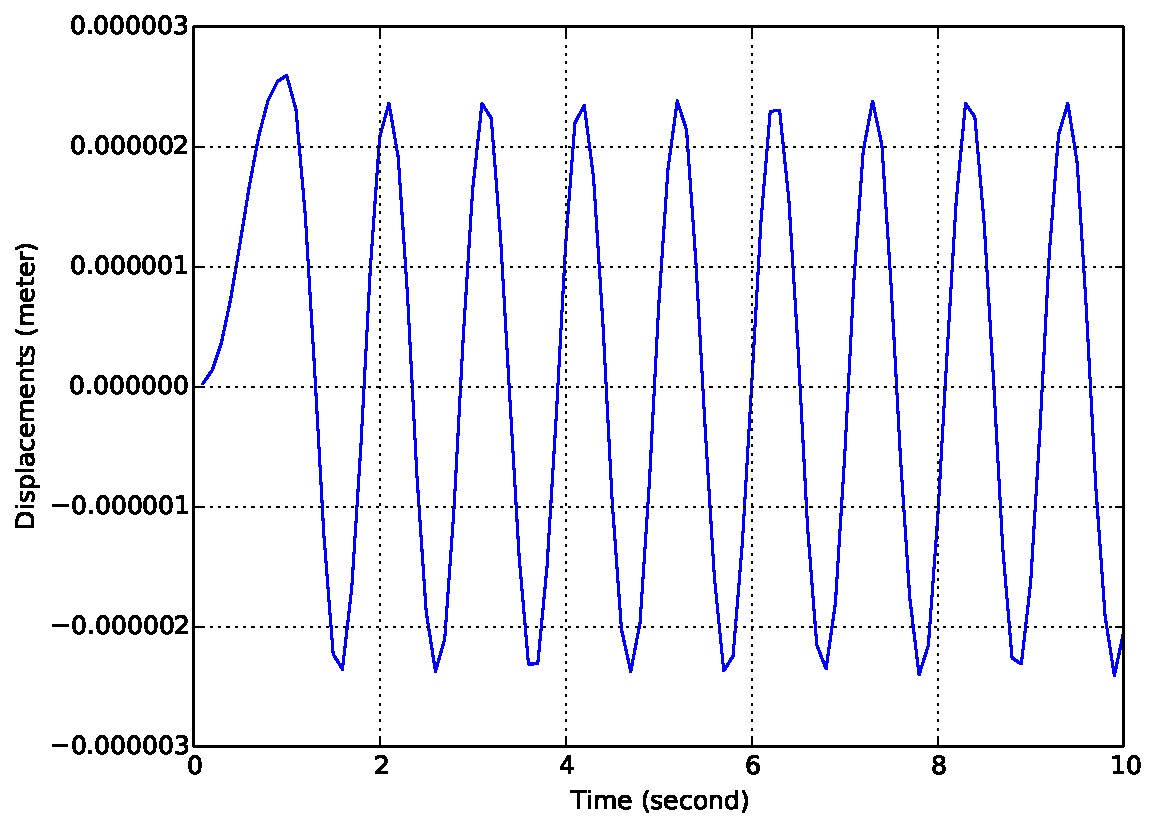
\includegraphics[width=12cm]{./Figure-files/_Chapter_Appendix_Illustrative_Examples/brick-5element-freeVibration.pdf}
  \caption{Simulate the cantilever by five 27NodeBrick elements under the free vibration}
  \label{fig_brick5-freevib}
\end{figure}





















%%%%%%%%%%%%%%%%%%%%%%%%%%%%%%%%%%%%%%%%%%%%%%%%%%%%%%%%%%%%%%%%%%%%%%%%%%%%%%%%
%%%%%%%%%%%%%%%%%%%%%%%%%%%%%%%%%%%%%%%%%%%%%%%%%%%%%%%%%%%%%%%%%%%%%%%%%%%%%%%%
%%%%%%%%%%%%%%%%%%%%%%%%%%%%%%%%%%%%%%%%%%%%%%%%%%%%%%%%%%%%%%%%%%%%%%%%%%%%%%%%
%%%%%%%%%%%%%%%%%%%%%%%%%%%%%%%%%%%%%%%%%%%%%%%%%%%%%%%%%%%%%%%%%%%%%%%%%%%%%%%%
%%%%%%%%%%%%%%%%%%%%%%%%%%%%%%%%%%%%%%%%%%%%%%%%%%%%%%%%%%%%%%%%%%%%%%%%%%%%%%%%
%%%%%%%%%%%%%%%%%%%%%%%%%%%%%%%%%%%%%%%%%%%%%%%%%%%%%%%%%%%%%%%%%%%%
%%%%%%%%%%%%%%%%%%%%%%%%%%%%%%%%%%%%%%%%%%%%%%%%%%%%%%%%%%%%%%%%%%%%

\newpage
\section{Elastic Beam Element under Dynamic Loading with concentrated mass} ~ 
\subsection{Simulate the cantilever by 1 elastic beam element} 
\paragraph{Problem description:} ~

\begin{itemize}
  \item Structure size

    Structure Length=1m, width=0.2m, height=0.2m.

  \item Element size

    Element length=1m, width=0.2m, height=0.2m.
\end{itemize}

\begin{figure}[!htb]
  \centering
  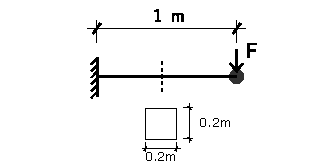
\includegraphics[width=12cm]{./Figure-files/_Chapter_Appendix_Illustrative_Examples/cantilever-mass.pdf}
  \caption{The cantilever-mass model}
  \label{fig_cantilever_mass_1}
\end{figure}


\paragraph{ESSI model fei file: } ~

\begin{lstlisting}
model name "beam-mass_1element" ;

// add node
add node #  1 at (   0.0*m ,    0.0*m,     0.0*m)  with 6 dofs;
add node #  2 at (   1.0*m ,    0.0*m,     0.0*m)  with 6 dofs;
  
// Geometry: width and height
b=0.2*m;
h=0.2*m;

// Materials: properties
natural_period    = 1*s;        
natural_frequency  = 2*pi/natural_period;
elastic_constant  = 1e9*N/m^2; 
I=b*h^3/12.0;
A=b*h;
L=1*m;
rho   = (1.8751)^4*elastic_constant*I/(natural_frequency^2*L^4*A);
possion_ratio=0.3;

// add elements
add element # 1 type beam_elastic with nodes (1,2) 
  cross_section =   b*h 
  elastic_modulus =  elastic_constant
  shear_modulus =  elastic_constant/2/(1+possion_ratio)
  torsion_Jx =  0.33*b*h^3
  bending_Iy =  b*h^3/12
  bending_Iz =  b*h^3/12
  mass_density = rho
  xz_plane_vector = ( 1, 0, 1) 
  joint_1_offset = (0*m, 0*m, 0*m) 
  joint_2_offset = (0*m, 0*m, 0*m);

// add boundary condition
fix node #      1 dofs all;

// add mass
beamMass=rho*A*L;
add mass to node # 2 
  mx = beamMass
  my = beamMass
  mz = beamMass
  Imx = 0*beamMass*L^2
  Imy = 0*beamMass*L^2
  Imz = 0*beamMass*L^2;

// // ----------------------------------------------------------------------------
// // --slowLoading---------------------------------------------------------------
// // ----------------------------------------------------------------------------
// new loading stage "slowLoading";
// add load # 1 to node # 2 type path_time_series 
//  Fz =  1.*N
//  series_file = "slowLoading.txt" ;
// define dynamic integrator Newmark with gamma = 0.5 beta = 0.25;
// define algorithm With_no_convergence_check ;
// define solver ProfileSPD;
// simulate 2000 steps using transient algorithm 
//  time_step = 0.1*s;

// // ----------------------------------------------------------------------------
// // --fastLoading---------------------------------------------------------------
// // ----------------------------------------------------------------------------
// remove load # 1;
// new loading stage "fastLoading";
// add load # 2 to node # 2 type path_time_series 
//  Fz =  1.*N
//  series_file = "fastLoading.txt" ;
// define dynamic integrator Newmark with gamma = 0.5 beta = 0.25;
// define algorithm With_no_convergence_check ;
// define solver ProfileSPD;
// simulate 1000 steps using transient algorithm 
//  time_step = 0.01*s;

// // ----------------------------------------------------------------------------
// // --freeVibration-------------------------------------------------------------
// // ----------------------------------------------------------------------------
// remove load # 2;
new loading stage "freeVibration";
add load # 3 to node # 2 type path_time_series 
  Fz =  1.*N
  series_file = "freeVibration.txt" ;
define dynamic integrator Newmark with gamma = 0.5 beta = 0.25;
define algorithm With_no_convergence_check ;
define solver ProfileSPD;
simulate 1000 steps using transient algorithm 
  time_step = 0.01*s;

bye;
\end{lstlisting}

\paragraph{Displacement results against time series} ~

\begin{figure}[!htb]
  \centering
  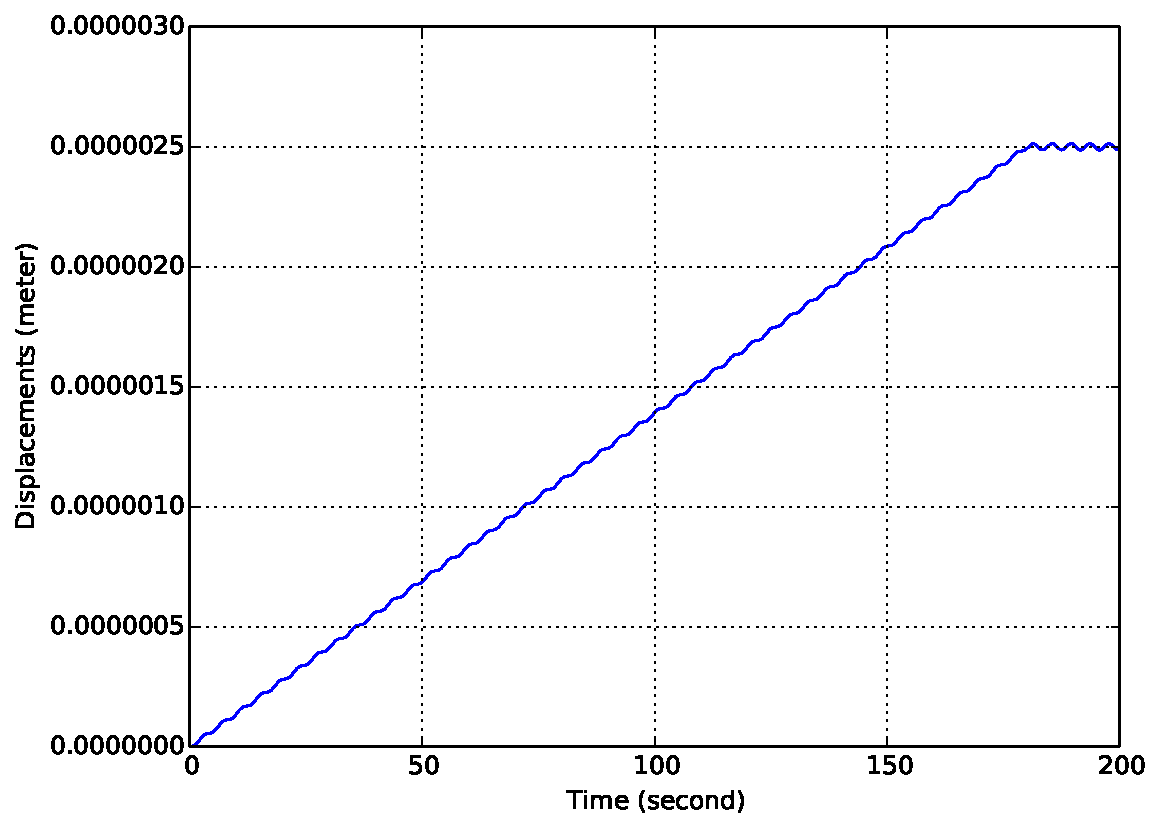
\includegraphics[width=12cm]{./Figure-files/_Chapter_Appendix_Illustrative_Examples/beam-mass-1element-slowLoading.pdf}
  \caption{Simulate the cantilever by 1 elastic beam element under the slow loading}
  \label{fig_beam-mass-slow}
\end{figure}


\begin{figure}[!htb]
  \centering
  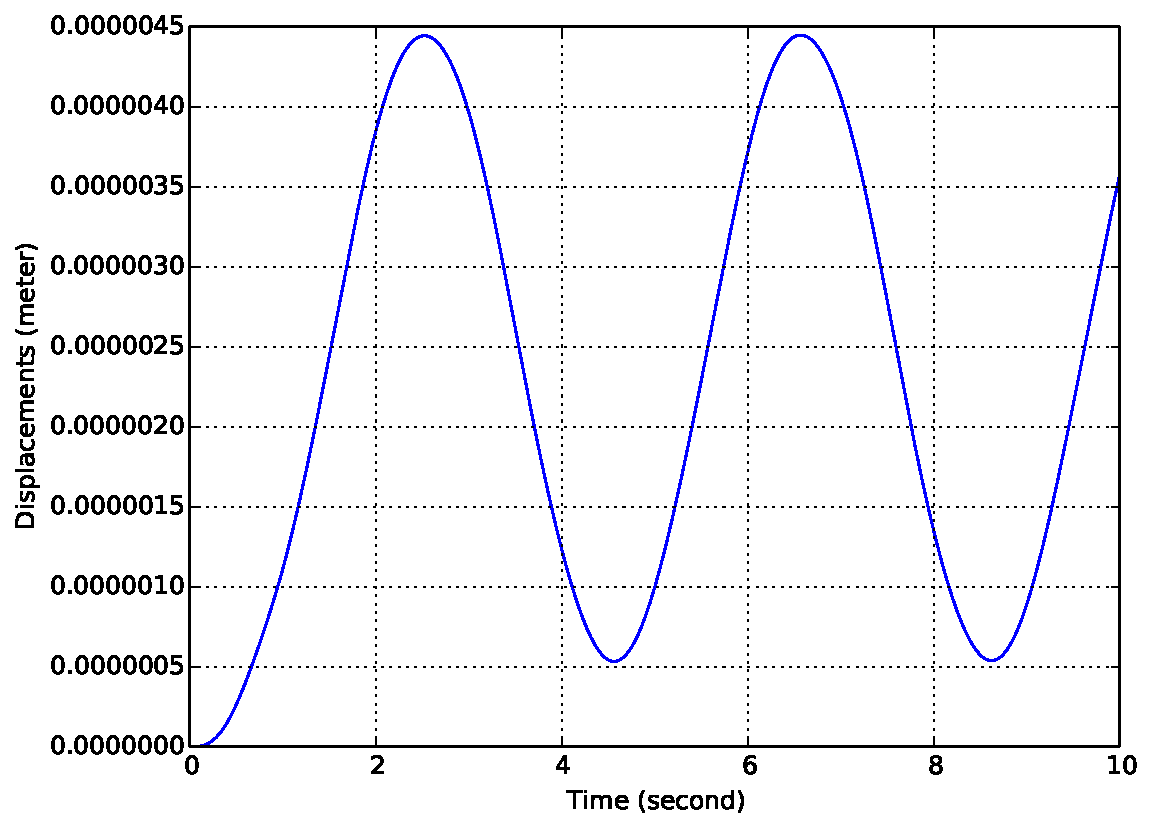
\includegraphics[width=12cm]{./Figure-files/_Chapter_Appendix_Illustrative_Examples/beam-mass-1element-fastLoading.pdf}
  \caption{Simulate the cantilever by 1 elastic beam element under the fast loading}
  \label{fig_beam-mass-fast}
\end{figure}

\begin{figure}[!htb]
  \centering
  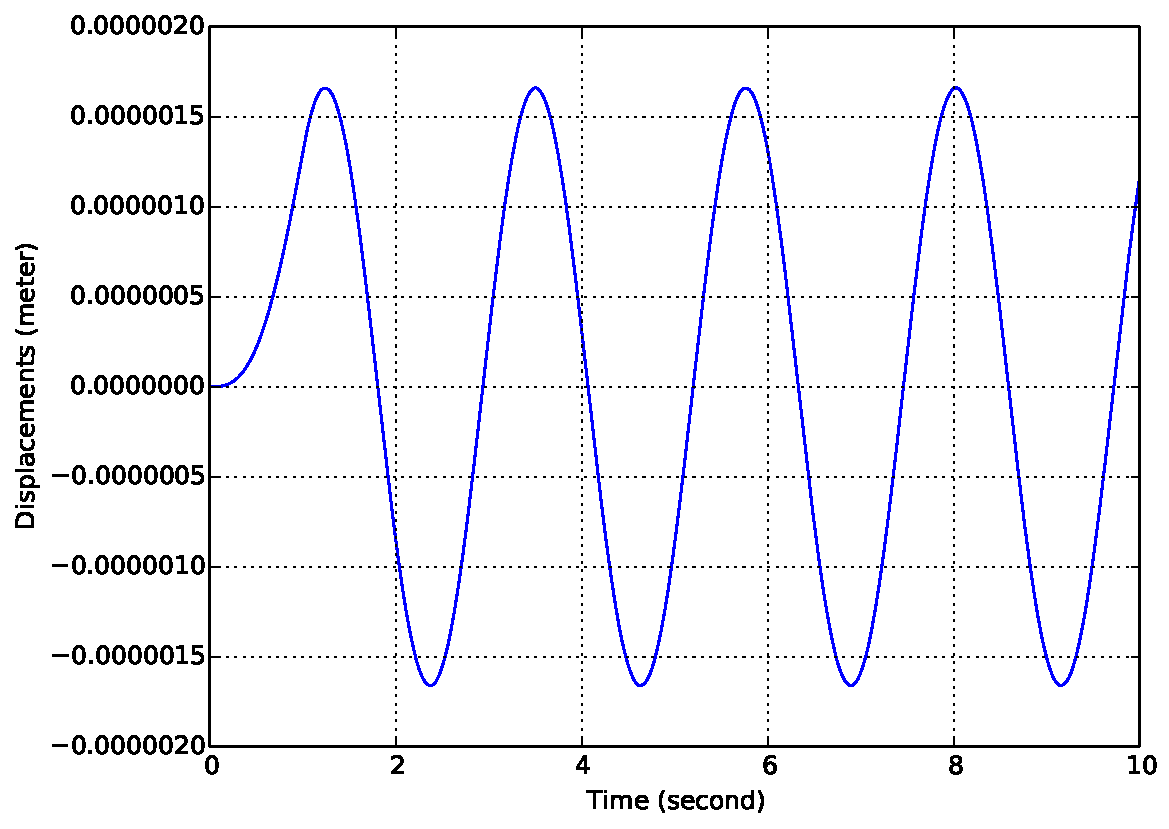
\includegraphics[width=12cm]{./Figure-files/_Chapter_Appendix_Illustrative_Examples/beam-mass-1element-freeVibration.pdf}
  \caption{Simulate the cantilever by 1 elastic beam element under the free vibration}
  \label{fig_beam-mass-freevibr}
\end{figure}













%%%%%%%%%%%%%%%%%%%%%%%%%%%%%%%%%%%%%%%%%%%%%%%%%%%%%%%%%%%%%%%%%%%%%%%%%%%%%%%%
%%%%%%%%%%%%%%%%%%%%%%%%%%%%%%%%%%%%%%%%%%%%%%%%%%%%%%%%%%%%%%%%%%%%%%%%%%%%%%%%
%%%%%%%%%%%%%%%%%%%%%%%%%%%%%%%%%%%%%%%%%%%%%%%%%%%%%%%%%%%%%%%%%%%%%%%%%%%%%%%%
%%%%%%%%%%%%%%%%%%%%%%%%%%%%%%%%%%%%%%%%%%%%%%%%%%%%%%%%%%%%%%%%%%%%%%%%%%%%%%%%
%%%%%%%%%%%%%%%%%%%%%%%%%%%%%%%%%%%%%%%%%%%%%%%%%%%%%%%%%%%%%%%%%%%%%%%%%%%%%%%%
%%%%%%%%%%%%%%%%%%%%%%%%%%%%%%%%%%%%%%%%%%%%%%%%%%%%%%%%%%%%%%%%%%%%
%%%%%%%%%%%%%%%%%%%%%%%%%%%%%%%%%%%%%%%%%%%%%%%%%%%%%%%%%%%%%%%%%%%%

\newpage
\section{27NodeBrick under Dynamic Loading with concentrated mass} ~ 
\subsection{Simulate the cantilever by one 27NodeBrick element} 
\paragraph{Problem description:} ~

\begin{itemize}
  \item Structure size

    Structure Length=1m, width=0.2m, height=0.2m.

  \item Element size

    Element length=1m, width=0.2m, height=0.2m.
\end{itemize}

\begin{figure}[!htb]
  \centering
  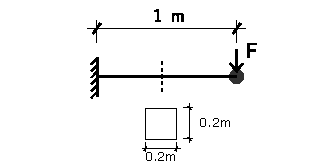
\includegraphics[width=12cm]{./Figure-files/_Chapter_Appendix_Illustrative_Examples/cantilever-mass.pdf}
  \caption{The cantilever-mass model}
  % \label{}
\end{figure}


\paragraph{ESSI model fei file: } ~

\begin{lstlisting}
model name "brick-mass_1element" ;

// Geometry: width and height
b=0.2*m;
h=0.2*m;

// Materials: properties
natural_period    = 1*s;        
natural_frequency  = 2*pi/natural_period;
elastic_constant  = 1e9*N/m^2; 
I=b*h^3/12.0;
A=b*h;
L=1*m;
rho   = (1.8751)^4*elastic_constant*I/(natural_frequency^2*L^4*A);
possion_ratio=0.3;

add material # 1 type linear_elastic_isotropic_3d_LT
  mass_density = rho
  elastic_modulus = elastic_constant
  poisson_ratio = possion_ratio;

add node #        1 at (   0.0000 *m,   0.2000 *m,  0.0000 *m) with 3 dofs;
add node #        2 at (   0.0000 *m,   0.0000 *m,  0.0000 *m) with 3 dofs;
add node #        3 at (   1.0000 *m,   0.2000 *m,  0.0000 *m) with 3 dofs;
add node #        4 at (   1.0000 *m,   0.0000 *m,  0.0000 *m) with 3 dofs;
add node #        5 at (   0.0000 *m,   0.0000 *m,  0.2000 *m) with 3 dofs;
add node #        6 at (   1.0000 *m,   0.0000 *m,  0.2000 *m) with 3 dofs;
add node #        7 at (   1.0000 *m,   0.2000 *m,  0.2000 *m) with 3 dofs;
add node #        8 at (   0.0000 *m,   0.2000 *m,  0.2000 *m) with 3 dofs;
add node #        9 at (   0.0000 *m,   0.1000 *m,  0.0000 *m) with 3 dofs;
add node #       10 at (   0.5000 *m,   0.2000 *m,  0.0000 *m) with 3 dofs;
add node #       11 at (   1.0000 *m,   0.1000 *m,  0.0000 *m) with 3 dofs;
add node #       12 at (   0.5000 *m,   0.0000 *m,  0.0000 *m) with 3 dofs;
add node #       13 at (   0.0000 *m,   0.1000 *m,  0.2000 *m) with 3 dofs;
add node #       14 at (   0.5000 *m,   0.2000 *m,  0.2000 *m) with 3 dofs;
add node #       15 at (   1.0000 *m,   0.1000 *m,  0.2000 *m) with 3 dofs;
add node #       16 at (   0.5000 *m,   0.0000 *m,  0.2000 *m) with 3 dofs;
add node #       17 at (   0.0000 *m,   0.0000 *m,  0.1000 *m) with 3 dofs;
add node #       18 at (   0.0000 *m,   0.2000 *m,  0.1000 *m) with 3 dofs;
add node #       19 at (   1.0000 *m,   0.2000 *m,  0.1000 *m) with 3 dofs;
add node #       20 at (   1.0000 *m,   0.0000 *m,  0.1000 *m) with 3 dofs;
add node #       21 at (   0.5000 *m,   0.1000 *m,  0.1000 *m) with 3 dofs;
add node #       22 at (   0.0000 *m,   0.1000 *m,  0.1000 *m) with 3 dofs;
add node #       23 at (   0.5000 *m,   0.2000 *m,  0.1000 *m) with 3 dofs;
add node #       24 at (   1.0000 *m,   0.1000 *m,  0.1000 *m) with 3 dofs;
add node #       25 at (   0.5000 *m,   0.0000 *m,  0.1000 *m) with 3 dofs;
add node #       26 at (   0.5000 *m,   0.1000 *m,  0.0000 *m) with 3 dofs;
add node #       27 at (   0.5000 *m,   0.1000 *m,  0.2000 *m) with 3 dofs;

add element #         1 type 27NodeBrickLT with nodes(       2,       1,       3,       4,       5,       8,       7,       6,       9,      10,      11,      12,      13,      14,      15,      16,      17,      18,      19,      20,      21,      22,      23,      24,      25,      26,      27) use material #        1; 

fix node # 1 dofs all;
fix node # 2 dofs all;
fix node # 5 dofs all;
fix node # 8 dofs all;
fix node # 9 dofs all;
fix node # 13 dofs all;
fix node # 17 dofs all;
fix node # 18 dofs all;
fix node # 22 dofs all;


// Mapping from 3 dofs to 6 dofs. 
add node #      1003 at (   1.0000 *m,   0.2000 *m,  0.0000 *m) with 6 dofs;
add node #      1004 at (   1.0000 *m,   0.0000 *m,  0.0000 *m) with 6 dofs;
add node #      1006 at (   1.0000 *m,   0.0000 *m,  0.2000 *m) with 6 dofs;
add node #      1007 at (   1.0000 *m,   0.2000 *m,  0.2000 *m) with 6 dofs;
// And connect the nodes at the same location.
add constraint equal dof with master node # 3 and slave node #  1003 dof to constrain ux uy uz;
add constraint equal dof with master node # 4 and slave node #  1004 dof to constrain ux uy uz;
add constraint equal dof with master node # 6 and slave node #  1006 dof to constrain ux uy uz;
add constraint equal dof with master node # 7 and slave node #  1007 dof to constrain ux uy uz;

add mass to node # 24   mx =  rho*A*L my =  rho*A*L mz = rho*A*L;

// add 6 beams to connect the mass 
smallb=0.01*m;
smallh=0.01*m;
smallE  = 1e9*N/m^2; 
smallnu=0.3;
smallrho=0*kg/m^3;
smallI=smallb*smallh^3/12.0;
add element # 11 type beam_elastic with nodes (1003,1004) 
  cross_section =   smallb*smallh 
  elastic_modulus =  smallE
  shear_modulus =  smallE/2/(1+smallnu)
  torsion_Jx =  0.33*smallb*smallh^3
  bending_Iy =  smallI
  bending_Iz =  smallI
  mass_density = smallrho
  xz_plane_vector = ( 1, 0, 1) 
  joint_1_offset = (0*m, 0*m, 0*m) 
  joint_2_offset = (0*m, 0*m, 0*m);
add element # 12 type beam_elastic with nodes (1003,1006) 
  cross_section =   smallb*smallh 
  elastic_modulus =  smallE
  shear_modulus =  smallE/2/(1+smallnu)
  torsion_Jx =  0.33*smallb*smallh^3
  bending_Iy =  smallI
  bending_Iz =  smallI
  mass_density = smallrho
  xz_plane_vector = ( 1, 0, 1) 
  joint_1_offset = (0*m, 0*m, 0*m) 
  joint_2_offset = (0*m, 0*m, 0*m);
add element # 13 type beam_elastic with nodes (1003,1007) 
  cross_section =   smallb*smallh 
  elastic_modulus =  smallE
  shear_modulus =  smallE/2/(1+smallnu)
  torsion_Jx =  0.33*smallb*smallh^3
  bending_Iy =  smallI
  bending_Iz =  smallI
  mass_density = smallrho
  xz_plane_vector = ( 1, 0, 1) 
  joint_1_offset = (0*m, 0*m, 0*m) 
  joint_2_offset = (0*m, 0*m, 0*m);
add element # 14 type beam_elastic with nodes (1004,1006) 
  cross_section =   smallb*smallh 
  elastic_modulus =  smallE
  shear_modulus =  smallE/2/(1+smallnu)
  torsion_Jx =  0.33*smallb*smallh^3
  bending_Iy =  smallI
  bending_Iz =  smallI
  mass_density = smallrho
  xz_plane_vector = ( 1, 0, 1) 
  joint_1_offset = (0*m, 0*m, 0*m) 
  joint_2_offset = (0*m, 0*m, 0*m);
add element # 15 type beam_elastic with nodes (1004,1007) 
  cross_section =   smallb*smallh 
  elastic_modulus =  smallE
  shear_modulus =  smallE/2/(1+smallnu)
  torsion_Jx =  0.33*smallb*smallh^3
  bending_Iy =  smallI
  bending_Iz =  smallI
  mass_density = smallrho
  xz_plane_vector = ( 1, 0, 1) 
  joint_1_offset = (0*m, 0*m, 0*m) 
  joint_2_offset = (0*m, 0*m, 0*m);
add element # 16 type beam_elastic with nodes (1006,1007) 
  cross_section =   smallb*smallh 
  elastic_modulus =  smallE
  shear_modulus =  smallE/2/(1+smallnu)
  torsion_Jx =  0.33*smallb*smallh^3
  bending_Iy =  smallI
  bending_Iz =  smallI
  mass_density = smallrho
  xz_plane_vector = ( 1, 0, 1) 
  joint_1_offset = (0*m, 0*m, 0*m) 
  joint_2_offset = (0*m, 0*m, 0*m);


// // ----------------------------------------------------------------------------
// // --slowLoading---------------------------------------------------------------
// // add the 1 Newton load in 180 seconds.
// // ----------------------------------------------------------------------------
// new loading stage "slowLoading";
// add load # 1 to node # 4 type path_time_series Fz=1/36.0*N series_file = "slowLoading.txt" ; 
// add load # 2 to node # 6 type path_time_series Fz=1/36.0*N series_file = "slowLoading.txt" ; 
// add load # 3 to node # 3 type path_time_series Fz=1/36.0*N series_file = "slowLoading.txt" ; 
// add load # 4 to node # 7 type path_time_series Fz=1/36.0*N series_file = "slowLoading.txt" ; 
// add load # 5 to node # 20 type path_time_series Fz=1/9.0*N series_file = "slowLoading.txt" ; 
// add load # 6 to node # 11 type path_time_series Fz=1/9.0*N series_file = "slowLoading.txt" ; 
// add load # 7 to node # 15 type path_time_series Fz=1/9.0*N series_file = "slowLoading.txt" ; 
// add load # 8 to node # 19 type path_time_series Fz=1/9.0*N series_file = "slowLoading.txt" ; 
// add load # 9 to node # 24 type path_time_series Fz=4/9.0*N series_file = "slowLoading.txt" ; 
// // add algorithm and solver
// define dynamic integrator Newmark with gamma = 0.5 beta = 0.25;
// define algorithm With_no_convergence_check ;
// define solver ProfileSPD;
// simulate 2000 steps using transient algorithm 
//  time_step = 0.1*s;

// // ----------------------------------------------------------------------------
// // --fastLoading---------------------------------------------------------------
// // add the 1 Newton load in 0.6 seconds.
// // ----------------------------------------------------------------------------
// new loading stage "fastLoading";
// add load # 101 to node # 4 type path_time_series Fz=1/36.0*N series_file = "fastLoading.txt" ; 
// add load # 102 to node # 6 type path_time_series Fz=1/36.0*N series_file = "fastLoading.txt" ; 
// add load # 103 to node # 3 type path_time_series Fz=1/36.0*N series_file = "fastLoading.txt" ; 
// add load # 104 to node # 7 type path_time_series Fz=1/36.0*N series_file = "fastLoading.txt" ; 
// add load # 105 to node # 20 type path_time_series Fz=1/9.0*N series_file = "fastLoading.txt" ; 
// add load # 106 to node # 11 type path_time_series Fz=1/9.0*N series_file = "fastLoading.txt" ; 
// add load # 107 to node # 15 type path_time_series Fz=1/9.0*N series_file = "fastLoading.txt" ; 
// add load # 108 to node # 19 type path_time_series Fz=1/9.0*N series_file = "fastLoading.txt" ; 
// add load # 109 to node # 24 type path_time_series Fz=4/9.0*N series_file = "fastLoading.txt" ; 
// // add algorithm and solver
// define dynamic integrator Newmark with gamma = 0.5 beta = 0.25;
// define algorithm With_no_convergence_check ;
// define solver ProfileSPD;
// simulate 1000 steps using transient algorithm 
//  time_step = 0.01*s;

// // ----------------------------------------------------------------------------
// // --freeVibration---------------------------------------------------------------
// // ----------------------------------------------------------------------------
new loading stage "freeVibration";
add load # 201 to node # 4 type path_time_series Fz=1/36.0*N series_file = "freeVibration.txt" ; 
add load # 202 to node # 6 type path_time_series Fz=1/36.0*N series_file = "freeVibration.txt" ; 
add load # 203 to node # 3 type path_time_series Fz=1/36.0*N series_file = "freeVibration.txt" ; 
add load # 204 to node # 7 type path_time_series Fz=1/36.0*N series_file = "freeVibration.txt" ; 
add load # 205 to node # 20 type path_time_series Fz=1/9.0*N series_file = "freeVibration.txt" ; 
add load # 206 to node # 11 type path_time_series Fz=1/9.0*N series_file = "freeVibration.txt" ; 
add load # 207 to node # 15 type path_time_series Fz=1/9.0*N series_file = "freeVibration.txt" ; 
add load # 208 to node # 19 type path_time_series Fz=1/9.0*N series_file = "freeVibration.txt" ; 
add load # 209 to node # 24 type path_time_series Fz=4/9.0*N series_file = "freeVibration.txt" ; 
// add algorithm and solver
define dynamic integrator Newmark with gamma = 0.5 beta = 0.25;
define algorithm With_no_convergence_check ;
define solver ProfileSPD;
simulate 100 steps using transient algorithm 
  time_step = 0.1*s;

// end
bye;
\end{lstlisting}

\paragraph{Displacement results against time series} ~

\begin{figure}[!htb]
  \centering
  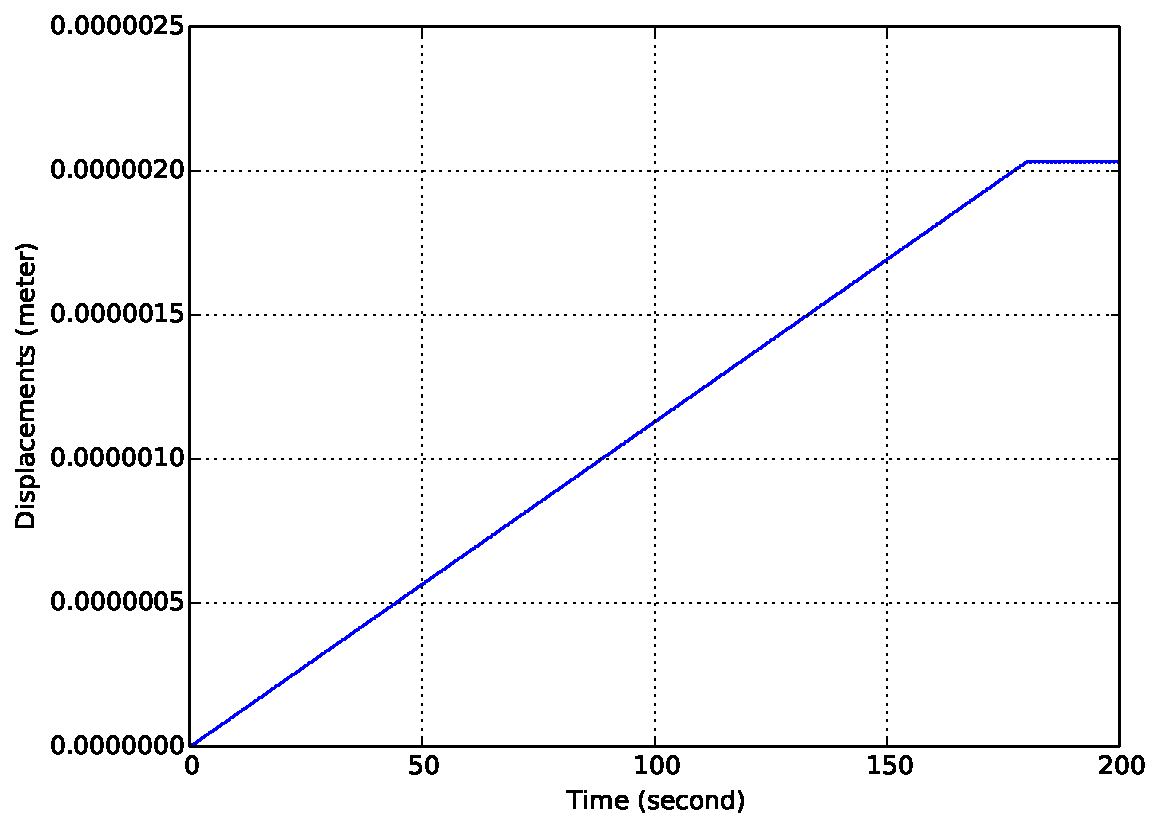
\includegraphics[width=12cm]{./Figure-files/_Chapter_Appendix_Illustrative_Examples/brick-mass-1element-slowLoading.pdf}
  \caption{Simulate the cantilever by one 27NodeBrick element under the slow loading}
  \label{fig_27brick-mass-slow}
\end{figure}


\begin{figure}[!htb]
  \centering
  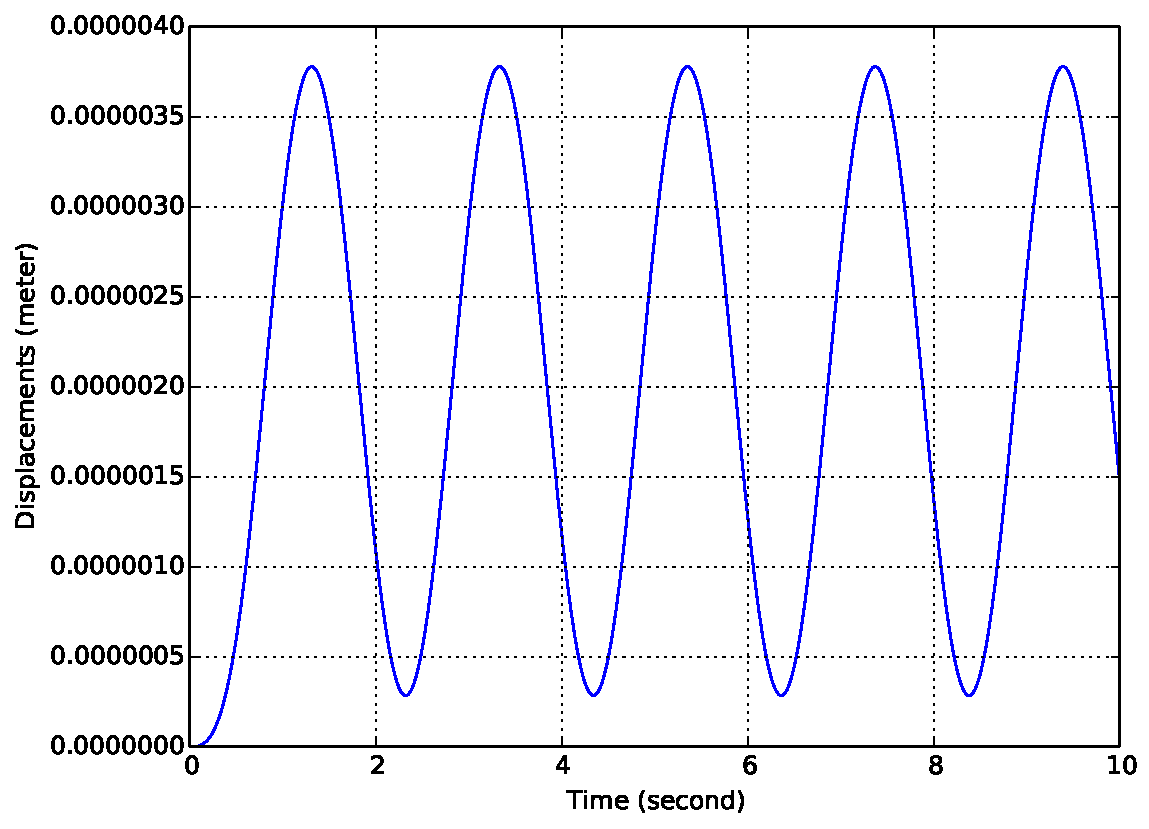
\includegraphics[width=12cm]{./Figure-files/_Chapter_Appendix_Illustrative_Examples/brick-mass-1element-fastLoading.pdf}
  \caption{Simulate the cantilever by one 27NodeBrick beam element under the fast loading}
  \label{fig_27brick-mass-fast}
\end{figure}

\begin{figure}[!htb]
  \centering
  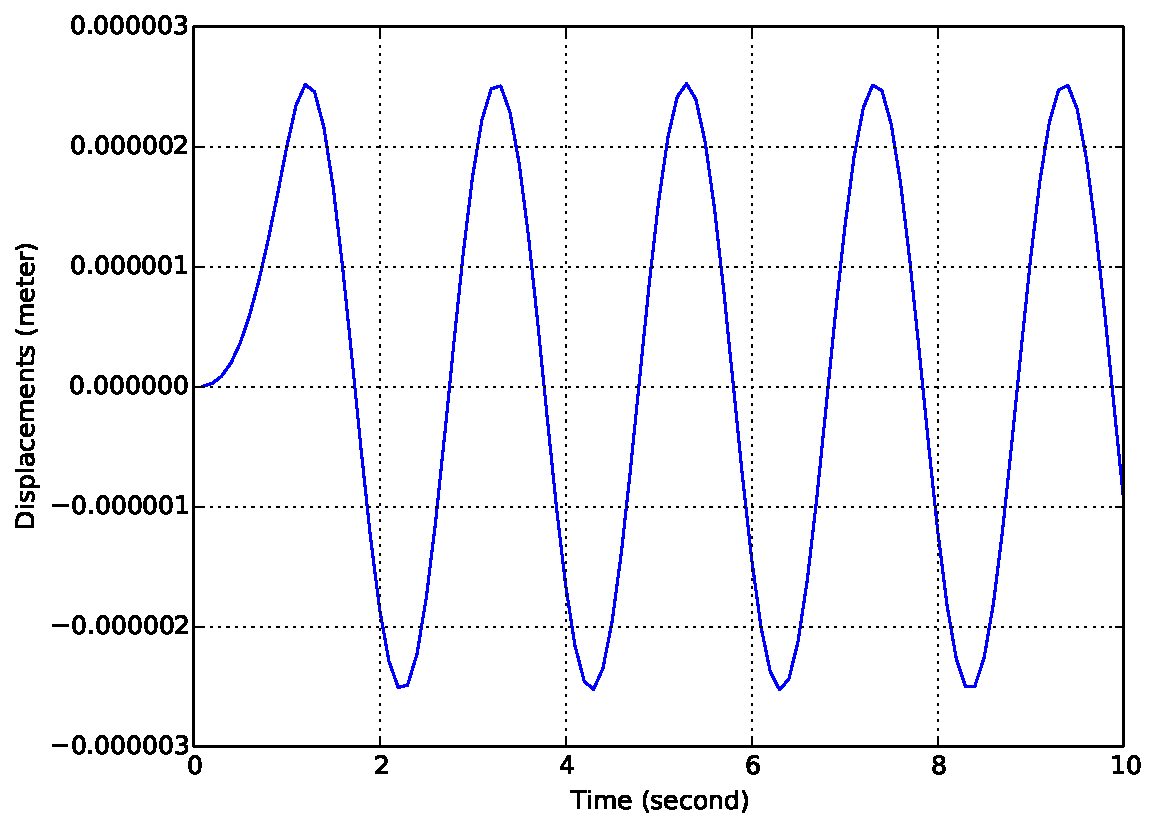
\includegraphics[width=12cm]{./Figure-files/_Chapter_Appendix_Illustrative_Examples/brick-mass-1element-freeVibration.pdf}
  \caption{Simulate the cantilever by one 27NodeBrick beam element under the free vibration}
  \label{fig_27brick-mass-freeVib}
\end{figure}

























%%%%%%%%%%%%%%%%%%%%%%%%%%%%%%%%%%%%%%%%%%%%%%%%%%%%%%%%%%%%%%%%%%%%%%%%%%%%%%%%
%%%%%%%%%%%%%%%%%%%%%%%%%%%%%%%%%%%%%%%%%%%%%%%%%%%%%%%%%%%%%%%%%%%%%%%%%%%%%%%%
%%%%%%%%%%%%%%%%%%%%%%%%%%%%%%%%%%%%%%%%%%%%%%%%%%%%%%%%%%%%%%%%%%%%%%%%%%%%%%%%
%%%%%%%%%%%%%%%%%%%%%%%%%%%%%%%%%%%%%%%%%%%%%%%%%%%%%%%%%%%%%%%%%%%%%%%%%%%%%%%%
%%%%%%%%%%%%%%%%%%%%%%%%%%%%%%%%%%%%%%%%%%%%%%%%%%%%%%%%%%%%%%%%%%%%%%%%%%%%%%%%
%%%%%%%%%%%%%%%%%%%%%%%%%%%%%%%%%%%%%%%%%%%%%%%%%%%%%%%%%%%%%%%%%%%%
%%%%%%%%%%%%%%%%%%%%%%%%%%%%%%%%%%%%%%%%%%%%%%%%%%%%%%%%%%%%%%%%%%%%

\newpage
\section{Elastic Beam Element under Dynamic Loading in different damping} ~ 
\subsection{Simulate the cantilever by 1 elastic beam element} 
\paragraph{Problem description:} ~

\begin{itemize}
  \item Structure size

    Structure Length=1m, width=0.2m, height=0.2m.

  \item Element size

    Element length=1m, width=0.2m, height=0.2m.
\end{itemize}

\begin{figure}[!htb]
  \centering
  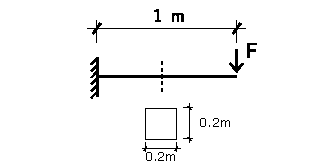
\includegraphics[width=12cm]{./Figure-files/_Chapter_Appendix_Illustrative_Examples/cantilever.pdf}
  \caption{The cantilever-mass model}
  \label{fig_cantilev_1beam_damping}
\end{figure}


\paragraph{ESSI model fei file: } ~

\begin{lstlisting}
model name "beam_1element" ;

// add node
add node #  1 at (   0.0*m ,    0.0*m,     0.0*m)  with 6 dofs;
add node #  2 at (   1.0*m ,    0.0*m,     0.0*m)  with 6 dofs;
  
// Geometry: width and height
b=0.2*m;
h=0.2*m;

// Materials: properties
natural_period    = 1*s;        
natural_frequency  = 2*pi/natural_period;
elastic_constant  = 1e9*N/m^2; 
I=b*h^3/12.0;
A=b*h;
L=1*m;
rho   = (1.8751)^4*elastic_constant*I/(natural_frequency^2*L^4*A);
possion_ratio=0.3;

// add elements
add element # 1 type beam_elastic with nodes (1,2) 
  cross_section =   b*h 
  elastic_modulus =  elastic_constant
  shear_modulus =  elastic_constant/2/(1+possion_ratio)
  torsion_Jx =  0.33*b*h^3
  bending_Iy =  b*h^3/12
  bending_Iz =  b*h^3/12
  mass_density = rho
  xz_plane_vector = ( 1, 0, 1) 
  joint_1_offset = (0*m, 0*m, 0*m) 
  joint_2_offset = (0*m, 0*m, 0*m);

// add boundary condition
fix node #      1 dofs all;

// // ----------------------------------------------------------------------------
// // --no-damping-------------------------------------------------------------
// // ----------------------------------------------------------------------------
// new loading stage "no-damping";
// add load # 1 to node # 2 type path_time_series 
//  Fz =  1.*N
//  series_file = "freeVibration.txt" ;
// define dynamic integrator Newmark with gamma = 0.5 beta = 0.25;
// define algorithm With_no_convergence_check ;
// define solver ProfileSPD;
// simulate 100 steps using transient algorithm 
//  time_step = 0.1*s;

// // ----------------------------------------------------------------------------
// // --Newmark-damping-------------------------------------------------------------
// // ----------------------------------------------------------------------------
// remove load # 2;
// new loading stage "Newmark-damping";
// add load # 3 to node # 2 type path_time_series 
//  Fz =  1.*N
//  series_file = "freeVibration.txt" ;
// define dynamic integrator Newmark with gamma = 0.6 beta = 0.3025;
// define algorithm With_no_convergence_check ;
// define solver ProfileSPD;
// simulate 100 steps using transient algorithm 
//  time_step = 0.1*s;

// // ----------------------------------------------------------------------------
// // --Rayleigh-damping-------------------------------------------------------------
// // ----------------------------------------------------------------------------
// remove load # 4;
// simulate using eigen algorithm number_of_modes = 2;
f1=0.996807/s;
f2=0.996807/s;
w1 = 2*pi*f1;
w2 = 2*pi*f2;
xi=0.05;
rayl_a1 = 2*xi/(w1 + w2);
rayl_a0 = rayl_a1*w1*w2;

add damping # 1 type Rayleigh with 
  a0 =  rayl_a0
  a1 =  rayl_a1
  stiffness_to_use = Initial_Stiffness;
add damping # 1 to element # 1;

new loading stage "Rayleigh-damping";
add load # 5 to node # 2 type path_time_series 
  Fz =  1.*N
  series_file = "freeVibration.txt" ;
define dynamic integrator Newmark with gamma = 0.5 beta = 0.25;
define algorithm With_no_convergence_check ;
define solver ProfileSPD;
simulate 100 steps using transient algorithm 
  time_step = 0.1*s;


bye;
\end{lstlisting}

\paragraph{Displacement results against time series} ~

\begin{figure}[!htb]
  \centering
  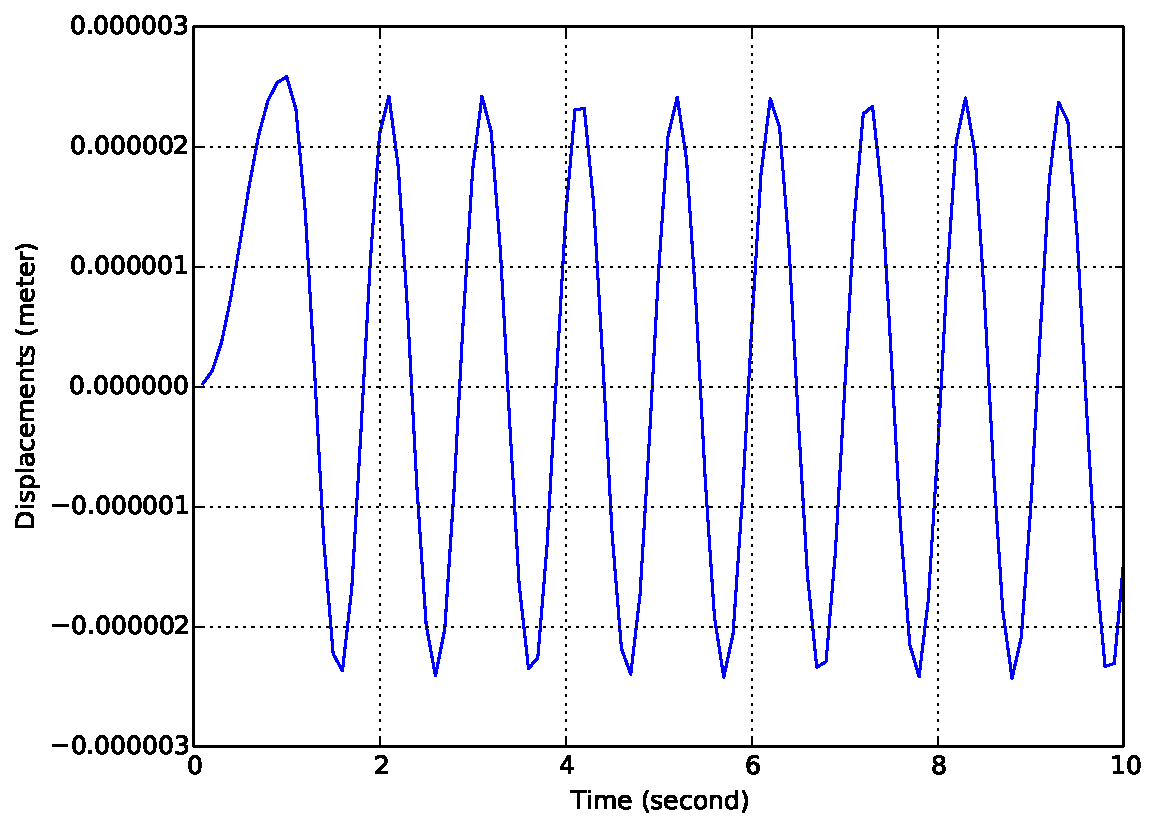
\includegraphics[width=12cm]{./Figure-files/_Chapter_Appendix_Illustrative_Examples/beam-1element-no-damping.pdf}
  \caption{Simulate the cantilever by 1 elastic beam element without damping}
  \label{fig_1beam_nodamping}
\end{figure}


\begin{figure}[!htb]
  \centering
  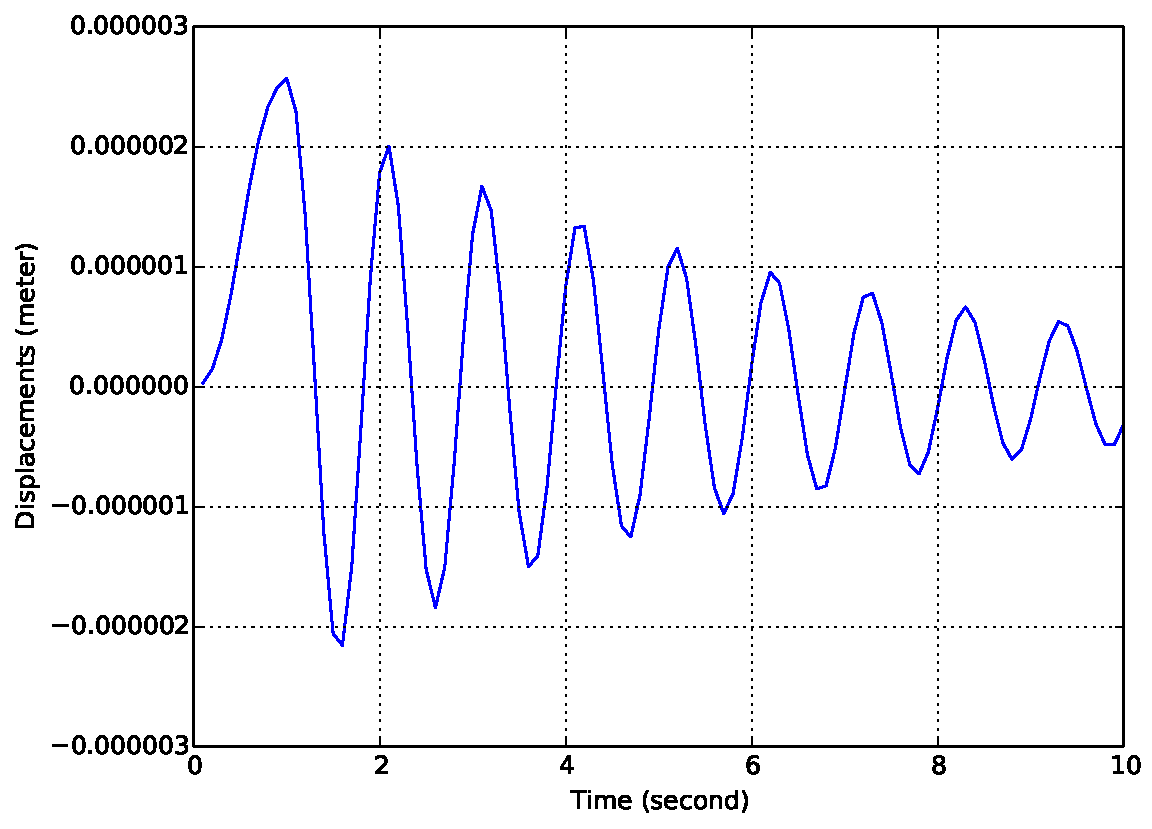
\includegraphics[width=12cm]{./Figure-files/_Chapter_Appendix_Illustrative_Examples/beam-1element-Newmark-damping.pdf}
  \caption{Simulate the cantilever by 1 elastic beam element with Newmark damping}
  \label{fig_1beam_newmark}
\end{figure}

\begin{figure}[!htb]
  \centering
  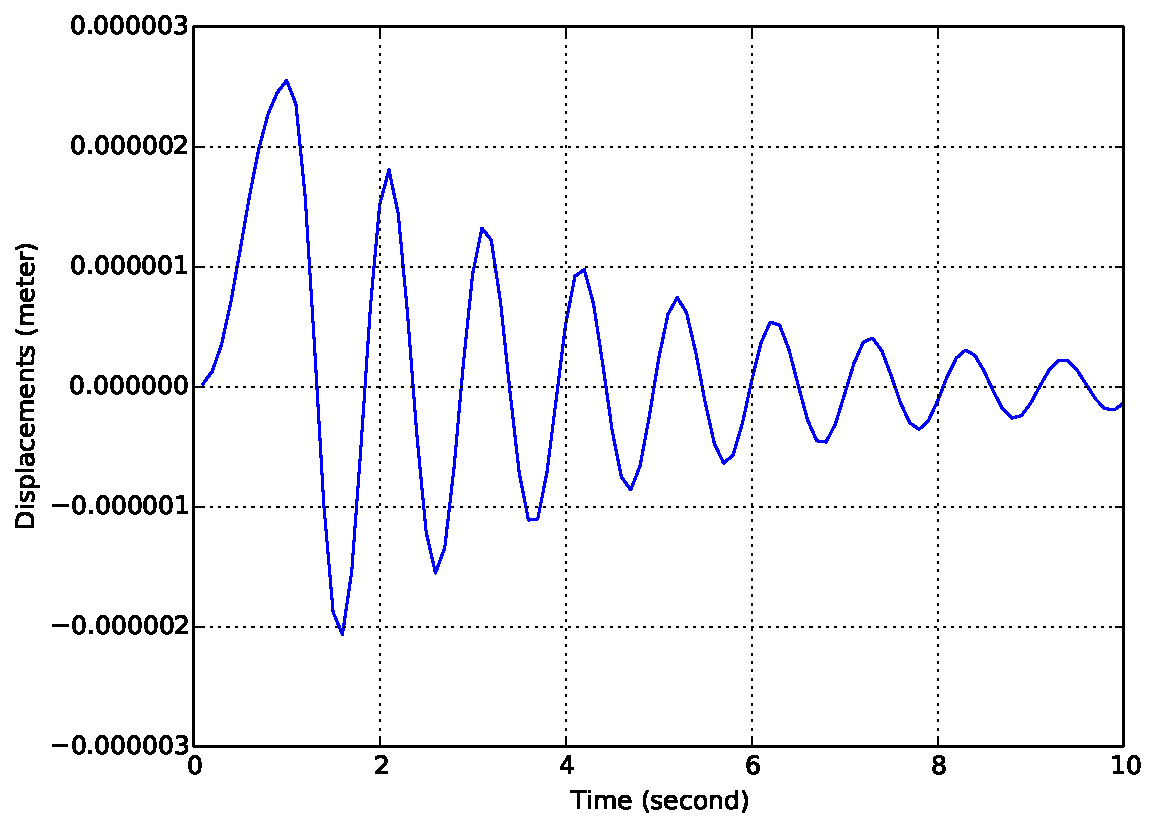
\includegraphics[width=12cm]{./Figure-files/_Chapter_Appendix_Illustrative_Examples/beam-1element-Rayleigh-damping.pdf}
  \caption{Simulate the cantilever by 1 elastic beam element with Rayleigh damping}
  \label{fig_1beam_rayleigh}
\end{figure}




